% main.tex: root file of the thesis.
% Build: latexmk -pdf -interaction=nonstopmode main.tex
\documentclass[12pt,a4paper,oneside]{report}
% preamble.tex: packages, page layout and project macros. Loaded by main.tex.

% ---------------------------------------------------------------------------
% Encoding, language and fonts
% ---------------------------------------------------------------------------
\usepackage[T1]{fontenc}
\usepackage{lmodern}
\usepackage[british]{babel}
% Heading of the table of contents (set through babel, which would otherwise
% reset it to "Contents").
\addto\captionsbritish{\renewcommand{\contentsname}{Table of Contents}}
\usepackage{csquotes}   % required by biblatex-apa
\usepackage{microtype}

% ---------------------------------------------------------------------------
% Page layout
% TODO: check margins, line spacing and font against the University of Benin
% School of Postgraduate Studies (SPGS) formatting rules. These are defaults
% chosen on 2026-11-02: A4, 12 pt (set in main.tex), 1.5 line spacing, wider
% left margin for binding.
% ---------------------------------------------------------------------------
\usepackage[a4paper,top=25mm,bottom=25mm,left=35mm,right=25mm]{geometry}
\usepackage{setspace}
\onehalfspacing

% ---------------------------------------------------------------------------
% Mathematics, units, tables, figures and lists
% ---------------------------------------------------------------------------
\usepackage{amsmath}
\usepackage{siunitx}
\sisetup{range-phrase={--}, range-units=single}
\usepackage{booktabs}
\usepackage{array}
\usepackage{tabularx}
\usepackage{graphicx}
\graphicspath{{figures/}}
% Figure and table captions in italics, so they stand apart from the body text
% (author's request, 2 November 2026).
\usepackage{caption}
\captionsetup{font=it}
\usepackage{enumitem}
\usepackage{xcolor}
\usepackage[nottoc,notbib]{tocbibind}   % lists of tables and figures in the TOC
% Code listings (Appendix B, author's request 2 November 2026). Box-drawing and
% other non-ASCII characters in the code are mapped to printable equivalents.
\usepackage{listings}
\lstset{
  language=Python,
  basicstyle=\ttfamily\scriptsize,
  numbers=left, numberstyle=\tiny\color{gray}, numbersep=5pt, xleftmargin=1.6em,
  frame=lines, framesep=2pt,
  breaklines=true, postbreak=\mbox{\textcolor{gray}{$\hookrightarrow$}\space},
  showstringspaces=false, keepspaces=true, columns=fixed, basewidth=0.525em, tabsize=4, upquote=true,
  keywordstyle=\color{blue!55!black}, commentstyle=\color{green!35!black},
  stringstyle=\color{red!50!black},
  extendedchars=true,
  literate={─}{{-}}1 {—}{{---}}1 {–}{{--}}1 {→}{{$\rightarrow$}}1 {←}{{$\leftarrow$}}1
           {×}{{$\times$}}1 {≤}{{$\le$}}1 {≥}{{$\ge$}}1 {±}{{$\pm$}}1 {µ}{{$\mu$}}1
           {Ω}{{$\Omega$}}1 {°}{{$^\circ$}}1 {…}{{...}}3 {σ}{{$\sigma$}}1 {α}{{$\alpha$}}1
           {γ}{{$\gamma$}}1 {κ}{{$\kappa$}}1 {λ}{{$\lambda$}}1 {ρ}{{$\rho$}}1 {Δ}{{$\Delta$}}1
           {²}{{$^2$}}1 {√}{{$\surd$}}1 {≈}{{$\approx$}}1 {·}{{$\cdot$}}1
}

% ---------------------------------------------------------------------------
% Bibliography: APA 7 (biblatex-apa) with biber
% ---------------------------------------------------------------------------
\usepackage[style=apa,backend=biber]{biblatex}
\addbibresource{bib/references.bib}
% APA 7 puts a comma before "&" in lists of three or more names; British
% English settings would drop it.
\DefineBibliographyExtras{british}{\def\finalandcomma{\addcomma}}
% Allow line breaks inside long DOIs and URLs.
\setcounter{biburlnumpenalty}{100}
\setcounter{biburlucpenalty}{100}
\setcounter{biburllcpenalty}{100}
% Let the reference list break lines more loosely, so that long unbreakable
% items (URLs, arXiv identifiers) move to the next line instead of overflowing
% the margin.
\appto{\bibsetup}{\sloppy}

% ---------------------------------------------------------------------------
% Hyperlinks and cross-references (hyperref must load before cleveref)
% ---------------------------------------------------------------------------
\usepackage[hidelinks]{hyperref}
\usepackage[capitalise,noabbrev]{cleveref}

% ---------------------------------------------------------------------------
% Placeholders: printed in red until resolved, so none can be missed
% ---------------------------------------------------------------------------
\newcommand{\TBC}[1]{\textcolor{red}{[#1]}}
% Provisional value: a starting setting that may still be tuned on training and
% validation data (notes/method-design.md, "[default]"). Red until frozen.
\newcommand{\Prov}[1]{\textcolor{red}{#1}}
% The band studied, chosen after the band survey and confirmed by the author on
% 5 November 2026 (Appendix A).
\newcommand{\TargetBand}{LTE Band~28, downlink \qtyrange{758}{803}{\mega\hertz}}

% ---------------------------------------------------------------------------
% Thesis metadata (title page, declaration, certification, PDF properties)
% ---------------------------------------------------------------------------
% Final title, chosen by the author on 4 November 2026.
\newcommand{\ThesisTitle}{AI-Based LTE Spectrum Occupancy Detection Using Autoencoders and a Low-Cost RTL-SDR: A Session-Level Evaluation Against Classical Detectors}
\newcommand{\ThesisAuthor}{Jimrox Odezi Ogume}
\newcommand{\ThesisDepartment}{Department of Electrical and Electronic Engineering}
\newcommand{\ThesisUniversity}{University of Benin}
\newcommand{\ThesisPlace}{Benin City, Nigeria}
\newcommand{\ThesisDegree}{Master of Science (M.Sc.) in Electrical and Electronic Engineering}
\newcommand{\ThesisSupervisor}{Prof.\ Kingsley Ogbeide}
\newcommand{\ThesisHoD}{\TBC{Head of Department's name}}
\newcommand{\ThesisDate}{\TBC{month and year of submission}}

\hypersetup{
  pdftitle  = {AI-Based LTE Spectrum Occupancy Detection Using Autoencoders and a Low-Cost RTL-SDR: A Session-Level Evaluation Against Classical Detectors},
  pdfauthor = {Jimrox Odezi Ogume},
}

% ---------------------------------------------------------------------------
% Notation (keep in step with front/abbreviations.tex)
% ---------------------------------------------------------------------------
\newcommand{\Pd}{P_{\mathrm{D}}}    % probability of detection
\newcommand{\Pfa}{P_{\mathrm{FA}}}  % probability of false alarm
% Percentages without a space before the sign, as in APA style.
\newcommand{\pct}[1]{\qty[quantity-product={}]{#1}{\percent}}

% ---------------------------------------------------------------------------
% Terms
% ---------------------------------------------------------------------------
% Prints "synchronization-signal". An explicit hyphen would stop TeX from
% hyphenating "synchronization" and cause overfull lines; babel's hard hyphen
% keeps the hyphen and still allows normal hyphenation of the word.
\newcommand{\syncsignal}{synchronization\babelhyphen{hard}signal}


\begin{document}

% ---------------------------------------------------------------------------
% Preliminary pages (lower-case roman page numbers; the title page counts as i)
% TODO: check the order and wording of these pages against the SPGS rules.
% ---------------------------------------------------------------------------
\pagenumbering{roman}
% front/titlepage.tex: title page. Metadata macros are defined in preamble.tex.
% TODO: confirm the final title, the degree wording and whether the
% registration number must appear (SPGS rules).
\begin{titlepage}
  \centering
  {\Large\bfseries\MakeUppercase{\ThesisTitle}\par}
  \vspace{2.5cm}
  {\large BY\par}
  \vspace{0.8cm}
  {\large\bfseries\MakeUppercase{\ThesisAuthor}\par}
  \vspace{2.5cm}
  {A thesis submitted to the \ThesisDepartment,\\
   \ThesisUniversity, in partial fulfilment of the requirements\\
   for the award of the degree of\\[0.5em]
   \textbf{\ThesisDegree}\par}
  \vspace{0.5em}
  {\small\TBC{confirm the submission wording against the SPGS rules}\par}
  \vfill
  {\large\MakeUppercase{\ThesisDepartment}\\
   \MakeUppercase{\ThesisUniversity}\\
   \ThesisPlace\par}
  \vspace{1cm}
  {\large\ThesisDate\par}
\end{titlepage}

\setcounter{page}{2}   % titlepage resets the counter; the next page is ii
% front/declaration.tex: candidate's declaration.
% TODO: replace with the SPGS wording if one is prescribed.
\chapter*{Declaration}
\addcontentsline{toc}{chapter}{Declaration}

I declare that this thesis is my own work, carried out in the \ThesisDepartment,
\ThesisUniversity, under the supervision of \ThesisSupervisor. It has not been
submitted, in whole or in part, for any other degree, and all sources of
information have been acknowledged by means of references.

\vspace{3cm}
\noindent
\begin{tabular}{@{}p{0.45\textwidth}@{\hspace{0.1\textwidth}}p{0.3\textwidth}@{}}
  \rule{\linewidth}{0.4pt} & \rule{\linewidth}{0.4pt} \\
  \ThesisAuthor            & Date \\
\end{tabular}

% front/certification.tex: certification by the supervisor and the Head of
% Department. TODO: confirm the required signatories and wording (SPGS rules);
% an external examiner or the Dean may also be required.
\chapter*{Certification}
\addcontentsline{toc}{chapter}{Certification}

This is to certify that the work reported in this thesis was carried out by
\ThesisAuthor{} in the \ThesisDepartment, \ThesisUniversity, under my
supervision.

\vspace{2.5cm}
\noindent
\begin{tabular}{@{}p{0.45\textwidth}@{\hspace{0.1\textwidth}}p{0.3\textwidth}@{}}
  \rule{\linewidth}{0.4pt} & \rule{\linewidth}{0.4pt} \\
  \ThesisSupervisor        & Date \\
  Supervisor               & \\[2.5cm]
  \rule{\linewidth}{0.4pt} & \rule{\linewidth}{0.4pt} \\
  \ThesisHoD               & Date \\
  Head of Department       & \\
\end{tabular}

\vspace{1cm}
\noindent\TBC{confirm the required signatories against the SPGS rules}

% front/dedication.tex: to be written by the author (optional page).
\chapter*{Dedication}
\addcontentsline{toc}{chapter}{Dedication}

\TBC{Dedication to be written by the author.}

% front/acknowledgements.tex: to be written by the author.
\chapter*{Acknowledgements}
\addcontentsline{toc}{chapter}{Acknowledgements}

\TBC{Acknowledgements to be written by the author.}

% front/abstract.tex: written last, once the results in Chapter 4 are final.
% It must report actual results from code/ and results/, never the hypotheses.
\chapter*{Abstract}
\addcontentsline{toc}{chapter}{Abstract}

\TBC{The abstract will be written once the results in Chapter~4 are final.}

\tableofcontents
\listoftables
\listoffigures
% front/abbreviations.tex: list of abbreviations and symbols.
% Maintained by hand: add an entry whenever a chapter defines a new acronym or
% symbol, and keep the symbols in step with the notation macros in preamble.tex.
% Current contents: everything defined in Chapter 1.
\chapter*{List of Abbreviations and Symbols}
\addcontentsline{toc}{chapter}{List of Abbreviations and Symbols}

\section*{Abbreviations}
\begin{description}[style=sameline, leftmargin=3.6cm, labelwidth=3.3cm, font=\normalfont, itemsep=0pt]
  \item[2G]           Second-generation (mobile networks)
  \item[3G]           Third-generation (mobile networks)
  \item[4G]           Fourth-generation (mobile networks)
  \item[5G]           Fifth-generation (mobile networks)
  \item[ADC]          Analogue-to-digital converter
  \item[AUC]          Area under the receiver operating characteristic curve
  \item[CFAR]         Constant false-alarm rate
  \item[CNN]          Convolutional neural network
  \item[CPU]          Central processing unit
  \item[GPU]          Graphics processing unit
  \item[H]            Hypothesis (H1, H2)
  \item[IMT-Advanced] International Mobile Telecommunications-Advanced
  \item[IQ]           In-phase and quadrature
  \item[LSTM]         Long short-term memory
  \item[LTE]          Long Term Evolution
  \item[MSE]          Mean squared error
  \item[NCC]          Nigerian Communications Commission
  \item[OFDM]         Orthogonal frequency-division multiplexing
  \item[PCA]          Principal component analysis
  \item[ROC]          Receiver operating characteristic
  \item[RQ]           Research question (RQ1--RQ5)
  \item[SDR]          Software-defined radio
  \item[SNR]          Signal-to-noise ratio
  \item[STFT]         Short-time Fourier transform
  \item[USRP]         Universal Software Radio Peripheral
  \item[VAE]          Variational autoencoder
  \item[VHF]          Very high frequency
\end{description}

\section*{Symbols}
\begin{description}[style=sameline, leftmargin=3.6cm, labelwidth=3.3cm, font=\normalfont, itemsep=0pt]
  \item[$\Pd$]  Probability of detection
  \item[$\Pfa$] Probability of false alarm
\end{description}


% ---------------------------------------------------------------------------
% Main text (arabic page numbers from 1). The \clearpage must come before
% \pagenumbering, or the last preliminary page would be renumbered 1.
% ---------------------------------------------------------------------------
\clearpage
\pagenumbering{arabic}
% chapters/chapter1.tex: Chapter 1, Introduction.
% Outline approved 2 November 2026 (notes/chapter1-outline.md).
% Claims and their sources: notes/chapter1-claims.md.
% References to Chapters 2-5 are plain text until those chapters carry labels;
% switch them to \cref{ch:...} then.
% TODO: revisit the contributions (Section 1.6) once Chapter 4 results exist.
% TODO: re-check the gap statement (end of Section 1.2) after the Chapter 2
%       literature search.

\chapter{Introduction}
\label{ch:introduction}

This thesis evaluates whether an autoencoder trained only on idle spectrum, captured with a low-cost RTL-SDR receiver, can detect when a Long Term Evolution (LTE) downlink band is occupied, and compares it with classical detectors tuned with equal care. This chapter sets out the background and motivation (\cref{sec:background}), the problem (\cref{sec:problem}), the aim, research questions and hypotheses (\cref{sec:aim}), the objectives (\cref{sec:objectives}), the scope (\cref{sec:scope}) and the contributions (\cref{sec:contributions}) of the study, and outlines the remaining chapters (\cref{sec:organization}).

% ===========================================================================
\section{Background and Motivation}
\label{sec:background}

\subsection{Spectrum Use and Its Measurement}
\label{sec:spectrum-use}

The radio spectrum is the natural resource on which wireless communication depends. It has traditionally been regulated by assigning bands to licensed users on a long-term basis, with the aim of keeping wireless systems free of harmful interference \parencite{popoola2018}. Measurements of how assigned spectrum is actually used have shown that much of it is idle for much of the time, and that its use varies with time, frequency and location \parencite{axell2010,popoola2018}. In Nigeria, \textcite{popoola2018} measured occupancy over \qtyrange{80}{2200}{\mega\hertz} at sites in Abuja, Lafia, Lokoja, Gusau and Port Harcourt, and found an average occupancy below \pct{10} across that range. Occupancy measurements of this kind are the main quantitative tool through which regulators, researchers, engineers and policymakers learn how licensed bands are used in practice \parencite[p.~949]{popoola2018}.

The \textcite{itu2010} stated that International Mobile Telecommunications-Advanced (IMT-Advanced) systems are considered fourth-generation (4G) systems. It determined that LTE-Advanced should be designated an IMT-Advanced technology and noted that the term 4G may also be applied to LTE, its forerunner. In Nigeria, 4G is now the mobile generation used by the largest share of subscribers. In August 2026, \pct{54.77} of mobile subscribers used 4G services, against \pct{36.05} for second-generation (2G), \pct{4.27} for third-generation (3G) and \pct{4.92} for fifth-generation (5G) services \parencite{ncc2026}. The LTE downlink, which carries transmissions from base stations to users' devices, is therefore of direct practical interest. LTE is one of several current systems that use orthogonal frequency-division multiplexing (OFDM) signalling \parencite{axell2010}; the structure of the LTE downlink is reviewed in Chapter~2.

\subsection{Why Downlink Occupancy Matters}
\label{sec:why}

Knowing whether, when and where an LTE downlink band is occupied serves three purposes: interference management, network optimization and the planning of dynamic spectrum access.

\paragraph{Interference management.}
In each country, the radio spectrum is managed by authorities whose functions include monitoring radio emissions in order to identify, locate and eliminate harmful interference and other irregularities \parencite[p.~2]{torio2025}. Effective surveillance is needed to identify unauthorized emissions and mitigate interference. It has traditionally been carried out manually by surveillance teams, which is time-consuming, resource-intensive and prone to error when large parts of the spectrum must be watched in real time \parencite[p.~1]{torio2025}. Spectrum measurements are still made mainly by government agencies with bulky and expensive equipment, an approach that does not scale and gives only limited awareness of how the spectrum is actually used \parencite{calvopalomino2015}. Meanwhile, the risk of interference and malicious use of the spectrum has grown \parencite{tian2022}. An automated occupancy detector addresses the first step of this task: deciding, frame by frame, whether a band contains anything other than noise.

\paragraph{Network optimization.}
Interference also affects operators directly: illegal repeaters frequently disrupt mobile operators' cell planning, causing poor coverage and dropped connections \parencite{tian2022}. More generally, occupancy measurements give engineers and regulators information on how licensed bands are actually used \parencite[p.~949]{popoola2018}, and that use varies with time, frequency and location \parencite{popoola2018}. Low-cost sensors have been proposed as a way to make spectrum measurement continuous and large-scale \parencite{calvopalomino2015}. Their value for planning depends on whether their occupancy decisions can be trusted.

\paragraph{Dynamic spectrum access planning.}
Licensed spectrum is intended for use by its licence holders, and cognitive radio is a concept for reusing it in an unlicensed manner, motivated by measurements showing unused spectrum in frequency, time and space \parencite{axell2010}. Under such dynamic spectrum access, secondary users would use idle portions of licensed spectrum opportunistically, and before they can do so it must be established which portions are idle \parencite[p.~960]{popoola2018}. The licensed (primary) users must also be detected reliably enough that secondary users do not cause them harmful interference \parencite{tandra2008}. \Textcite{popoola2018} concluded that the low occupancy they measured suggests a hopeful future for dynamic spectrum access in Nigeria. Whatever band is considered, reliable occupancy detection is a prerequisite for such access. Cognitive radio is reviewed in Chapter~2.

\subsection{Low-Cost Software-Defined Radio as a Sensor}
\label{sec:low-cost-sdr}

In a software-defined radio (SDR), receiver functions that are traditionally implemented in hardware, such as mixing, filtering, demodulation and detection, are implemented in software instead \parencite{saber2021}. Receivers from the low-cost RTL-SDR family make this approach inexpensive. \Textcite{calvopalomino2015} built a wideband spectrum-monitoring sensor around an RTL-SDR-compatible USB dongle, which delivered digital in-phase and quadrature (IQ) samples to a host computer for processing. The sensor covered \qtyrange{24}{1766}{\mega\hertz} at a cost of under US\$100, which they put at 50 to 500 times cheaper than professional equipment.

The receiver used in this study, the RTL-SDR Blog V4, tunes from \qty{500}{\kilo\hertz} to \qty{1.766}{\giga\hertz}, digitizes the signal with an 8-bit analogue-to-digital converter (ADC) and has a stable bandwidth of about \qty{2.56}{\mega\hertz} \parencite{rtlsdrblog2024}. These figures bound the study. Only LTE downlink bands below about \qty{1.77}{\giga\hertz} can be received, and only a slice a few megahertz wide can be observed at once. The low cost also comes with limited amplitude resolution and dynamic range, which matter for detection at low signal-to-noise ratio (SNR), as \cref{sec:problem} explains.

\subsection{Learned Detection by Reconstruction Error}
\label{sec:learned-detection}

A detector need not model the signal it is looking for; it can model the noise instead. A model trained only on noise learns to reproduce noise-only observations, so an observation that it reconstructs poorly is evidence that something other than noise is present. An autoencoder suits this approach: it is a neural network that compresses its input into a smaller latent representation and reconstructs the input from that representation \parencite[pp.~2--3]{torio2025}. \Textcite{torio2025} applied this reasoning to spectrum surveillance. They trained an autoencoder on synthetic Rayleigh-distributed noise sequences, treated the absence of transmissions as the normal state of a channel, and took a large reconstruction error as evidence of a transmission (p.~5). Unsupervised models of this kind have also been used for spectrum anomaly detection more generally. \Textcite{tian2022}, for example, modelled spectrograms with a variational autoencoder (VAE) and scored anomalies with a percentile-based measure of the reconstruction error. In this thesis, the noise model is learned from idle spectrum captured with the RTL-SDR itself, so an LTE carrier is the anomaly to be detected. Autoencoders and the related literature are reviewed in Chapter~2.

% ===========================================================================
\section{Statement of the Problem}
\label{sec:problem}

Energy detection is a good choice for blind detection, that is, detection without knowledge of the signal \parencite{gao2019}. An energy detector compares the energy received during an observation interval with a threshold; it can detect any type of signal and needs no knowledge of the signal's structure \parencite{axell2010}. Its weakness lies in the threshold. Setting the threshold requires the noise variance, and if the noise variance is known only imperfectly, the threshold is wrong and performance deteriorates quickly \parencite{axell2010}. \Textcite{tandra2008} showed that, under such noise uncertainty, a detector with no knowledge of the signal's modulation cannot be made robust below a certain SNR, however long it observes the channel. They called this limit the \enquote{SNR wall}, and showed that any such detector is essentially as non-robust as the energy detector.

Noise uncertainty arises in every practical receiver. The noise that a receiver sees aggregates thermal noise, leakage of signals from other bands through receiver non-linearity, aliasing from imperfect front-end filters and interference from distant transmitters, so some uncertainty in the noise level remains even after calibration at run time \parencite{tandra2008}. Low-cost hardware adds a further limit. The RTL-SDR Blog V4 digitizes with an 8-bit ADC \parencite{rtlsdrblog2024}, which restricts its dynamic range. \Textcite{tandra2005} showed that, for a primary signal without a deterministic component, a receiver with a finite dynamic range faces an SNR wall that no detector can overcome, even under moderate noise uncertainty. Detectors that exploit known structure in the transmitted signal \parencite{axell2010} need prior knowledge of that signal, and \textcite{tandra2008} showed that coherent and cyclostationary feature detectors also lose robustness to model uncertainty when channel coherence times are finite.

Learned detectors have been proposed as a way past these limits, with mixed results. \Textcite{gao2019} reported a deep-learning detector whose SNR wall was \qty{3.15}{\decibel} lower than that of the energy detector at one operating point; their signals were simulated single-carrier modulations, not OFDM. \Textcite{zeghdoud2023} reported from numerical simulations that a hybrid of a convolutional neural network and a long short-term memory network (CNN-LSTM) outperformed CNN, LSTM and energy detectors, with high detection performance at low SNR, and implemented the detector for real-time sensing on a Universal Software Radio Peripheral (USRP) platform. In contrast, \textcite{grosu2021}, working with simulated OFDM signals, found that an energy detector with a dynamic threshold outperformed a neural-network detector on average, especially at low SNR. The network was better only in scenarios that matched the constrained data on which it had been trained. All three comparisons were based on simulated signals.

Evidence from real captures is thinner, and the closest studies differ from the present one in important respects. \Textcite{torio2025} compared an autoencoder with a power-measurement detector on amplitude-only recordings of very high frequency (VHF) land and maritime mobile channels, made with highly calibrated monitoring-station instruments (p.~4). Both methods proved effective, and the autoencoder was more sensitive to low-power transmissions (p.~12). Their autoencoder, however, was trained on synthetic noise rather than on captured idle spectrum. The analysis was also carried out afterwards on recorded files rather than in real time, and the deep-learning method required more demanding computing hardware (pp.~2, 14). \Textcite{saber2021} captured real signals with an RTL-SDR receiver and found that a supervised CNN classified them better than energy detection, an artificial neural network and a support vector machine. Their signals, however, were amplitude-shift-keyed and frequency-shift-keyed transmissions at \qty{433}{\mega\hertz}, generated with an Arduino Uno board and a wireless transmitter, not live cellular signals.

The studies reviewed above therefore do not establish whether an autoencoder trained only on idle captures from a low-cost receiver detects LTE downlink occupancy better than carefully tuned classical detectors operating at the same false-alarm rate. Nor do they show whether either kind of detector holds its calibrated false-alarm rate when the noise floor changes between capture sessions, for example after a change of receiver gain or of local interference. A learned model offers no guarantee on this point. An autoencoder whose input normalization is fixed from training data may respond to a raised noise floor much as a fixed energy threshold does. These are empirical questions. This thesis addresses them with real captures, matched operating points and evaluation across capture sessions.

% ===========================================================================
\section{Aim, Research Questions and Hypotheses}
\label{sec:aim}

The aim of this study is to design, implement and rigorously evaluate an autoencoder-based occupancy detector for an LTE downlink band using only RTL-SDR captures, and to compare it with classical baselines under controlled and uncontrolled conditions. Controlled conditions are created by combining captured LTE signals and captured noise in software at set SNRs, so that every label is exact. Uncontrolled conditions are the over-the-air captures themselves, taken across sessions, days and receiver gain settings.

Detectors are compared at fixed values of the probability of false alarm, $\Pfa$, which is the probability of declaring a band occupied when it is idle. The main figure of merit is the probability of detection, $\Pd$, which is the probability of declaring the band occupied when an LTE signal is present. The study addresses five research questions:

\begin{enumerate}[label=\textbf{RQ\arabic*.}, ref=RQ\arabic*, leftmargin=*]
  \item\label{rq:energy} At fixed false-alarm rates, how does the detection probability of the convolutional autoencoder compare with that of fixed-threshold and adaptive-threshold energy detection across SNR?
  \item\label{rq:baselines} Does the autoencoder add detection value beyond a linear reconstruction detector based on principal component analysis (PCA) and an LTE \syncsignal{} correlator that exploits known signal structure?
  \item\label{rq:generalization} How do the methods generalize across capture sessions, days and receiver gain settings, and across locations where captures from more than one location are available?
  \item\label{rq:compute} What are the per-frame latency and throughput of each method on the central processing unit (CPU) of the host laptop, and is real-time operation at the capture sample rate feasible?
  \item\label{rq:design} How do the architecture of the autoencoder (convolutional or fully connected) and its anomaly score (the mean squared error (MSE) of the reconstruction, or the VAE percentile score) affect detection performance?
\end{enumerate}

Two hypotheses are tested; neither is assumed to hold:

\begin{enumerate}[label=\textbf{H\arabic*.}, ref=H\arabic*, leftmargin=*]
  \item\label{hyp:low-snr} At low SNR and the same false-alarm rate, the convolutional autoencoder achieves a higher detection probability than the adaptive-threshold energy detector. The range of SNR regarded as low is defined in Chapter~3.
  \item\label{hyp:drift} When the noise floor of a test session differs from that of the sessions used to set the detection thresholds, the realized false-alarm rate and detection probability of the autoencoder depart less from their calibrated values than those of the fixed-threshold energy detector.
\end{enumerate}

The adaptive-threshold energy detector serves as a reference for \ref{hyp:drift}: it shows how much of any degradation can be recovered by adapting the noise estimate alone, without learning. Rejecting either hypothesis would be a valid result of the study and would be reported as such.

% ===========================================================================
\section{Objectives}
\label{sec:objectives}

The objectives of the study are:

\begin{enumerate}[label=\arabic*., ref=\arabic*, leftmargin=*]
  \item\label{obj:band} to survey candidate LTE downlink bands within the tuning range of the RTL-SDR Blog V4 at the study site and to select one band confirmed to be active (\TargetBand);
  \item\label{obj:data} to design a capture protocol and to collect a labelled, multi-session dataset in three classes (receiver noise with the antenna input terminated, antenna-connected idle spectrum, and LTE-active spectrum), with metadata recorded for every capture, together with a controlled-SNR test set produced by digital injection with exact labels;
  \item\label{obj:preprocessing} to implement the preprocessing, in which the IQ samples are converted to log-magnitude spectrograms by the short-time Fourier transform (STFT) and normalized with statistics from the training data only, and to split the data by capture session;
  \item\label{obj:models} to train, on idle data only, a convolutional autoencoder (the primary model), a fully connected autoencoder (for the architecture comparison) and a VAE with percentile scoring (for the score comparison);
  \item\label{obj:baselines} to implement the baselines, namely fixed-threshold and adaptive-threshold energy detectors, a PCA reconstruction detector and an LTE \syncsignal{} correlator, all tuned on the same idle validation data as the autoencoders;
  \item\label{obj:evaluation} to evaluate all methods on identical frames at fixed false-alarm rates of \pct{1} and \pct{5}, reporting receiver operating characteristic (ROC) curves and the area under them (AUC), confusion matrices with precision, recall and F1 score, SNR-stratified results, cross-session, cross-day and cross-gain tests, variability over training seeds, and bootstrap confidence intervals resampled over sessions; and
  \item\label{obj:compute} to measure the per-frame latency, throughput and real-time factor of each method on the CPU of the host laptop, and to demonstrate a real-time occupancy-logging pipeline.
\end{enumerate}

\Cref{tab:rq-map} relates the research questions to the hypotheses, the objectives and the principal evidence used to answer them.

\begin{table}[htbp]
  \centering
  \caption{Research questions, hypotheses, objectives and principal evidence.}
  \label{tab:rq-map}
  \small
  \begin{tabularx}{\textwidth}{@{}l l l X@{}}
    \toprule
    Question & Hypothesis & Objectives & Principal evidence \\
    \midrule
    \ref{rq:energy} & \ref{hyp:low-snr} & \ref{obj:data}--\ref{obj:evaluation} & $\Pd$ at fixed $\Pfa$, by SNR, on the controlled-SNR test set and on over-the-air test sessions \\
    \ref{rq:baselines} & -- & \ref{obj:baselines}, \ref{obj:evaluation} & As for \ref{rq:energy}, comparing the autoencoder with the PCA detector and the \syncsignal{} correlator \\
    \ref{rq:generalization} & \ref{hyp:drift} & \ref{obj:data}, \ref{obj:evaluation} & Change in realized $\Pfa$ and $\Pd$ between threshold-setting and test sessions, with bootstrap confidence intervals over sessions \\
    \ref{rq:compute} & -- & \ref{obj:compute} & Per-frame latency, throughput and real-time factor on the CPU of the host laptop \\
    \ref{rq:design} & -- & \ref{obj:models}, \ref{obj:evaluation} & Detection performance of convolutional versus fully connected autoencoders, and of MSE versus VAE percentile scores \\
    \bottomrule
  \end{tabularx}
\end{table}

% ===========================================================================
\section{Scope and Delimitations}
\label{sec:scope}

The study covers one LTE downlink band within the tuning range of the RTL-SDR Blog V4 (\TargetBand), chosen after a local survey of candidate bands (Chapter~3). Because the receiver's stable bandwidth is about \qty{2.56}{\mega\hertz} \parencite{rtlsdrblog2024}, only a slice of the band a few megahertz wide is observed at a time. The study therefore concerns the occupancy of that slice, not the characterization of whole LTE carriers. Bands above the receiver's tuning range are outside the study.

Captures are made in Benin City, Nigeria, with a single RTL-SDR Blog V4. All training, validation and test data are captured by the author, and no external dataset is used. All processing, including capture, training, evaluation, latency measurement and the real-time demonstration, runs on the CPU of a Dell Latitude 5490 laptop (Intel Core i5-8250U processor, \qty{16}{\giga\byte} of memory). The detection task is binary: each frame is classified as idle or occupied.

The study does not demodulate or decode LTE transmissions. The \syncsignal{} correlator tests only for the presence of known synchronization sequences, and no system information or user data is decoded or recorded. Reception is passive: the study involves no transmission or active probing, and it covers the downlink only. Cooperative sensing with several receivers, deep models other than the autoencoders and the VAE (for example, generative adversarial networks or diffusion models), performance metrics of the LTE network itself, and deployment on embedded hardware are outside the scope. Several classical detectors, including constant false-alarm rate (CFAR), cyclostationary, eigenvalue-based and matched-filter detectors, are reviewed in Chapter~2 but not implemented. Implications for operators and regulators are discussed conceptually only. The findings apply to the band, receiver and site studied, and should not be generalized to other bands or receivers without further measurement.

% ===========================================================================
\section{Contributions of the Study}
\label{sec:contributions}

The thesis makes four contributions:

\begin{enumerate}[label=\arabic*., leftmargin=*]
  \item a documented, labelled, multi-session dataset of real RTL-SDR captures in an LTE downlink band, comprising terminated-input noise, idle, LTE-active and controlled-SNR subsets;
  \item a controlled benchmark of noise-trained autoencoders against fixed-threshold and adaptive-threshold energy detection, a PCA reconstruction detector and an LTE \syncsignal{} correlator, evaluated on identical frames at fixed false-alarm operating points;
  \item an analysis of how these detectors generalize across capture sessions, days and receiver gain settings on low-cost hardware, with uncertainty estimated by resampling sessions; and
  \item an implementation whose per-frame latency and throughput are measured on the CPU of a commodity laptop, showing whether real-time operation is feasible without a graphics processing unit (GPU).
\end{enumerate}

RTL-SDR-based sensors cost a small fraction of professional monitoring equipment \parencite{calvopalomino2015}. A benchmark of this kind therefore shows what such low-cost sensing can and cannot deliver for the monitoring tasks described in \cref{sec:why}, and which detector makes the best use of it.

% ===========================================================================
\section{Organization of the Thesis}
\label{sec:organization}

The rest of the thesis is organized as follows. Chapter~2 reviews the structure of the LTE downlink, cognitive radio systems, the classical spectrum-sensing methods (energy, matched-filter, cyclostationary, eigenvalue-based and waveform-based detection), SDR and the RTL-SDR, the STFT and spectrograms, and autoencoders. It then surveys related work on learned anomaly detection and on learned sensing compared with energy detection, and ends with the research gap. Chapter~3 describes the methodology: hardware and band selection, the three-class data collection, ground truth, controlled-SNR injection, preprocessing, data splits by capture session, the models and baseline detectors, threshold setting at fixed false-alarm rates, the evaluation protocol and the real-time demonstration. Chapter~4 presents and discusses the results, answers \ref{rq:energy}--\ref{rq:design}, tests \ref{hyp:low-snr} and \ref{hyp:drift}, and sets out the limitations of the study. Chapter~5 summarizes the findings and contributions and gives recommendations and directions for future work.

\chapter{Literature Review}
\label{chap:literature}

% Outline approved 2 November 2026 (notes/chapter2-outline.md). Sources for
% every claim are listed in notes/chapter2-claims.md.

\section{Introduction}
\label{sec:lit-intro}

This chapter reviews the background on which the study rests and the work closest to it. It first describes the Long Term Evolution (LTE) downlink signal that the detectors must find (\cref{sec:lte}) and places occupancy detection within cognitive radio and dynamic spectrum access (\cref{sec:cr}). It then reviews classical spectrum sensing, giving most space to energy detection, the baseline against which the autoencoder is judged (\cref{sec:sensing}). The receiver is described in \cref{sec:sdr} and the time--frequency representation used as model input in \cref{sec:stft}. \Cref{sec:ae} introduces autoencoders and their use for anomaly detection, including the choice between fully connected and convolutional architectures. Related work is reviewed by theme in \cref{sec:related}, the research gap is stated in \cref{sec:gap}, and \cref{sec:lit-summary} summarizes the chapter.

\section{The LTE Downlink}
\label{sec:lte}

An occupancy detector for LTE needs a clear picture of what an active LTE carrier transmits. This section summarizes the parts of the LTE physical layer that matter for detection: how the downlink signal is organized in time and frequency, which channel bandwidths and operating bands are defined, and which signals a carrier transmits at all times. The sources are the technical specifications of the 3rd Generation Partnership Project (3GPP), in the versions published by the European Telecommunications Standards Institute \parencite{3gpp2026a,3gpp2026b}.

\subsection{OFDM Resources and Frame Structure}
\label{sec:lte-frame}

The LTE downlink transmits orthogonal frequency-division multiplexing (OFDM) symbols \parencite[clause~6.12]{3gpp2026a}. Its resources form a grid of subcarriers in frequency and OFDM symbols in time. With the normal cyclic prefix and a subcarrier spacing of \qty{15}{\kilo\hertz}, a resource block spans 12 subcarriers, or \qty{180}{\kilo\hertz}, and seven OFDM symbols, which make up one slot \parencite[Table~6.2.3-1]{3gpp2026a}. In frequency-division duplex (FDD) operation, uplink and downlink are separated in frequency. FDD uses frame structure type~1, in which a radio frame lasts \qty{10}{\milli\second} and consists of ten subframes of \qty{1}{\milli\second}, numbered 0 to 9; each subframe consists of two slots of \qty{0.5}{\milli\second} \parencite[clause~4.1]{3gpp2026a}. A frame therefore contains 20 slots, numbered 0 to 19. \Cref{fig:lte-frame} shows this hierarchy together with the positions of the synchronization signals described in \cref{sec:lte-sync}. Only FDD bands are considered in this study (\cref{sec:lte-bands}).

\begin{figure}[tbp]
  \centering
  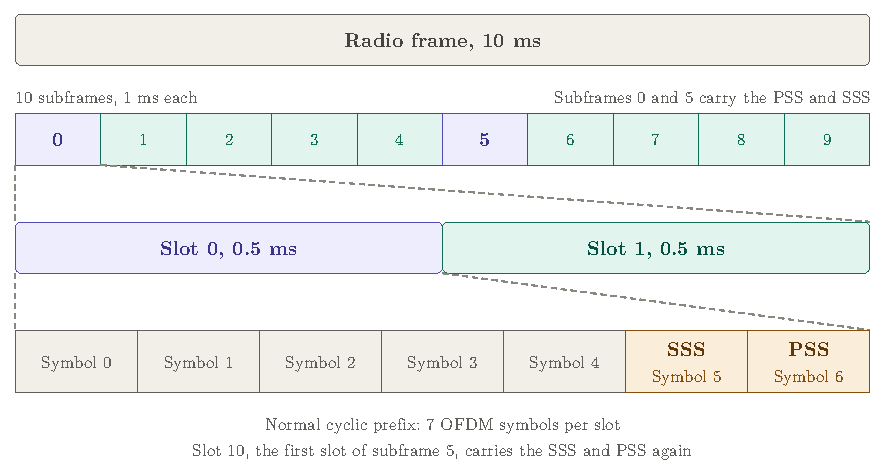
\includegraphics[width=\textwidth]{fig2-lte-frame-sync}
  \caption[Frame structure of the LTE FDD downlink]{Frame structure of the LTE FDD downlink (frame structure type~1) with the normal cyclic prefix. Subframes 0 and 5 carry the secondary and primary synchronization signals (SSS and PSS) in the last two OFDM symbols of their first slot. Drawn from the definitions in \textcite[clauses~4.1, 6.11.1.2 and 6.11.2.2; Table~6.2.3-1]{3gpp2026a}.}
  \label{fig:lte-frame}
\end{figure}

\subsection{Channel Bandwidths and Operating Bands}
\label{sec:lte-bands}

An LTE carrier has one of six channel bandwidths, from \qty{1.4}{\mega\hertz} to \qty{20}{\mega\hertz}, each with a fixed number of resource blocks, its transmission bandwidth configuration \parencite[Table~5.6-1]{3gpp2026b}. Because a resource block is \qty{180}{\kilo\hertz} wide, the resource blocks of a carrier occupy slightly less than its nominal channel bandwidth (\cref{tab:lte-bandwidths}). The receiver used in this study observes at most about \qty{2.56}{\mega\hertz} at a time \parencite{rtlsdrblog2024}. Only the smallest channel bandwidth, \qty{1.4}{\mega\hertz}, fits entirely within that window; of every larger carrier, only a slice is observed.

\begin{table}[tbp]
  \centering
  \caption[LTE channel bandwidths and resource blocks]{LTE channel bandwidths, their transmission bandwidth configurations, and the width occupied by the resource blocks. Sources: \textcite[Table~5.6-1]{3gpp2026b}; resource-block width from \textcite[Table~6.2.3-1]{3gpp2026a}; window width from \textcite{rtlsdrblog2024}.}
  \label{tab:lte-bandwidths}
  \begin{tabular}{S[table-format=2.1] S[table-format=3.0] S[table-format=2.2] c}
    \toprule
    {Channel} & {Resource} & {Occupied} & {Within a \qty{2.56}{\mega\hertz}} \\
    {bandwidth (\unit{\mega\hertz})} & {blocks} & {width (\unit{\mega\hertz})} & {window?} \\
    \midrule
     1.4 &   6 &  1.08 & Yes \\
     3   &  15 &  2.70 & No  \\
     5   &  25 &  4.50 & No  \\
    10   &  50 &  9.00 & No  \\
    15   &  75 & 13.50 & No  \\
    20   & 100 & 18.00 & No  \\
    \bottomrule
  \end{tabular}
\end{table}

The same specification defines the operating bands, with paired uplink and downlink ranges for FDD \parencite[Table~5.5-1]{3gpp2026b}. \Cref{tab:lte-bands} lists the downlink ranges of six FDD bands and shows whether each lies within the tuning range of the receiver, which extends to \qty{1.766}{\giga\hertz} \parencite{rtlsdrblog2024}. Bands~5, 8, 20 and~28 can be received; Bands~3 and~7 cannot. The band studied in this thesis is chosen in Chapter~3.

\begin{table}[tbp]
  \centering
  \caption[Downlink ranges of six LTE FDD bands]{Downlink ranges of six LTE FDD operating bands and whether each lies within the tuning range of the RTL-SDR Blog V4 (\qtyrange{0.5}{1766}{\mega\hertz}). Sources: \textcite[Table~5.5-1]{3gpp2026b}; \textcite{rtlsdrblog2024}.}
  \label{tab:lte-bands}
  \begin{tabular}{l c c}
    \toprule
    Band & Downlink range (\unit{\mega\hertz}) & Within the receiver's range? \\
    \midrule
    28 & \numrange{758}{803}   & Yes \\
    20 & \numrange{791}{821}   & Yes \\
    5  & \numrange{869}{894}   & Yes \\
    8  & \numrange{925}{960}   & Yes \\
    3  & \numrange{1805}{1880} & No  \\
    7  & \numrange{2620}{2690} & No  \\
    \bottomrule
  \end{tabular}
\end{table}

\subsection{Synchronization and Reference Signals}
\label{sec:lte-sync}

Every LTE cell transmits two synchronization signals, which a terminal uses to find the cell and its timing. There are 504 physical-layer cell identities, grouped into 168 cell-identity groups of three identities each; the primary synchronization signal (PSS) is generated from the identity within the group and the secondary synchronization signal (SSS) from the group \parencite[clauses~6.11, 6.11.1.1 and 6.11.2.1]{3gpp2026a}. The PSS is a frequency-domain Zadoff--Chu sequence of length~62. In FDD it is mapped to the last OFDM symbol of slots 0 and~10, that is, once every \qty{5}{\milli\second} \parencite[clauses~6.11.1.1 and 6.11.1.2]{3gpp2026a}. The SSS, an interleaved concatenation of two binary sequences of length~31, occupies the symbol before the PSS in the same slots \parencite[clauses~6.11.2.1 and 6.11.2.2]{3gpp2026a}. Both signals are mapped to the 62 subcarriers around the centre of the carrier, and the five subcarriers on each side are reserved and left empty. The two signals therefore occupy the central 72 subcarriers, six resource blocks or \qty{1.08}{\mega\hertz}, whatever the channel bandwidth \parencite[clauses~6.11.1.2 and 6.11.2.2]{3gpp2026a}.

A cell also transmits cell-specific reference signals (CRS). A terminal may assume that they are transmitted in all downlink subframes of an FDD cell that supports downlink data transmission \parencite[clause~6.10.1]{3gpp2026a}. In subframes configured for multicast and broadcast transmission (MBSFN subframes), they are transmitted only in the first one or two OFDM symbols \parencite[clauses~6.1 and 6.10.1.2]{3gpp2026a}.

Two consequences follow for this study. First, an active LTE carrier is never silent: even with no user traffic, its reference signals are transmitted in every downlink subframe and its synchronization signals every \qty{5}{\milli\second}. Occupancy in this thesis therefore means the presence of a carrier in the observed slice, not the traffic it carries, and idle reference data cannot be taken from quiet periods of an active carrier (Chapter~3). Second, the synchronization signals are confined to the central \qty{1.08}{\mega\hertz} of a carrier, while the receiver observes at most about \qty{2.56}{\mega\hertz}, less than the occupied width of any carrier of \qty{3}{\mega\hertz} or more (\cref{tab:lte-bandwidths}). A window centred on a carrier contains both synchronization signals, but a window placed elsewhere on the carrier contains neither (\cref{fig:obs-window}). A detector that relies on the synchronization signals, such as the correlator reviewed in \cref{sec:waveform}, can therefore work only when the window covers the centre of the carrier. Detectors based on energy, or on the spectrogram as a whole, can respond to any part of it.

\begin{figure}[tbp]
  \centering
  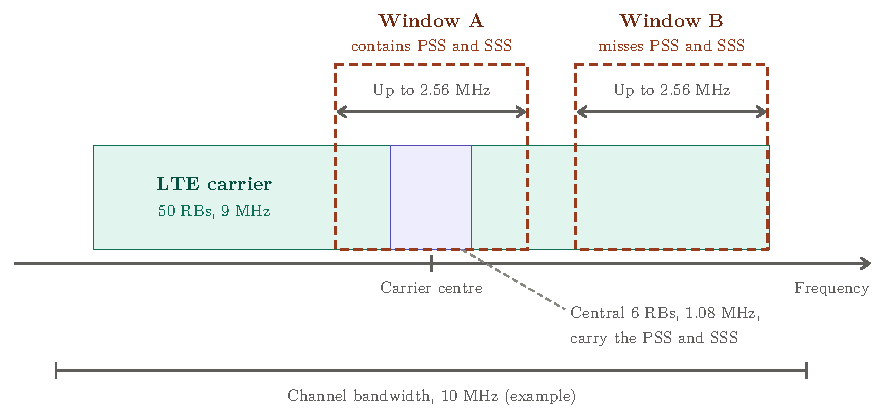
\includegraphics[width=\textwidth]{fig2-observation-window}
  \caption[Receiver window and an LTE carrier]{An example \qty{10}{\mega\hertz} LTE carrier (50 resource blocks, \qty{9}{\mega\hertz} occupied) and two receiver windows of up to \qty{2.56}{\mega\hertz}, drawn to scale in frequency. Window~A, centred on the carrier, contains the PSS and SSS, which occupy the central six resource blocks; window~B, placed off-centre, contains neither. Based on \textcite[Table~5.6-1]{3gpp2026b}, \textcite[Table~6.2.3-1 and clause~6.11]{3gpp2026a} and \textcite{rtlsdrblog2024}.}
  \label{fig:obs-window}
\end{figure}

\section{Cognitive Radio and Dynamic Spectrum Access}
\label{sec:cr}

The term \emph{cognitive radio} was coined by Joseph Mitola \parencite[p.~203]{haykin2005}. \Textcite{mitola1999} described cognitive radio as an extension of software radio with model-based reasoning about radio etiquette, the set of radio frequency bands, air interfaces, protocols, and spatial and temporal patterns that moderate the use of the spectrum (p.~13). They regarded software radio as an ideal platform for cognitive radio (p.~13). The radio's behaviour was organized as a cognition cycle in which it observes its environment, orients itself, plans, decides and acts, with some forms of supervised and unsupervised learning (p.~18).

\Textcite{haykin2005} defined cognitive radio as an intelligent wireless communication system, built on a software-defined radio (SDR), that is aware of its environment, learns from it and adapts to statistical variations in the incoming radio frequency stimuli. It has two objectives: highly reliable communication whenever and wherever needed, and efficient use of the radio spectrum (p.~201). Haykin motivated the concept with measurements showing that some frequency bands are largely unoccupied most of the time, others are partially occupied, and the rest are heavily used (p.~201). This underutilization leads to the notion of a spectrum hole, which he defined as \enquote{a band of frequencies assigned to a primary user, but, at a particular time and specific geographic location, the band is not being utilized by that user} \parencite[p.~201]{haykin2005}. Spectrum utilization could be improved by allowing a secondary user, one not being served in the band, to access a spectrum hole at the right location and time (p.~201). \Cref{fig:spectrum-holes} illustrates the idea.

\begin{figure}[tbp]
  \centering
  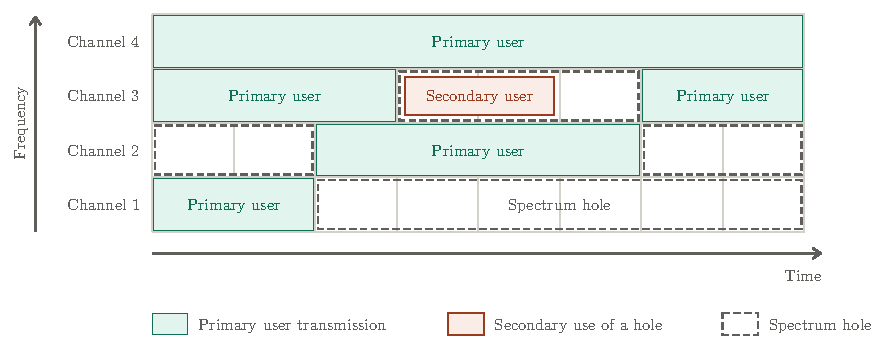
\includegraphics[width=\textwidth]{fig2-spectrum-holes}
  \caption[Spectrum holes in time and frequency]{Spectrum holes in time and frequency at one location (schematic, not to scale). Shaded cells are used by their primary users; an unused cell is a spectrum hole, which a secondary user may occupy until the primary user returns. Drawn after the definition of \textcite[p.~201]{haykin2005}.}
  \label{fig:spectrum-holes}
\end{figure}

Haykin identified three fundamental cognitive tasks: radio-scene analysis, which includes the detection of spectrum holes; channel identification; and transmit-power control with dynamic spectrum management. The first two are carried out in the receiver and the third in the transmitter \parencite[p.~202]{haykin2005}. He also classified the spectrum by measured power into black spaces, occupied by high-power local interferers some of the time; grey spaces, partially occupied by low-power interferers; and white spaces, free of radio frequency interferers except for ambient natural and artificial noise. White spaces, and grey spaces to a lesser extent, are the candidates for secondary use (p.~206).

Spectrum sensing is the function through which a cognitive radio finds these opportunities, and \textcite{yucek2009} described it as one of the most challenging issues in cognitive radio systems (p.~116). The motivation for cognitive radio comes from measurements showing unused resources in frequency, time and space, but cognitive radios must be able to detect very weak primary signals \parencite[pp.~322--323]{axell2010}, because the primary users must be detected in order to avoid causing them harmful interference \parencite{tandra2008}. In Nigeria, \textcite{popoola2018} measured an average occupancy below \pct{10} over \qtyrange{80}{2200}{\mega\hertz} at five sites, and concluded that dynamic spectrum access has a hopeful future in the country (Chapter~1).

This thesis does not build a cognitive radio. It addresses the sensing step on which cognitive radio, and spectrum monitoring generally, depend: deciding whether an LTE carrier is present in an observed slice of spectrum. A band that holds an active LTE carrier offers no opportunity to a secondary user at that place and time; it becomes a spectrum hole only where and when the carrier is absent.

\section{Classical Spectrum Sensing}
\label{sec:sensing}

\subsection{The Detection Problem}
\label{sec:detection-problem}

Spectrum sensing is posed as a binary hypothesis test. Let $y(n)$, $n = 0, \dots, N-1$, be the complex baseband samples observed in one sensing interval. Under the null hypothesis $\mathcal{H}_0$ the band holds noise only; under the alternative $\mathcal{H}_1$ a signal is present \parencite[p.~322]{axell2010}:
\begin{align}
  \mathcal{H}_0 &: \quad y(n) = w(n), \label{eq:h0}\\
  \mathcal{H}_1 &: \quad y(n) = s(n) + w(n), \label{eq:h1}
\end{align}
where $s(n)$ is the signal and $w(n)$ is noise, commonly modelled as independent, zero-mean, circularly symmetric complex Gaussian samples with variance $\sigma^2$ \parencite[p.~322]{axell2010}. A detector computes a test statistic $T$ from the samples and decides $\mathcal{H}_1$ when $T$ exceeds a threshold $\lambda$. Its performance is summarized by two probabilities \parencite[p.~121]{yucek2009}: the probability of detection, $\Pd = \Pr(T > \lambda \mid \mathcal{H}_1)$, and the probability of false alarm, $\Pfa = \Pr(T > \lambda \mid \mathcal{H}_0)$. A high $\Pd$ is wanted, and $\Pfa$ should be kept small so that transmission opportunities are not wasted (p.~121).

The threshold trades $\Pd$ against $\Pfa$. The signal power is difficult to know, since it depends on the transmission and on the distance to the transmitter, so in practice the threshold is chosen to obtain a given false-alarm rate, for which knowledge of the noise variance suffices \parencite[p.~121]{yucek2009}. This is the Neyman--Pearson approach: for a fixed $\Pfa$, the optimal test compares the log-likelihood ratio with a threshold \parencite[p.~322]{axell2010}. The detectors in this thesis are compared in the same way. Each threshold is set on idle validation data for a fixed $\Pfa$ of \pct{1} or \pct{5}, and $\Pd$ is measured at that operating point (Chapter~3).

\subsection{A Taxonomy of Sensing Methods}
\label{sec:taxonomy}

Sensing methods differ mainly in how much they must know about the signal to be detected. \Textcite{yucek2009} reviewed energy detection, waveform-based sensing, cyclostationarity-based sensing, radio identification, matched filtering and other methods such as multitaper and wavelet-based spectral estimation, and compared the main methods by accuracy and complexity (pp.~120--124). Energy detection needs no knowledge of the primary signal, whereas matched filtering needs complete knowledge of it (pp.~120, 123). \Textcite{axell2010} likewise distinguished the energy detector, which assumes no known structure in the signal, from feature detectors that exploit known structure, such as cyclostationarity or the eigenvalue structure of the signal covariance matrix (pp.~322--324). Cooperation among several sensors has been proposed as a remedy for noise uncertainty, fading and shadowing \parencite[p.~124]{yucek2009}; it is outside the scope of this single-receiver study.

\Cref{fig:taxonomy} arranges five non-cooperative methods by the prior knowledge each requires, and \cref{tab:sensing-methods} compares them. Learned detectors, which derive their decision rule from data rather than from a signal model, are shown as a separate branch and are reviewed in \cref{sec:ae,sec:related}. Energy detection, the core baseline of this thesis, is reviewed in the most detail.

\begin{figure}[tbp]
  \centering
  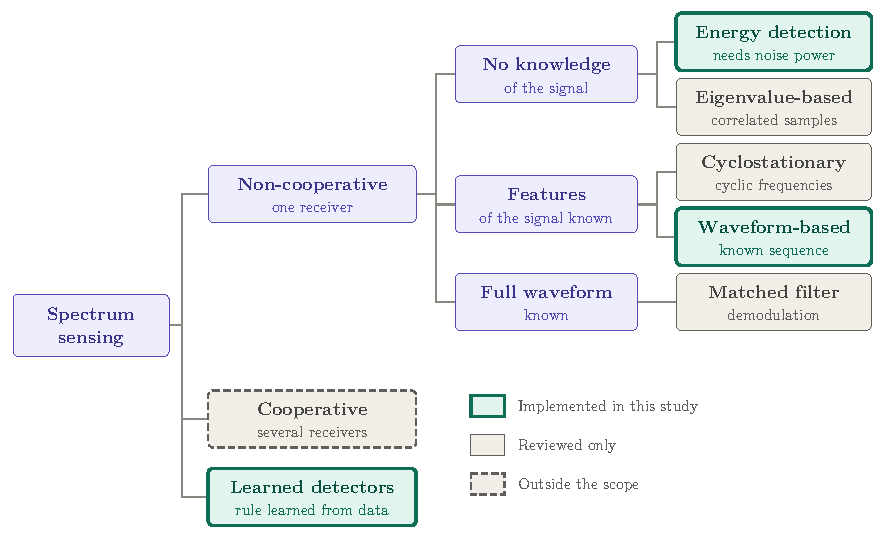
\includegraphics[width=\textwidth]{fig2-sensing-taxonomy}
  \caption[Taxonomy of spectrum sensing methods]{Spectrum sensing methods arranged by the prior knowledge they require. Cooperative sensing is outside the scope of this study; learned detectors are reviewed in \cref{sec:ae,sec:related}. Based on \textcite{yucek2009}, \textcite{axell2010} and \textcite{zeng2009}.}
  \label{fig:taxonomy}
\end{figure}

\begin{table}[tbp]
  \centering
  \small
  \caption[Classical spectrum sensing methods compared]{Classical spectrum sensing methods compared. Sources: \textcite[pp.~120--124]{yucek2009}; \textcite[pp.~322--324]{axell2010}; \textcite{zeng2009}; \textcite{tandra2008}.}
  \label{tab:sensing-methods}
  \begin{tabularx}{\textwidth}{@{} >{\raggedright\arraybackslash}p{2.7cm} >{\raggedright\arraybackslash}X >{\raggedright\arraybackslash}X >{\raggedright\arraybackslash}X @{}}
    \toprule
    Method & Prior knowledge needed & Strengths & Limitations \\
    \midrule
    Energy detection & None about the signal; the noise power, to set the threshold & Simple; low computational and implementation cost; detects any type of signal & Cannot tell primary signals from interference or noise; poor at low signal-to-noise ratio (SNR); SNR wall under noise uncertainty \\
    \addlinespace
    Matched filtering & The complete waveform: bandwidth, frequency, modulation, pulse shaping and frame format; demodulation & Optimal when the signal is known; short sensing time for a given $\Pfa$ & A receiver for every signal type; high complexity and power consumption; SNR wall when channel coherence times are finite \\
    \addlinespace
    Cyclostationary detection & The cyclic frequencies of the signal & Distinguishes noise from modulated signals and different signal types from each other & Worse than energy detection in stationary noise; features can be lost in fading; SNR wall under model uncertainty; sensitive to sampling-clock offsets \\
    \addlinespace
    Eigenvalue-based detection & None about the signal, the channel or the noise power; correlated signal samples & Overcomes noise uncertainty; can beat ideal energy detection for highly correlated signals & A sample covariance matrix and its eigenvalues are needed for every decision \\
    \addlinespace
    Waveform-based detection & A known pattern in the signal: preamble, pilot or synchronization sequence & More reliable and faster to converge than energy detection; improves with pattern length & Applies only to signals with known patterns; susceptible to synchronization errors \\
    \bottomrule
  \end{tabularx}
\end{table}

\subsection{Energy Detection}
\label{sec:ed}

Energy detection is the classical way to detect a signal of unknown form. In the classic analysis by Urkowitz, a deterministic signal of unknown structure is detected in flat, band-limited Gaussian noise of known power spectral density. The received signal is passed through an ideal band-pass filter, its energy over an interval is measured, and the energy is compared with a threshold; the decision statistic then has a noncentral chi-square distribution \parencite[Urkowitz, 1967, as cited in][p.~1606]{kostylev2002}. Received signals often have a random amplitude because of fading, in which case the statistic is no longer chi-square distributed, and \textcite{kostylev2002} derived the detection probability for Rayleigh, Rice, Nakagami and other amplitude distributions (p.~1606). \Cref{fig:ed-block} shows the detector in its sampled form, which is the form used in this thesis.

\begin{figure}[tbp]
  \centering
  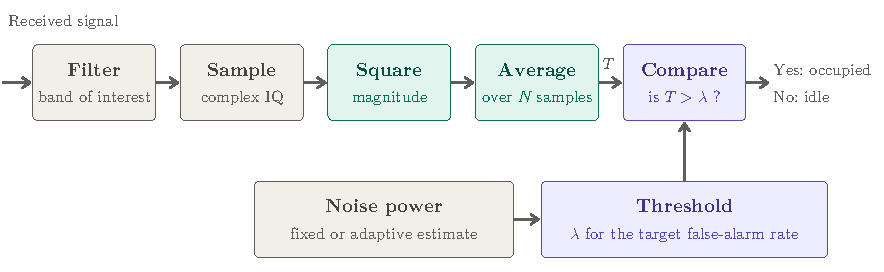
\includegraphics[width=\textwidth]{fig2-energy-detector}
  \caption[Block diagram of the energy detector]{Block diagram of the energy detector in sampled form. The received signal is band-limited and sampled, the squared magnitudes of $N$ samples are averaged, and the average is compared with a threshold $\lambda$ set from the noise power for a target $\Pfa$. Based on \textcite{kostylev2002}, \textcite{axell2010} and \textcite{yucek2009}.}
  \label{fig:ed-block}
\end{figure}

In discrete time, the detector computes the average power of the $N$ samples,
\begin{equation}
  T = \frac{1}{N} \sum_{n=0}^{N-1} \lvert y(n) \rvert^2 ,
  \label{eq:ed-statistic}
\end{equation}
and decides $\mathcal{H}_1$ if $T > \lambda$ \parencite[p.~322]{axell2010}; \textcite{yucek2009} used the same statistic without the factor $1/N$ (p.~121). If the signal is also modelled as zero-mean complex Gaussian, with variance $\sigma_s^2$, the energy detector is the optimal detector in the Neyman--Pearson sense \parencite[p.~322]{axell2010}. The sum $NT$ then follows a scaled chi-square distribution with $2N$ degrees of freedom under both hypotheses, scaled by $\sigma^2/2$ under $\mathcal{H}_0$ and by $(\sigma^2 + \sigma_s^2)/2$ under $\mathcal{H}_1$ \parencite[p.~121]{yucek2009}. Writing $F_{\chi^2_{2N}}$ for the cumulative distribution function of a chi-square variable with $2N$ degrees of freedom, the false-alarm and detection probabilities of \cref{eq:ed-statistic} are
\begin{equation}
  \Pfa = 1 - F_{\chi^2_{2N}}\!\left( \frac{2N\lambda}{\sigma^2} \right), \qquad
  \Pd = 1 - F_{\chi^2_{2N}}\!\left( \frac{2N\lambda}{\sigma^2 + \sigma_s^2} \right),
  \label{eq:ed-pfa-pd}
\end{equation}
and the threshold for a target $\Pfa$ is
\begin{equation}
  \lambda = \frac{\sigma^2}{2N}\, F^{-1}_{\chi^2_{2N}}\!\left(1 - \Pfa\right),
  \label{eq:ed-threshold}
\end{equation}
which follow from the expressions of \textcite[p.~323]{axell2010} for the unnormalized statistic. The SNR is $\gamma = \sigma_s^2/\sigma^2$ \parencite[p.~121]{yucek2009}.

\Cref{eq:ed-threshold} shows the defining property of the method: the threshold depends on the noise variance and not on the signal. Energy detection is universal in the sense that it can detect any type of signal without knowing anything about it, but for the same reason it cannot exploit any knowledge that is available, and it needs the noise power to set its threshold \parencite[p.~323]{axell2010}. \Textcite{yucek2009} described it as the most common way of spectrum sensing because of its low computational and implementation complexity. They listed its main challenges as the selection of the threshold, the inability to tell primary users from interference and noise, and poor performance at low SNR (pp.~120--121). Its performance is also limited when the noise is not stationary or its variance is not known (p.~124).

The noise power is never known exactly. \Textcite{zeng2009} distinguished receiver device noise uncertainty, which arises from the non-linearity of components and from thermal noise that is non-uniform and time-varying, from environmental noise uncertainty, which is caused by other transmissions; because of noise uncertainty, an accurate noise power is very difficult to obtain in practice. A small error in the noise-power estimate causes a significant loss of performance \parencite[p.~121]{yucek2009}. \Textcite{tandra2008} made this precise. They modelled the noise power as known only to lie in an interval $[\sigma_n^2/\rho,\ \rho\,\sigma_n^2]$ around a nominal value $\sigma_n^2$, where $\rho = 10^{\delta/10}$ for an uncertainty of $\delta$ decibels. The energy detector then cannot robustly detect a signal whose power is smaller than the width of that interval, $(\rho - 1/\rho)\,\sigma_n^2$. The result is an \emph{SNR wall},
\begin{equation}
  \mathrm{SNR}_{\mathrm{wall}} = \frac{\rho^2 - 1}{\rho},
  \label{eq:snr-wall}
\end{equation}
below which a detector cannot robustly achieve a useful pair of $\Pfa$ and $\Pd$, however long it observes the channel. An uncertainty of \qty{1}{\decibel}, for example, gives a wall at about \qty{-3.3}{\decibel}, and the number of samples needed grows without bound as the SNR approaches the wall. \Cref{fig:ed-pd-snr} illustrates the effect. Tandra and Sahai further proved that, when the modulation of the signal is unknown, every detector has an SNR wall, and any detector is essentially as non-robust as the energy detector. \Textcite[p.~323]{axell2010} noted that the result was later extended to other model uncertainties, including non-white or non-stationary noise, flat fading, non-ideal filters and finite-precision analogue-to-digital converters, and that noise calibration improves robustness. A related limit comes from the receiver's finite dynamic range. If a radio can quantize voltages only between upper and lower limits, any detector can be rendered useless at low enough SNR, even under moderate noise uncertainty, and all physical radios have such a limit \parencite{tandra2005}. The 8-bit converter of the receiver used here makes this limit concrete (\cref{sec:sdr}).

\begin{figure}[tbp]
  \centering
  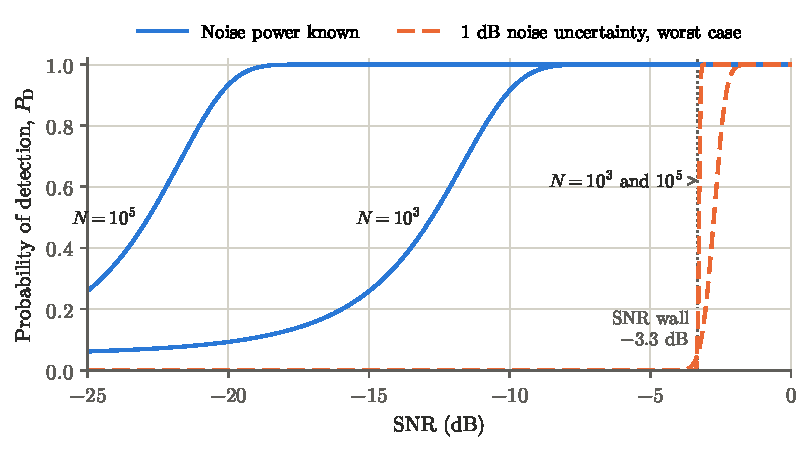
\includegraphics[width=\textwidth]{fig2-ed-pd-snr}
  \caption[Energy detector: detection probability against SNR]{Probability of detection of the energy detector against SNR at $\Pfa = 0.05$, for $N = 10^3$ and $N = 10^5$ complex samples. Solid lines: noise power known exactly, from \cref{eq:ed-pfa-pd,eq:ed-threshold}. Dashed lines: \qty{1}{\decibel} of noise uncertainty, worst case, with the threshold set for the highest noise power in the uncertainty interval and $\Pd$ evaluated at the lowest, following \textcite{tandra2008}. The dotted line marks the SNR wall of \cref{eq:snr-wall}. Analytic curves, not measurements.}
  \label{fig:ed-pd-snr}
\end{figure}

Because its threshold must follow the noise power, a practical energy detector estimates that power. \Textcite{yucek2009} described methods that estimate the noise level dynamically, for example as the smallest eigenvalue of the autocorrelation of the received signal, and then use the estimate to set the threshold for a constant false-alarm rate (CFAR); other methods find the threshold iteratively for a given $\Pfa$ (p.~121). In spectrum occupancy campaigns, measured power levels are compared with pre-established thresholds, which is energy detection in its simplest form \parencite[p.~35]{reyesmoncayo2018}. This thesis uses two variants (Chapter~3). The fixed-threshold detector freezes its noise estimate at calibration. The adaptive detector updates its estimate from recent frames judged idle, and so follows the CFAR principle. Detectors that estimate the noise from neighbouring frequency or time cells, which are often called CFAR detectors, are not implemented (Chapter~1). How the threshold of the energy detector is set also matters when it is used as a baseline for learned detectors, a point taken up in \cref{sec:related-ed}.

\subsection{Matched-Filter Detection}
\label{sec:mf}

If the signal to be detected is perfectly known, the optimal detector is a matched filter \parencite[p.~323]{axell2010}. Its main advantage is the short time it needs to reach a given probability of false alarm or of missed detection \parencite[p.~123]{yucek2009}. It requires, however, that the cognitive radio demodulate the received signal, and hence perfect knowledge of the primary user's signalling features, such as bandwidth, operating frequency, modulation type and order, pulse shaping and frame format. Since a receiver is needed for every signal type, the sensing unit becomes impractically complex, and executing the receiver algorithms consumes much power (p.~123). Coherent detection is not immune to model uncertainty either: with finite channel coherence times it also has an SNR wall, although one that scales more favourably with coherence time than that of cyclostationary detectors \parencite{tandra2008}. Demodulation of LTE is outside the scope of this study (Chapter~1), so the matched filter is not used. Its partial form, correlation with known synchronization sequences, is discussed in \cref{sec:waveform}.

\subsection{Cyclostationary Feature Detection}
\label{sec:cyclo}

Most man-made signals show periodic patterns related to the symbol rate, chip rate, channel code or cyclic prefix. They can be modelled as cyclostationary random processes, whose covariance is periodic in time \parencite[p.~323]{axell2010}. Cyclostationary detectors use the cyclic correlation function of the received signal instead of its power spectral density. Because noise is wide-sense stationary with no correlation while modulated signals are cyclostationary, these detectors can distinguish noise from primary signals, and can also distinguish different types of transmission \parencite[p.~122]{yucek2009}. OFDM signals, used by WiFi, WiMAX, LTE and digital television, have well-known spectral correlation properties, which has made their cyclostationary detection a subject of considerable interest \parencite[p.~323]{axell2010}. The method has costs. Cyclostationary detectors perform worse than energy detectors when the noise is stationary, although they are unaffected by the non-stationary noise caused by co-channel or adjacent-channel interferers, which defeats energy detectors. Their features can be lost through channel fading, model uncertainties cause an SNR wall for them as for energy detectors, and they are vulnerable to sampling-clock offsets \parencite[p.~124]{yucek2009}. They also require the cyclic frequencies of the primary signal \parencite{zeng2009}. They are not implemented in this study.

\subsection{Eigenvalue-Based Detection}
\label{sec:eigen}

Eigenvalue-based detectors exploit the structure of the covariance matrix of the received samples. Under $\mathcal{H}_0$, with white noise, all its eigenvalues equal $\sigma^2$. Under $\mathcal{H}_1$ the eigenvalues of a correlated signal are added to them, so the largest eigenvalues differ markedly from the smallest \parencite[p.~324]{axell2010}. \Textcite{zeng2009} proposed two tests on the sample covariance matrix, the ratio of the maximum to the minimum eigenvalue and the ratio of the average to the minimum eigenvalue, and used random matrix theory to set their thresholds for a given $\Pfa$. Their methods need no knowledge of the signal, the channel or the noise power. They overcome the noise-uncertainty problem and can perform better than an ideal energy detector when the signal samples are highly correlated; energy detection, by contrast, is optimal for independent and identically distributed signals but not for correlated ones. Each decision requires a sample covariance matrix, built from a number of consecutive samples called the smoothing factor, and its extreme eigenvalues. Eigenvalue-based detectors are not implemented in this study.

\subsection{Waveform-Based Detection}
\label{sec:waveform}

Wireless systems often transmit known patterns, such as preambles, midambles, regularly transmitted pilots and spreading sequences, to assist synchronization. Correlating the received signal with a known copy of such a pattern is called waveform-based, or coherent, sensing, and it applies only to systems with known signal patterns \parencite[p.~122]{yucek2009}. \Textcite{yucek2009} reported that it outperforms energy detection in reliability and convergence time, that its performance improves as the known pattern grows longer, and that it needs only short measurements but is susceptible to synchronization errors (p.~122). Because of its coherent processing it is more robust than energy and cyclostationary detection, but it requires a priori knowledge of the primary signal (pp.~123--124).

The LTE PSS and SSS (\cref{sec:lte-sync}) are such patterns. A correlator that searches the observed window for the known synchronization sequences is an instance of waveform-based sensing, and it is included in this study as a baseline (Chapter~3). Because the synchronization signals occupy only the central \qty{1.08}{\mega\hertz} of a carrier, such a correlator can detect a carrier only when the receiver's window covers the carrier's centre (\cref{fig:obs-window}). LTE synchronization signals have also served a different purpose with low-cost receivers: \textcite{calvopalomino2017} used them as a reference for estimating the frequency offset of the local oscillator in RTL-SDR devices (\cref{sec:sdr}).

\section{Software-Defined Radio and the RTL-SDR}
\label{sec:sdr}

A software-defined radio performs in software much of the signal processing that conventional radios perform in dedicated hardware. \Textcite{haykin2005} attributed its practical reality to the convergence of digital radio and computer software, and noted that the term was also coined by Mitola (pp.~202--203). Cognitive radio relies on software-defined radio for reconfigurability (p.~202), and \textcite{mitola1999} regarded software radio as the platform on which cognitive radio would be built (p.~13). For spectrum measurement, the appeal of SDR is that one inexpensive receiver can be retuned and reprogrammed in software for different bands and processing chains.

The RTL-SDR is the cheapest widely used example. RTL-SDR dongles were designed for the reception of digital television (DVB-T), and were found by hardware hackers to be usable as general-purpose SDRs \parencite[p.~1]{rtlsdrblog2024}. \Textcite{calvopalomino2017} attributed their popularity among academics and hobbyists to their very low price (below 25 US dollars), ease of use and the wide availability of open-source SDR software. This study uses the RTL-SDR Blog V4, a version redesigned for SDR use; its specifications are listed in \cref{tab:rtlsdr-v4}. The V4 uses the R828D tuner, whose three inputs are fed by a triplexer that splits the antenna input into high-frequency, very-high-frequency and ultra-high-frequency bands. Simple notch filters for the broadcast AM, FM and digital audio broadcasting (DAB) bands attenuate those signals by a few decibels \parencite[p.~1]{rtlsdrblog2024}.

\begin{table}[tbp]
  \centering
  \caption[Specifications of the RTL-SDR Blog V4]{Specifications of the RTL-SDR Blog V4 relevant to this study. Source: \textcite[p.~1]{rtlsdrblog2024}.}
  \label{tab:rtlsdr-v4}
  \begin{tabularx}{\textwidth}{@{} l >{\raggedright\arraybackslash}X @{}}
    \toprule
    Parameter & Value \\
    \midrule
    Tuner & Rafael Micro R828D \\
    Analogue-to-digital converter & Realtek RTL2832U, 8 bits \\
    Frequency range & \qty{500}{\kilo\hertz} to \qty{1.766}{\giga\hertz} \\
    Bandwidth & \qty{2.56}{\mega\hertz} stable (up to \qty{3.2}{\mega\hertz} with dropped samples) \\
    Input impedance & \qty{50}{\ohm} (typical) \\
    Reference oscillator & Temperature-compensated crystal oscillator (TCXO), \qty{1}{ppm} \\
    Bias tee & \qty{4.5}{\volt}, \qty{180}{\milli\ampere}, switchable in software \\
    Front end & Triplexer with switchable notch filters \\
    Connectors & SMA (antenna); USB-A (host) \\
    Transmit capability & None \\
    \bottomrule
  \end{tabularx}
\end{table}

The internal architecture of the RTL-SDR is not fully documented. \Textcite{calvopalomino2017} therefore modelled it as a generic receiver in which a single local oscillator feeds both the down-conversion stage and the sampling stage, which converts the in-phase and quadrature (IQ) components to digital samples. \Cref{fig:rtlsdr-chain} shows the receive chain used in this study at that functional level. The dongle delivers complex IQ samples over the universal serial bus (USB) to the host, where all further processing takes place in software \parencite{calvopalomino2015}.

\begin{figure}[tbp]
  \centering
  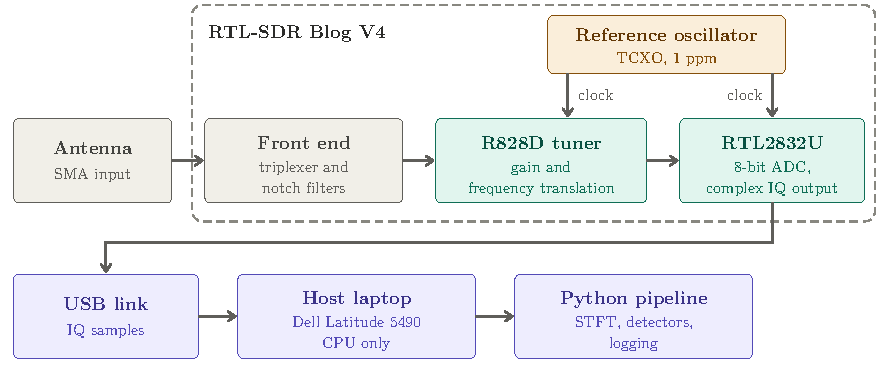
\includegraphics[width=\textwidth]{fig2-rtlsdr-chain}
  \caption[Receive chain of the RTL-SDR and host laptop]{Functional receive chain of the RTL-SDR Blog V4 and the host laptop. The tuner translates the selected band to an intermediate frequency; the RTL2832U digitizes it with an 8-bit converter and delivers complex IQ samples over USB. One reference oscillator clocks both the frequency translation and the sampling. Functional view only: the chips' internal design is not fully documented. Based on \textcite[p.~1]{rtlsdrblog2024} and the receiver model of \textcite{calvopalomino2017}.}
  \label{fig:rtlsdr-chain}
\end{figure}

Low-cost receivers have made continuous and distributed spectrum measurement affordable. \Textcite{calvopalomino2015} demonstrated a sensor platform for large-scale wideband monitoring built from a single-board computer and an RTL-SDR dongle, which scanned the spectrum in steps of \qty{2.4}{\mega\hertz}, the bandwidth sensed at a time with 8-bit resolution. Electrosense extended this approach to a crowdsourced network of low-cost sensors, motivated by how little is known about the actual use of the spectrum over time and space, and made the collected spectrum data available as an open service \parencite{rajendran2018}. Electrosense+ moved the decoding of signals onto the sensors themselves, which used RTL-SDR receivers with temperature-compensated oscillators and sent no raw IQ data to users \parencite{calvopalomino2020}. \Textcite{reyesmoncayo2018} built a low-cost monitor of channel occupancy from an embedded board, Python and an RTL-SDR dongle, noting that the equipment used in earlier occupancy campaigns was too costly for continuous monitoring in many places (p.~34). \Textcite{molinatenorio2021} linked several affordable SDRs, including an RTL-SDR, to sense a wide band in real time with a detector based on wavelets, machine learning and the Higuchi fractal dimension, and reported a \pct{95} probability of success at SNRs above \qty{0}{\decibel} (p.~1). \Textcite{saber2021} used an RTL-SDR to capture real signals for a deep-learning detector (\cref{sec:related-ed}).

Low cost comes with imperfections that a detector must tolerate.
\begin{itemize}
  \item \emph{Frequency offset.} In the dongle used by \textcite{calvopalomino2015}, the oscillator had inaccuracies of the order of \qty{50}{ppm}, which appeared as a temperature-dependent frequency error of a few kilohertz. Using the LTE synchronization signals as a reference, \textcite{calvopalomino2017} found that RTL-SDR models fitted with a temperature-compensated oscillator stayed well within their specified tolerance of \qty{1}{ppm}. The V4 has such an oscillator (\cref{tab:rtlsdr-v4}).
  \item \emph{The direct-current (DC) component.} The processing chain of \textcite{calvopalomino2015} included a DC-removal step before windowing and the fast Fourier transform (FFT).
  \item \emph{Finite dynamic range.} The 8-bit converter limits the range of signal levels that can be represented at once, and a finite dynamic range sets a hard limit on detection at low SNR \parencite{tandra2005}.
  \item \emph{Gain.} The tuner gain is set in software and changes the level of the recorded noise floor, so it is fixed within each capture session and logged (Chapter~3).
\end{itemize}

\section{Time--Frequency Representation}
\label{sec:stft}

An LTE carrier has structure in both time and frequency: its resource blocks occupy contiguous subcarriers, and its synchronization and reference signals recur at fixed intervals (\cref{sec:lte}). The energy statistic of \cref{eq:ed-statistic} discards this structure by summing over the whole observation. A time--frequency representation keeps it, and is the input to the learned detectors in this study.

The short-time Fourier transform (STFT) is the standard such representation. \Textcite{allen1977} defined it as
\begin{equation}
  X_n(e^{j\omega}) = \sum_{m=-\infty}^{\infty} y(m)\, h(n - m)\, e^{-j\omega m},
  \label{eq:stft}
\end{equation}
where the window $h$ selects the portion of the signal $y$ being analysed around time $n$ (p.~1558; their notation adapted). In practice the transform is evaluated at $K$ uniformly spaced frequencies and at frames spaced $R$ samples apart. For complex samples $y(n)$ at a sampling rate $f_s$, frame $\ell$ and frequency bin $k$ give
\begin{equation}
  X(\ell, k) = \sum_{m=0}^{L-1} h(m)\, y(\ell R + m)\, e^{-j 2\pi k m / K}, \qquad k = 0, \dots, K-1,
  \label{eq:stft-discrete}
\end{equation}
with a window of $L$ samples, a bin spacing of $f_s/K$ and a frame spacing of $R/f_s$ seconds. The spectrogram is the squared magnitude, usually in decibels, $S(\ell, k) = 10 \log_{10} \lvert X(\ell, k) \rvert^2$. Arranged over consecutive frames, it forms an image with time along one axis and frequency along the other (\cref{fig:stft}).

\begin{figure}[tbp]
  \centering
  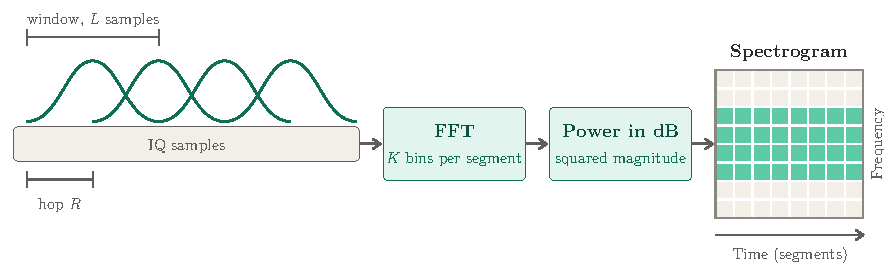
\includegraphics[width=\textwidth]{fig2-stft-spectrogram}
  \caption[From IQ samples to a spectrogram]{From IQ samples to a spectrogram (schematic). Overlapping windowed segments of the IQ stream are transformed with the FFT, and their squared magnitudes in decibels form the columns of a time--frequency image. The shading of the image is illustrative, not data. Based on \textcite{allen1977}.}
  \label{fig:stft}
\end{figure}

Because $X_n$ is the Fourier transform of the product of the signal and the window, it is the convolution of their transforms, so the details of the STFT depend strongly on the window. The window must therefore be chosen to suit the desired time and frequency resolution \parencite[p.~1558]{allen1977}: a long window resolves frequency finely but blurs events in time, and a short window does the reverse (p.~1559). For spectrum displays and signal detection, the STFT serves as a representation of a non-stationary signal and no resynthesis is needed (p.~1559), which is the case in this study.

The shape of the window also matters. A finite record projects any frequency that does not coincide with one of the basis frequencies onto the whole basis set. This spectral leakage results from processing finite-duration records, and windows are weighting functions applied to the data to reduce it \parencite[p.~52]{harris1978}. Windows affect detectability, resolution, dynamic range, confidence and ease of implementation (p.~53). Two of Harris's figures of merit bear directly on detection. The equivalent noise bandwidth of a window is the width of the rectangular filter that has the same peak power gain and accumulates the same noise power; a larger equivalent noise bandwidth admits more noise into each bin and reduces the processing gain (pp.~54, 56). The peak sidelobe level and the rate at which sidelobes fall off indicate how well a window suppresses leakage from strong signals into distant bins (p.~57). For an occupancy detector, leakage from a strong carrier can raise bins outside it, while the equivalent noise bandwidth sets the noise level in each bin, so the window affects both the idle and the occupied statistics.

Spectrograms and averaged power spectra are the usual inputs to learned spectrum detectors. \Textcite[p.~4]{xu2021} and \textcite[p.~4]{tian2022} computed STFT spectrograms of captured IQ data and down-sampled them to $64 \times 64$ images. \Textcite{tandiya2018} used spectrogram images from a waterfall display, and \textcite{rajendran2020} used patches of consecutive power spectral density (PSD) vectors. In this study the spectrogram, or a frame of it, is the input to the autoencoders and to the linear reconstruction baseline of \cref{sec:ae-pca} (Chapter~3).

\section{Autoencoders and Anomaly Detection}
\label{sec:ae}

The autoencoders studied in this thesis are its AI-based detectors. They are neural networks \parencite[p.~499]{goodfellow2016} and therefore belong to machine learning, which is used for many, though not all, approaches to AI \parencite[p.~9]{goodfellow2016}. This section describes how they detect anomalies, how they relate to PCA, the architectures compared, the variational autoencoder, and how their thresholds are set.

\subsection{Anomaly Detection with Normal-Only Training}
\label{sec:ae-anomaly}

An anomaly is an observation that deviates considerably from some concept of normality \parencite{ruff2021}. In the unsupervised setting, a model is trained on unlabelled data that are assumed to be drawn from the normal distribution; such training data are called clean, although in practice they may contain noise or contamination \parencite{ruff2021}. Reconstruction-based methods learn a model that reconstructs normal data well, and they detect anomalies by their failure to reconstruct them accurately; they are among the earliest and most common neural approaches to anomaly detection \parencite{ruff2021}.

Most spectrum anomaly detectors treat a band with its usual signals as normal and an unexpected signal as the anomaly (\cref{sec:related-anomaly}). This study inverts that arrangement. Idle spectrum, the receiver noise and whatever the environment contributes in a band without an LTE carrier, is the normal class, and an LTE carrier is the anomaly to be detected. \Textcite{torio2025} framed transmission detection in the same way, assuming that the normal state of a channel is the absence of transmissions (p.~5). A practical consequence is the need for clean idle training data: any LTE energy left in the training frames would be learned as normal, which is why the idle window is surveyed and checked before any idle data are captured (\cref{sec:m-survey}).

\subsection{Principal Component Analysis and the Autoencoder}
\label{sec:ae-pca}

Principal component analysis (PCA) finds an orthogonal basis that maximizes the variance of the centred data. Its components are the eigenvectors of the empirical covariance matrix with the largest eigenvalues. Equivalently, PCA finds the projection onto a $d$-dimensional linear subspace that minimizes the mean squared reconstruction error, and in that form it can be regarded as the default reconstruction baseline for anomaly detection \parencite{ruff2021}. With the $d$ leading eigenvectors as the rows of a $d \times D$ matrix $\mathbf{W}$, the reconstruction error of an input $\mathbf{x}$ is $\lVert \mathbf{x} - \mathbf{W}^{\top}\mathbf{W}\mathbf{x} \rVert^2$.

An autoencoder is a neural network trained to copy its input to its output. It consists of an encoder $\mathbf{h} = f(\mathbf{x})$, which produces a code, and a decoder $\mathbf{r} = g(\mathbf{h})$, which produces a reconstruction, and it is trained to minimize a loss that penalizes the difference between $g(f(\mathbf{x}))$ and $\mathbf{x}$, such as the mean squared error \parencite[pp.~499--500]{goodfellow2016}. When the code has fewer dimensions than the input, the autoencoder is called undercomplete, and it is forced to capture the most salient features of the training data (p.~500). For $n$ training inputs $\mathbf{x}_i$, each with $D$ elements, the training objective is
\begin{equation}
  \min_{f,\, g} \; \frac{1}{n} \sum_{i=1}^{n} \bigl\lVert \mathbf{x}_i - g\bigl(f(\mathbf{x}_i)\bigr) \bigr\rVert^2 ,
  \label{eq:ae-objective}
\end{equation}
and the anomaly score of a new input is its reconstruction error, $e(\mathbf{x}) = \frac{1}{D} \lVert \mathbf{x} - g(f(\mathbf{x})) \rVert^2$, the mean squared error (MSE) over its $D$ elements \parencite{ruff2021}. With a linear decoder and the mean squared error as loss, an undercomplete autoencoder learns the same subspace as PCA; with non-linear encoder and decoder functions it can learn a more powerful, non-linear generalization of PCA \parencite[p.~500]{goodfellow2016}. \Textcite{ruff2021} likewise noted that a linear autoencoder with a bottleneck recovers the subspace spanned by the PCA eigenvectors. PCA is therefore the natural baseline for an autoencoder: if the non-linear model does not detect better than PCA, its extra complexity is not justified. That comparison is part of RQ2.

\subsection{Fully Connected versus Convolutional Architectures}
\label{sec:ae-architectures}

A spectrogram can be fed to an autoencoder in two ways. A fully connected autoencoder flattens it into a vector and uses dense layers, in which every output unit interacts with every input unit through its own parameter. A convolutional autoencoder keeps the two-dimensional layout and uses convolutional layers. \Textcite{goodfellow2016} identified three properties of convolution that help a learning system (pp.~329--334). The first is sparse interactions: the kernel is smaller than the input, so a layer with $m$ inputs and $n$ outputs needs only $k \times n$ parameters for a kernel of $k$ elements instead of $m \times n$. The second is parameter sharing: the same kernel is applied at every position. The third, which follows from parameter sharing, is equivariance to translation: when a pattern in the input shifts, its representation shifts in the same way. \Textcite{masci2011} made the same point for autoencoders. Fully connected autoencoders ignore the two-dimensional structure of an image, which causes problems with realistically sized inputs and introduces redundancy in the parameters, forcing every feature to span the entire input. Convolutional autoencoders share their weights among all locations in the input and so preserve spatial locality (p.~54).

A worked example shows the scale of the difference. A $64 \times 64$ spectrogram, the size used by \textcite{xu2021} and \textcite{tian2022}, has $D = 4096$ elements. A dense layer of 256 units applied to the flattened spectrogram needs $4096 \times 256 + 256 = \num{1048832}$ parameters. A convolutional layer with 32 kernels of $3 \times 3$ elements needs $32 \times 9 + 32 = 320$, whatever the size of the input (\cref{fig:ae-architectures}).

\begin{figure}[tbp]
  \centering
  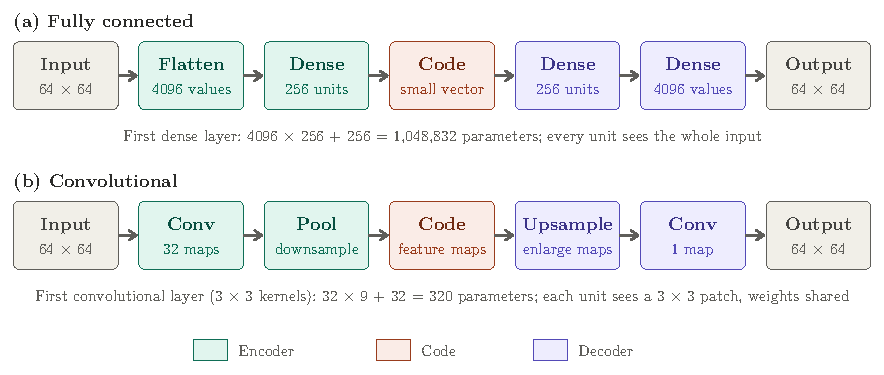
\includegraphics[width=\textwidth]{fig2-ae-architectures}
  \caption[Fully connected and convolutional autoencoders]{Fully connected (top) and convolutional (bottom) autoencoders for a $64 \times 64$ spectrogram. The dense encoder connects every input element to every unit; the convolutional encoder applies the same small kernels at every position. Parameter counts are for the first encoder layer. The layer sizes are illustrative; the architectures used in this study are given in Chapter~3. Based on \textcite[pp.~329--334]{goodfellow2016} and \textcite[p.~54]{masci2011}.}
  \label{fig:ae-architectures}
\end{figure}

These properties suit the spectrogram of an LTE carrier. The carrier appears as a band of raised power over contiguous frequency bins that persists in time, and where it falls within the window depends on the tuning (\cref{fig:obs-window}). A convolutional layer can detect the same local pattern, such as the edge of a carrier, wherever it occurs, whereas a dense layer must learn it separately at every position. This is the argument for the convolutional autoencoder as the primary model in this study. It is an argument, not a result. The empirical evidence on the two architectures is mixed. With the percentile score of \textcite{tian2022}, a fully connected variational autoencoder achieved a higher area under the curve than a convolutional one for Gaussian minimum-shift keying (GMSK) and chirp anomalies and a lower one for quadrature phase-shift keying (QPSK) and 16-point quadrature amplitude modulation (16QAM) anomalies (p.~8). \Textcite{xu2021} found the convolutional variant better by 0.016 in area under the curve, and better at low false-positive rates (p.~5). \Textcite{baset2023} found a shallow convolutional autoencoder sufficient for aviation signals; adding layers increased the prediction time without significantly improving detection. The architectural choice is therefore tested directly in this study, with a fully connected autoencoder trained on the same data (Chapter~4).

\subsection{Variational Autoencoders and Percentile Scores}
\label{sec:ae-vae}

A variational autoencoder (VAE) is a probabilistic version of the autoencoder. \Textcite{kingma2014} introduced a recognition model $q_{\phi}(\mathbf{z} \mid \mathbf{x})$, which approximates the intractable posterior distribution of a latent code $\mathbf{z}$ and acts as a probabilistic encoder, and a generative model $p_{\theta}(\mathbf{x} \mid \mathbf{z})$, which acts as a probabilistic decoder. Both are trained jointly by maximizing a lower bound on the likelihood of the data, which a reparameterization makes amenable to standard stochastic gradient methods; when the recognition model is a neural network, the result is the variational autoencoder (pp.~1--3).

For spectrum anomaly detection, \textcite{tian2022} trained VAEs on spectrograms of normal data and argued that the mean squared error pays equal attention to every part of the spectrum, which dilutes the effect of anomalies that are short or narrow in frequency (p.~2). They proposed a percentile (PER) score, which combines high percentiles of the pixel-level reconstruction errors in the background and signal regions of the spectrogram (p.~4). For QPSK anomalies, it raised the recall from \pct{80} to \pct{93} at a false-alarm rate of \pct{5} (p.~6). \Textcite{xu2021} proposed a related score that weights the reconstruction error towards low-amplitude, noise-like regions of the spectrogram, to which an anomaly raises the noise floor of the reconstruction (pp.~1, 3). Both scores show that how the reconstruction error is summarized can matter as much as the model. This study includes a VAE with the percentile score as a comparison with the MSE score (Chapter~3).

\subsection{Setting the Threshold}
\label{sec:ae-threshold}

An anomaly score becomes a detector only when a threshold is applied to it. A threshold can always be derived from the empirical distribution of the anomaly scores \parencite{ruff2021}. Studies differ in which scores they use and how. \Textcite{rajendran2019} applied an $n$-sigma rule to the reconstruction and discriminator losses, using their mean and standard deviation on the training data, with $n$ chosen empirically. \Textcite{baset2023} set the threshold at the 98th percentile of the reconstruction errors on the training data, which corresponds to a false-positive rate of \pct{2} on those data. \Textcite{torio2025} set it a chosen number of decibels above the activity of the least active channel, which they took as a noise-only reference (p.~9). For supervised detectors, \textcite{gao2019} noted that the lack of precise control of the false-alarm rate is a drawback of deep-learning detectors.

In this study every detector, learned or classical, is thresholded in the same way. The threshold is the empirical $(1 - \Pfa)$ quantile of the detector's scores on idle validation frames, which are held out from training, for a target $\Pfa$ of \pct{1} or \pct{5} (\cref{fig:threshold}; Chapter~3). This is the empirical counterpart of the Neyman--Pearson threshold of the energy detector (\cref{sec:detection-problem}). Because the validation frames are not used for training, the false-alarm rate they fix is not biased by any fitting of the model to its own training data, and all detectors are compared at the same operating points.

\begin{figure}[tbp]
  \centering
  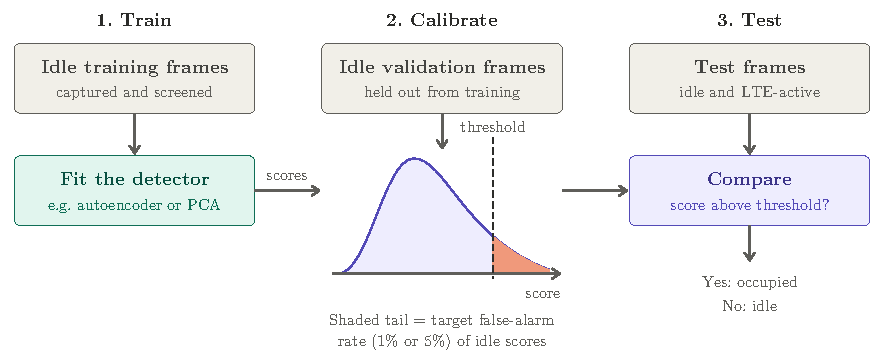
\includegraphics[width=\textwidth]{fig2-threshold-calibration}
  \caption[Threshold calibration on idle validation data]{Detection by reconstruction error with a threshold calibrated on idle data. The model is trained on idle frames only; its scores on held-out idle validation frames set the threshold at the $(1 - \Pfa)$ quantile; test frames whose score exceeds the threshold are declared occupied. The distribution sketch is schematic, not data. The same calibration is applied to every detector in this study.}
  \label{fig:threshold}
\end{figure}

\section{Related Work}
\label{sec:related}

This section reviews the studies closest to this thesis in two strands: learned spectrum anomaly detection (\cref{sec:related-anomaly}) and learned spectrum sensing compared with energy detection (\cref{sec:related-ed}). Low-cost monitoring systems were reviewed in \cref{sec:sdr}. \Cref{sec:related-practice} compares how the studies were evaluated, and \cref{tab:related-anomaly,tab:related-sensing} summarize them.

\subsection{Learned Spectrum Anomaly Detection}
\label{sec:related-anomaly}

Early work used prediction rather than reconstruction. \Textcite{oshea2016} trained recurrent predictors, chiefly a two-layer long short-term memory (LSTM) network, on raw IQ recordings made over the air with a USRP B200-mini in FM broadcast, cellular (GSM and LTE) and industrial, scientific and medical (ISM) bands (pp.~2--3). They injected five classes of synthetic anomalies into the recordings and detected them from the likelihood of the prediction error (pp.~2, 4). The neural predictors slightly outperformed a Kalman-filter predictor, with slightly larger improvements in the cellular bands, whose carriers have a more regular temporal structure (p.~6). \Textcite{tandiya2018} trained a deep predictive coding network on sequences of spectrogram images and spectral correlation images of normal network behaviour, generated in GNU Radio Companion, and reported detection of nearly \pct{100} at high SNR and \pct{90} at medium SNR for a false-alarm rate of 0.15 with the spectral correlation images.

Reconstruction models followed. \Textcite{rajendran2019} proposed SAIFE, an adversarial autoencoder that detects anomalies in PSD data and learns interpretable features in a semi-supervised way. They evaluated it on synthetic data, on sweeps recorded with a HackRF receiver in two Belgian cities and on data from Electrosense sensors, with synthetic anomalies injected into the real captures and the data split at random into equal training and test sets. \Textcite{rajendran2020} adapted SAIFE to crowdsourced sensing, using 56 days of spectrogram data from four Electrosense sensors built on low-cost RTL-SDR receivers sampling at \qty{2.4}{MS/s}. They trained on seven days and tested on the other 49, taken from non-adjacent periods. At constant false-alarm rates of \pct{5} and \pct{10}, SAIFE detected injected anomalies better than a one-class support vector machine, an isolation forest and the lightweight on-line detector of anomalies (LODA). The authors also observed that unsupervised threshold selection is difficult even with full knowledge of the anomalies.

Variational autoencoders on spectrograms were studied in the ISM band at \qty{2.4}{\giga\hertz}. \Textcite{xu2021} used a single capture of about \qty{41}{\minute}, split at random into training and test spectrograms, with chirp anomalies added digitally (p.~4). \Textcite{tian2022} recorded normal data in a laboratory and created anomalies by transmitting QPSK, 16QAM, GMSK and chirp signals from a second USRP, again with a random split of the normal data (p.~4). Neither study compared its detector with energy detection; Tian et al.\ compared their percentile score with MSE and mean absolute error scores and with classical outlier detectors (p.~6).

\Textcite{baset2023} built AviSense, a real-time monitor of aviation bands that combines a signal detector with autoencoder-based anomaly classification. Its signal detector is an energy detector refined by a spectral flatness measure, with a threshold recomputed at run time from blocks judged to be noise. When a threshold computed on one day was applied on another day, \pct{74.20} of the noise blocks were passed as signal, against \pct{32.79} to \pct{49.54} on the day of computation, which led the authors to conclude that a static threshold is impractical. Detected signals were then classified as normal or anomalous by shallow convolutional autoencoders trained on normal data only. Normal data were recorded at four locations with a USRP X310, a HackRF One or an RTL-SDR, and the test data deliberately varied the receiver, its gain, and the day, location and time of collection. AviSense ran on the central processing unit (CPU) of a laptop, and it is the only study in this group to report inference throughput.

\Textcite{torio2025} came closest to the present design. Treating the absence of transmissions as the normal state, they trained a one-dimensional convolutional autoencoder on synthetic Rayleigh-distributed noise sequences and applied it to day-long amplitude recordings from a regulator's monitoring station in the very high frequency (VHF) maritime and land mobile bands (pp.~4--5, 7). They compared it with a detector based on channel power, whose threshold was also set relative to the least active channel (p.~8). The two methods detected practically the same intervals. The autoencoder was more sensitive to low-power transmissions, whereas the power detector tolerated calibration imperfections better and needed no graphics processor (pp.~12, 14). They reported no probabilities of detection or false alarm.

\subsection{Learned Sensing versus Energy Detection}
\label{sec:related-ed}

A second strand trains supervised classifiers on labelled signal and noise examples and compares them with classical detectors. \Textcite{gao2019} trained DetectNet, a network of convolutional and LSTM layers, on single-carrier signals generated in simulation following the conventions of the RadioML2016.10a dataset. At a $\Pfa$ of \pct{5.92} and a $\Pd$ of \pct{90}, its SNR wall was \qty{3.15}{\decibel} lower than that of the energy detector for 16QAM signals, and for GFSK it was about \qty{5}{\decibel} lower across sample lengths. The energy detector's SNR wall, however, was calculated from a formula rather than measured on the same simulated frames. \Textcite{zheng2020} trained a residual convolutional network on power spectra and reported better detection than maximum--minimum eigenvalue and entropy detectors at false-alarm probabilities of 0.1, 0.01 and 0.001, particularly at low SNR. Their training data were simulated, and in their one over-the-air test the captured signals of the Aircraft Communications Addressing and Reporting System (ACARS) were combined with simulated noise. \Textcite{peng2020} trained a convolutional network on simulated raw IQ samples. It outperformed an energy detector and approached the optimal detector when tested on data like its training data, but its performance degraded significantly when the signal or channel changed, and unsupervised domain adaptation still left it worse than the energy detector. Fine-tuning with a few hundred labelled examples from the new domain restored its advantage.

Two studies point the other way or qualify the comparison. \Textcite{grosu2021}, using simulated OFDM signals over additive white Gaussian noise (AWGN), flat-fading and frequency-selective channels, found that an energy detector with a threshold set adaptively from the noise variance and a target false-alarm rate outperformed their neural network on average, especially at low SNR. A network trained on data concentrated in a narrow SNR range outperformed the energy detector only within that range (p.~11). \Textcite{saber2021} captured amplitude- and frequency-shift-keyed signals at \qty{433}{\mega\hertz} with an RTL-SDR and reported a $\Pd$ of 0.994 for their deep-learning classifier against 0.961 for energy detection. The detectors were compared at different false-alarm probabilities, however (0.0023 and 0.0120), the energy detector's threshold rule is described only by reference to earlier work, and the classifier they call a convolutional network is described in the text as fully connected. \Textcite{zeghdoud2023}, as reported in their abstract, found a detector that combines a convolutional neural network (CNN) with an LSTM network better than CNN, LSTM and energy detectors at low SNR in numerical simulation, and implemented real-time sensing on a USRP.

\subsection{Evaluation Practice}
\label{sec:related-practice}

\Cref{tab:related-anomaly,tab:related-sensing} show how differently these studies were evaluated, and the differences limit what can be concluded from them.

\begin{itemize}
  \item \emph{Data.} Five studies used simulated data only \parencite{tandiya2018,gao2019,zheng2020,peng2020,grosu2021}. Most studies with real captures injected synthetic anomalies into them \parencite{oshea2016,rajendran2019,rajendran2020,xu2021}; only \textcite{tian2022} and \textcite{baset2023} transmitted their anomalies over the air. No study evaluated the occupancy of an LTE downlink band; LTE appears only as one of the recorded bands of \textcite{oshea2016}.
  \item \emph{What is normal.} The anomaly detectors treat a band with its usual signals as normal. Only \textcite{torio2025} treated the absence of transmissions as normal, and their model was trained on synthetic noise. None of the studies trained a detector on captured idle spectrum.
  \item \emph{Energy-detector baselines.} Most anomaly-detection studies included no energy detector. Where one was included, its threshold was set adaptively from the noise variance \parencite{grosu2021}, relative to a reference channel \parencite{torio2025}, from an analytical formula \parencite{gao2019}, or in a way that is not described \parencite{saber2021,peng2020}. The finding of \textcite{baset2023} that a static energy threshold fails from one day to the next shows why the choice matters.
  \item \emph{Operating points.} Several studies reported results at fixed false-alarm rates \parencite{rajendran2020,tian2022,zheng2020,peng2020,gao2019,grosu2021}; others reported only receiver operating characteristic (ROC) curves, the area under them (AUC), or accuracy. Where thresholds were derived from data, they came from training-data statistics \parencite{rajendran2019,rajendran2020,baset2023}. None of the studies described calibrating a threshold on a separate held-out set of noise-only data.
  \item \emph{Splits and variability.} Random splits were common \parencite{rajendran2019,xu2021,tian2022}. Only \textcite{rajendran2020} separated training and test data by time, and \textcite{baset2023} varied receiver, gain, day and location in their test data. None of the thirteen studies reported confidence intervals.
  \item \emph{Computation.} Training on graphics processors was common \parencite{tandiya2018,rajendran2020,zheng2020}, and the autoencoder of \textcite{torio2025} required one. Only \textcite{baset2023} reported inference throughput on a laptop CPU, and none reported per-frame latency.
\end{itemize}

\begin{table}[tbp]
  \centering
  \footnotesize
  \setlength{\tabcolsep}{3pt}
  \caption[Related studies: learned spectrum anomaly detection]{Related studies of learned spectrum anomaly detection. ED: energy detector; FAR: false-alarm rate; ROC: receiver operating characteristic. The last row describes the design of this study, not its results.}
  \label{tab:related-anomaly}
  \begin{tabularx}{\textwidth}{@{} >{\raggedright\arraybackslash}p{2.1cm} >{\raggedright\arraybackslash}X >{\raggedright\arraybackslash}X >{\raggedright\arraybackslash}p{2.0cm} >{\raggedright\arraybackslash}p{1.9cm} >{\raggedright\arraybackslash}p{1.9cm} @{}}
    \toprule
    Study & Data and receiver & Task and model & ED baseline & Fixed FAR & Split \\
    \midrule
    \textcite{oshea2016} & Real recordings incl.\ GSM and LTE bands, USRP B200-mini; synthetic anomalies & Anomaly; LSTM predictor, normal-only & None (Kalman predictor) & Constant FAR, value not stated & Not stated \\
    \textcite{tandiya2018} & Simulated in GNU Radio & Anomaly; predictive coding on spectrogram and correlation images, normal-only & None & One point, 0.15 & Not stated \\
    \textcite{rajendran2019} & Synthetic; real HackRF and Electrosense PSD; injected anomalies & Anomaly; adversarial autoencoder & None & None (ROC) & Random \\
    \textcite{rajendran2020} & Real Electrosense RTL-SDR PSD, 56 days; injected anomalies & Anomaly; adversarial autoencoder, active learning & None & \pct{5}, \pct{10} & By time (7 / 49 days) \\
    \textcite{xu2021} & Real USRP capture, ISM band, one session; added chirps & Anomaly; convolutional and dense VAE & None & None (ROC) & Random \\
    \textcite{tian2022} & Real USRP laboratory capture, ISM band; transmitted anomalies & Anomaly; convolutional and dense VAE, percentile score & None & Recall at \pct{5} & Random \\
    \textcite{baset2023} & Real aviation bands, USRP X310, HackRF One, RTL-SDR; chamber and RadioML anomalies & Anomaly; shallow convolutional autoencoders & Front-end stage with adaptive threshold & Training-error percentile (\pct{2}) & Test varies receiver, gain, day, place \\
    \textcite{torio2025} & Real VHF amplitude recordings; training on synthetic noise & Transmission detection; 1-D convolutional autoencoder & Power detector, relative threshold & None & None (synthetic training) \\
    \addlinespace
    This study & Real LTE downlink captures, RTL-SDR Blog V4; captured idle data & Occupancy; convolutional and dense autoencoders, VAE, PCA, normal-only & Fixed and adaptive, same frames & \pct{1}, \pct{5} & By capture session \\
    \bottomrule
  \end{tabularx}
\end{table}

\begin{table}[tbp]
  \centering
  \footnotesize
  \setlength{\tabcolsep}{3pt}
  \caption[Related studies: learned spectrum sensing]{Related studies of learned spectrum sensing compared with classical detectors. ED: energy detector; FAR: false-alarm rate. Zeghdoud et al.\ (2023) is summarized from its abstract only. The last row describes the design of this study, not its results.}
  \label{tab:related-sensing}
  \begin{tabularx}{\textwidth}{@{} >{\raggedright\arraybackslash}p{2.1cm} >{\raggedright\arraybackslash}X >{\raggedright\arraybackslash}X >{\raggedright\arraybackslash}p{2.0cm} >{\raggedright\arraybackslash}p{1.9cm} >{\raggedright\arraybackslash}p{1.9cm} @{}}
    \toprule
    Study & Data and receiver & Task and model & ED baseline & Fixed FAR & Split \\
    \midrule
    \textcite{gao2019} & Simulated single-carrier signals & Sensing; supervised CNN--LSTM & Analytical SNR wall & \pct{5.92}; \pct{7} to \pct{9} & 3:1:1, method not stated \\
    \textcite{zheng2020} & Simulated; ACARS signals with simulated noise & Sensing; supervised residual CNN & None (eigenvalue, entropy) & 0.1, 0.01, 0.001 & Separate simulated sets \\
    \textcite{peng2020} & Simulated & Sensing; supervised CNN on IQ & Yes, threshold not described & 0.1 & Separate simulated sets \\
    \textcite{grosu2021} & Simulated OFDM & Sensing; supervised convolutional--LSTM & Adaptive threshold & 0.01 & Separate simulated sets \\
    \textcite{saber2021} & Real RTL-SDR laboratory captures, \qty{433}{\mega\hertz} & Sensing; supervised network & Yes, threshold not described & None (unequal FAR) & Not stated \\
    \textcite{zeghdoud2023} & Simulation; USRP demonstration & Sensing; supervised CNN--LSTM & Yes, in simulation & Not known & Not known \\
    \addlinespace
    This study & Real LTE downlink captures, RTL-SDR Blog V4; captured idle data & Occupancy; convolutional and dense autoencoders, VAE, PCA, normal-only & Fixed and adaptive, same frames & \pct{1}, \pct{5} & By capture session \\
    \bottomrule
  \end{tabularx}
\end{table}

\section{Research Gap}
\label{sec:gap}

Each element of the present design has precedents. Real captures from low-cost RTL-SDR receivers have been used for learned detection \parencite{rajendran2020,saber2021,baset2023}. Treating the absence of transmissions as the normal state has been tried \parencite{torio2025}, as has separating training and test data by time \parencite{rajendran2020}. Results have been reported at fixed false-alarm rates \parencite{zheng2020,grosu2021}, adaptive energy-detector thresholds have been used \parencite{grosu2021,baset2023}, and throughput on a laptop CPU has been measured \parencite{baset2023}. No reviewed study combines these elements, and none addresses the occupancy of an LTE downlink band.

The combination matters because the elements interact. The comparison between learned detectors and energy detection is mixed, and most of the evidence comes from simulation, from energy detectors whose thresholds were not tuned on the same data, or from comparisons at unequal false-alarm rates (\cref{sec:related-ed}). The one study that trained an autoencoder on noise used synthetic noise, measured no detection or false-alarm probabilities, and analysed one day of recordings \parencite{torio2025}. The one result on threshold stability across days concerns a static energy threshold \parencite{baset2023}; no study has asked whether a learned detector holds its calibrated false-alarm rate when the noise floor changes between sessions, although its input normalization and threshold are fixed once trained.

The gap is therefore the following. No study has evaluated, on real LTE downlink captures from a low-cost RTL-SDR, an autoencoder trained only on captured idle spectrum against carefully tuned classical baselines, including fixed-threshold and adaptive-threshold energy detectors, a PCA detector and a \syncsignal{} correlator. Such an evaluation must compare all detectors on identical frames, at false-alarm rates calibrated on held-out idle data, across capture sessions, with uncertainty estimates and with the computational cost of each detector measured on the hardware that would run it. The research questions of Chapter~1 address these points: RQ1 the comparison with energy detection at fixed $\Pfa$, RQ2 the value of non-linearity over PCA and the other baselines, RQ3 generalization across sessions and gain settings, RQ4 latency and throughput on the laptop's CPU, and RQ5 the effect of architecture and score.

\section{Summary}
\label{sec:lit-summary}

This chapter reviewed the background and related work for the study. An active LTE downlink carrier transmits reference signals in every subframe and synchronization signals every \qty{5}{\milli\second}, the latter only in its central \qty{1.08}{\mega\hertz}, while the RTL-SDR observes at most about \qty{2.56}{\mega\hertz} at a time. Occupancy detection is the sensing function on which cognitive radio and spectrum monitoring depend. Of the classical sensing methods, energy detection needs no knowledge of the signal, but its threshold depends on the noise power, and uncertainty in that power produces an SNR wall. Waveform-based detection with the LTE synchronization signals is more reliable but works only when the window covers the centre of the carrier. Low-cost SDRs make continuous monitoring affordable, at the price of hardware imperfections. Spectrograms preserve the time--frequency structure that energy detection discards. Autoencoders, linear PCA and variational autoencoders detect anomalies by reconstruction error, and convolutional architectures exploit the local, shift-invariant structure of spectrograms, although the evidence for them over dense models is mixed. The related work leaves open whether an autoencoder trained on captured idle spectrum outperforms tuned classical detectors on real LTE captures at fixed false-alarm rates and across sessions. Chapter~3 describes the method used to answer that question.

\chapter{Methodology}
\label{chap:method}

% Outline approved 2 November 2026 (notes/chapter3-outline.md). The design is
% fixed in notes/method-design.md; code/ implements it. Sources for every
% claim are listed in notes/chapter3-claims.md.
%
% Conventions while data collection is pending:
%  - \TBC{...}  (red, in brackets): a value set during data collection, e.g.
%    the band, the gain settings or the number of sessions captured.
%  - \Prov{...} (red): a provisional starting setting that may still be tuned
%    on training and validation data; frozen before the test data are scored.
%  - The chapter is written in the present tense as a description of the
%    design. Once the captures exist and the code has been run, it is to be
%    converted to the past tense with the values actually used.

\section{Introduction}
\label{sec:m-intro}

This chapter describes how the research questions of Chapter~1 are answered. It sets out the research design (\cref{sec:m-design}), the receiver, the band survey and the capture settings (\cref{sec:m-hardware}), the data classes and the capture sessions (\cref{sec:m-data}), the ground truth (\cref{sec:m-labels}) and the controlled-SNR test set (\cref{sec:m-injection}). It then describes the preprocessing (\cref{sec:m-preproc}), the session-level data splits (\cref{sec:m-splits}), the detectors (\cref{sec:m-detectors}) and the calibration of their thresholds (\cref{sec:m-thresholds}). The evaluation protocol, including the tests of the two hypotheses, is given in \cref{sec:m-eval}, the measurement of computational cost in \cref{sec:m-compute} and the real-time demonstration in \cref{sec:m-demo}. \Cref{sec:m-ethics} covers ethics, reproducibility and threats to validity, and \cref{sec:m-summary} summarizes the chapter.

\section{Research Design}
\label{sec:m-design}

The study is a comparative, quantitative evaluation of detectors on real captures. Every detector receives exactly the same frames of complex baseband samples recorded with the RTL-SDR Blog V4, and every detector is operated at the same false-alarm probabilities, calibrated in the same way on idle data that none of them has been trained on. Two kinds of test data are used. The over-the-air captures themselves are the uncontrolled conditions: their signal-to-noise ratio (SNR) and noise floor vary naturally between sessions, days and positions. A controlled-SNR test set, built by adding scaled LTE captures to idle captures in software, provides exact labels at set SNRs (\cref{sec:m-injection}). Data are split by capture session, never by frame, and every session is used as test data exactly once through session-level cross-validation (\cref{sec:m-splits}). Uncertainty is estimated over training seeds and, by bootstrap resampling, over sessions (\cref{sec:m-eval}).

\Cref{fig:m-overview} shows the pipeline from capture to evaluation, and \cref{tab:m-rq-map} links each research question and hypothesis to the data, detectors and analyses that address it.

\begin{figure}[tbp]
  \centering
  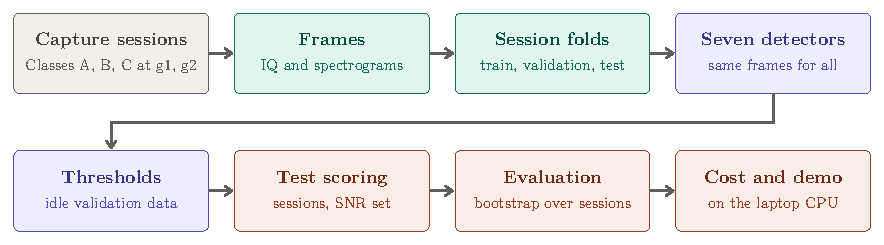
\includegraphics[width=\textwidth]{fig3-overview}
  \caption[Overview of the method]{Overview of the method. Captures from each session are framed and preprocessed once; all detectors score the same frames; thresholds are calibrated on idle validation sessions; test sessions and the controlled-SNR set are scored and evaluated with session-level uncertainty.}
  \label{fig:m-overview}
\end{figure}

\begin{table}[tbp]
  \centering
  \small
  \caption[Research questions and hypotheses mapped to the analyses]{Research questions and hypotheses of Chapter~1 mapped to the data, detectors and analyses of this chapter.}
  \label{tab:m-rq-map}
  \begin{tabularx}{\textwidth}{@{} >{\raggedright\arraybackslash}p{1.3cm} >{\raggedright\arraybackslash}X >{\raggedright\arraybackslash}X >{\raggedright\arraybackslash}X @{}}
    \toprule
    Item & Data & Detectors & Analysis \\
    \midrule
    RQ1 & Test sessions; controlled-SNR set & Convolutional autoencoder; fixed and adaptive energy detectors & $\Pd$ at $\Pfa = \pct{1}$ and \pct{5} by SNR (\cref{sec:m-eval}) \\
    RQ2 & As RQ1 & Convolutional autoencoder; PCA; \syncsignal{} correlator & As RQ1; paired differences with session bootstrap \\
    RQ3 & Pooled test folds; gain-$g_2$ captures & All & Realized $\Pfa$ and $\Pd$ across sessions, days, positions and the gain change \\
    RQ4 & Laptop CPU & All & Latency, throughput, real-time factor (\cref{sec:m-compute}) \\
    RQ5 & As RQ1 & Convolutional and fully connected autoencoders; VAE with MSE and percentile scores & As RQ1, with latent-size ablations \\
    H1 & Controlled-SNR set, SNR $\le \qty{-4}{\decibel}$ & Convolutional autoencoder versus adaptive energy detector & Bootstrap interval of $\Delta\Pd$ (\cref{sec:m-hypotheses}) \\
    H2 & Gain-$g_2$ captures of the test sessions & Convolutional autoencoder versus fixed energy detector (adaptive as reference) & Departures of realized $\Pfa$ and $\Pd$ from calibrated values (\cref{sec:m-hypotheses}) \\
    \bottomrule
  \end{tabularx}
\end{table}

\section{Hardware, Software and Band Selection}
\label{sec:m-hardware}

\subsection{Receiver and Host Computer}
\label{sec:m-receiver}

All captures are made with a single RTL-SDR Blog V4, whose specifications were summarized in \cref{tab:rtlsdr-v4}. It has an R828D tuner and an RTL2832U converter with 8-bit samples, tunes from \qty{500}{\kilo\hertz} to \qty{1.766}{\giga\hertz}, has a stable bandwidth of about \qty{2.56}{\mega\hertz} and a temperature-compensated reference oscillator with a tolerance of \qty{1}{ppm}, and provides a bias tee that can be switched in software \parencite{rtlsdrblog2024}. The receiver is connected over USB to the host laptop, a Dell Latitude 5490 with an Intel Core i5-8250U processor (four cores, eight threads), \qty{16}{\giga\byte} of memory and integrated graphics, running Ubuntu 26.04. All processing runs on the laptop's CPU except the training of the neural networks, which runs on a cloud graphics processing unit (GPU) provided by Google Colab (\cref{sec:m-training}). The trained detectors are scored, timed and demonstrated on the laptop, which is where a detector of this kind would be used. The software is written in Python and uses PyTorch \parencite{paszke2019} for the neural networks and scikit-learn \parencite{pedregosa2011} for PCA. \Cref{tab:m-hw-sw} lists the hardware and software, and \cref{app:install} describes how the receiver driver, the Python environment and the cell-search tool are installed.

\begin{table}[tbp]
  \centering
  \caption[Hardware and software]{Hardware and software used in the study. Library versions are those pinned in the project's lock file (\texttt{code/uv.lock}).}
  \label{tab:m-hw-sw}
  \begin{tabularx}{\textwidth}{@{} l >{\raggedright\arraybackslash}X @{}}
    \toprule
    Item & Value \\
    \midrule
    Receiver & RTL-SDR Blog V4 (R828D, RTL2832U, 8 bits) \\
    Antenna & \TBC{model, recorded in the capture metadata} \\
    Host & Dell Latitude 5490, Intel Core i5-8250U, \qty{16}{\giga\byte} RAM \\
    Operating system & Ubuntu 26.04 LTS \\
    Python & 3.12 \\
    PyTorch (CPU build) & 2.12.0 \\
    NumPy, SciPy & 2.4.5, 1.18.1 \\
    scikit-learn & 1.9.1 \\
    pyrtlsdr & 0.2.91 \\
    Receiver driver & \texttt{rtl-sdr-blog}, the manufacturer's fork of the RTL-SDR library, commit aed0ea1, built from source \parencite{rtlsdrblog2026} \\
    Survey tool & \texttt{rtl\_power} (from the RTL-SDR driver package) \\
    Cell-search tool & LTE-Cell-Scanner, program \texttt{CellSearch}, commit e7f71cb \parencite{peroulas2024} \\
    Training hardware & Google Colab GPU (\TBC{type and library versions, as recorded}) \\
    \bottomrule
  \end{tabularx}
\end{table}

\subsection{Band Survey}
\label{sec:m-survey}

Before any data are captured, the candidate bands are surveyed at the capture site. The survey's own measurements are not used to train or test any detector. Its role is to decide where and how the receiver is tuned for every capture that is used, and to document those decisions. Five settings of the study depend on it (\cref{tab:m-survey-role}).

\begin{table}[tbp]
  \centering
  \small
  \caption[Settings decided by the band survey]{Settings decided by the band survey.}
  \label{tab:m-survey-role}
  \begin{tabularx}{\textwidth}{@{} >{\raggedright\arraybackslash}p{3.0cm} >{\raggedright\arraybackslash}X >{\raggedright\arraybackslash}X @{}}
    \toprule
    Setting & Found from & Why it matters \\
    \midrule
    Band studied & Plateaus confirmed as carriers by the cell search, in every candidate range & An allocation does not mean that a carrier is on air at the site \\
    Carrier centre and bandwidth & Cell search on the chosen plateau & They place the C\textsubscript{centre} and C\textsubscript{offset} windows; C\textsubscript{offset} needs a carrier of at least \qty{10}{\mega\hertz} \\
    Idle (Class~B) window & A stretch of at least \qty{1.92}{\mega\hertz} with no signal above the noise floor, outside every carrier found & Its captures train the reconstruction models and give the idle frames of every evaluation \\
    Gains $g_1$ and $g_2$ & The strongest carrier, with trial captures & The strongest active capture must not clip the 8-bit converter \\
    Stability over the day & Surveys by day and at night & The carrier must be on air, and the idle window empty, at both session times \\
    \bottomrule
  \end{tabularx}
\end{table}

\emph{Sweeps.} Each candidate range is swept with \texttt{rtl\_power}, the spectrum-survey program of the RTL-SDR driver, at a fixed gain of \qty{40.2}{\decibel}, one of the tuner's steps; automatic gain is not used, for the same reason as in the captures (\cref{sec:m-capture}). The program steps the receiver across the range and records the power in frequency bins at most \qty{25}{\kilo\hertz} wide, averaged over \qty{10}{\second}. Each range is swept for \qty{10}{\minute}, which gives 60 readings for every bin. The readings are plotted as the mean power against frequency, together with the maximum over the readings, and as a waterfall of power against frequency and time. A narrow spike appears at the centre frequency of every tuning step of the sweep, in every reading; it is produced by the receiver, not by a signal, and is ignored. The sweep lasts minutes rather than seconds so that steady and intermittent signals can be told apart. A cell transmits reference signals in every downlink subframe \parencite[clause~6.10.1]{3gpp2026a}, so an active LTE carrier raises the power in every reading and appears as a flat plateau whose width matches one of the channel bandwidths of \cref{tab:lte-bandwidths}. An intermittent signal raises it in only some readings: it shows in the maximum but hardly in the mean, and as isolated marks in the waterfall. A single short sweep could not distinguish the two.

\emph{Cell search: why.} A plateau shows only that power is present in part of a range. It does not show which system transmits it, and its edges, blurred by the coarse bins of the sweep, give only estimates of where the signal begins and ends. A cell search settles both questions, and four parts of the method depend on it:
\begin{itemize}
  \item \emph{It confirms that a plateau is an LTE carrier.} The search detects the primary and secondary synchronization signals defined by the LTE standard \parencite[clause~6.11]{3gpp2026a} (\cref{sec:lte-sync}). A plateau counts as a carrier only if a cell is found at its centre, and the band studied is chosen among confirmed carriers only.
  \item \emph{It gives the carrier's exact centre and bandwidth.} The C\textsubscript{centre} window must be centred on the carrier, where the synchronization signals are, and the C\textsubscript{offset} window is placed at a distance from the centre that depends on the occupied width (\cref{sec:m-classes}). Both need the centre and bandwidth reported by the search, not estimates from the survey.
  \item \emph{It supports the ground truth.} A Class~C capture is labelled occupied only once a cell search has confirmed an active cell on the carrier (\cref{sec:m-labels}), and the cell identity shows whether the same cell is received in every session.
  \item \emph{It checks the idle window.} The centre and bandwidth of each carrier near the idle window show whether the window lies outside the band that the carrier occupies.
\end{itemize}

\emph{Cell search: how.} The search uses \texttt{CellSearch}, the cell-search program of LTE-Cell-Scanner, which was written for RTL2832-based receivers and is built here for the RTL-SDR \parencite{peroulas2024}. It tunes the receiver, at a fixed gain, to each frequency of a range in steps of \qty{100}{\kilo\hertz}, looks for the primary and secondary synchronization signals of a cell, and decodes the master information block (MIB) that the cell broadcasts. For each cell found it reports the physical-layer cell identity, the carrier frequency, the frequency offset, the received power and the bandwidth in resource blocks \parencite{peroulas2024}, which gives the carrier's channel bandwidth (\cref{tab:lte-bandwidths}). After each survey run, every plateau whose width is close to the occupied width of an LTE channel bandwidth is searched from \qty{0.5}{\mega\hertz} below to \qty{0.5}{\mega\hertz} above its centre, rounded to \qty{0.1}{\mega\hertz}, at a gain of \qty{40.2}{\decibel} and with two tries at each frequency. The program's output is kept with the survey records (\cref{app:survey}). At every session the search is repeated at the chosen carrier's frequency alone, before the captures, and the samples it captured are kept; the cell identity must be the one found in the survey.

\emph{Band.} The band cannot be fixed in advance. The candidate downlink ranges are those of \cref{tab:lte-bands} that the receiver can tune: \qtyrange{758}{803}{\mega\hertz} (Band~28), \qtyrange{790}{894}{\mega\hertz} (Bands~20 and~5 together) and \qtyrange{925}{960}{\mega\hertz} (Band~8). An allocation only permits operators to use a band; it does not show whether, or where in the band, a carrier is on air in Benin City. The band studied is therefore the one with the best confirmed carrier at the site: \TargetBand. Within it, the \qty{10}{\mega\hertz} carrier centred at \qty{773}{\mega\hertz} (cell identity 145) is used for the active captures; the reasons for this choice are given in \cref{app:survey}. The survey outputs are kept as evidence for this and the other choices (\cref{app:survey}).

\emph{Windows.} The survey also fixes where the receiver's \qty{1.92}{\mega\hertz} window is placed (\cref{fig:m-windows}). For active captures (Class~C, \cref{sec:m-data}), it is placed either on the carrier's centre, where it contains the synchronization signals, or inside the carrier away from its centre, where it does not (\cref{sec:lte-sync}). For idle captures (Class~B), it is placed on a stretch of the surveyed range at least \qty{1.92}{\mega\hertz} wide with no carrier, as close as possible to the carrier, so that the idle and active captures are made at nearly the same tuner frequency. With the chosen carrier, the C\textsubscript{centre} window is centred at \qty{773}{\mega\hertz}, the C\textsubscript{offset} window \qty{2.52}{\mega\hertz} above it, at \qty{775.52}{\mega\hertz}, and the idle window at \qty{765.37}{\mega\hertz}, in a stretch that was quiet by night and by day (\cref{app:survey}).

Of all the settings, the idle window has the largest consequences. The reconstruction models learn whatever their training frames contain as normal (\cref{sec:ae-anomaly}), and their training frames are the Class~B captures at $g_1$ (\cref{sec:m-training}). The same captures give the idle frames on which every detector's threshold is calibrated and its false alarms are counted (\cref{sec:m-thresholds,sec:m-eval}). A weak signal in the idle window that went unnoticed would therefore be learned as part of the noise floor, so that the networks could not detect it, and it would make the idle label of every frame in the window wrong, in training and in evaluation alike. Because frames are not screened individually (\cref{sec:m-labels}), the window has to be shown to be empty before any idle data are captured. In every frequency bin of the window, the mean power must stay within \qty{3}{\decibel} and the maximum over the readings within \qty{6}{\decibel} of the noise floor, so that narrow and intermittent signals are excluded as well as carriers; and the window must lie outside the band occupied by every carrier that the cell search finds near it.

\emph{Gains and times.} The survey also shows the strongest carrier, at which trial captures are made to choose the gains $g_1$ and $g_2$ (\cref{sec:m-capture}). It is made once by day and once at night, starting at 07:00 and 22:00 WAT, the times of the sessions (\cref{sec:m-sessions}). Labels are set for whole captures (\cref{sec:m-labels}), so they hold only if the carrier is on air, and the idle window empty, at both times; a carrier that is off at one of the times, or a transmitter that appears in the idle window at one of them, shows as a difference between the two surveys. The survey is made at P1 (\cref{sec:m-sessions}), before the first session; each of its two runs takes about half an hour for the sweeps, followed by the cell searches. Before the first session at P2, the chosen carrier is searched for there and the range containing it is swept once for \qty{10}{\minute}, to confirm that the carrier is received and the idle window is quiet at P2 as well.

\begin{figure}[tbp]
  \centering
  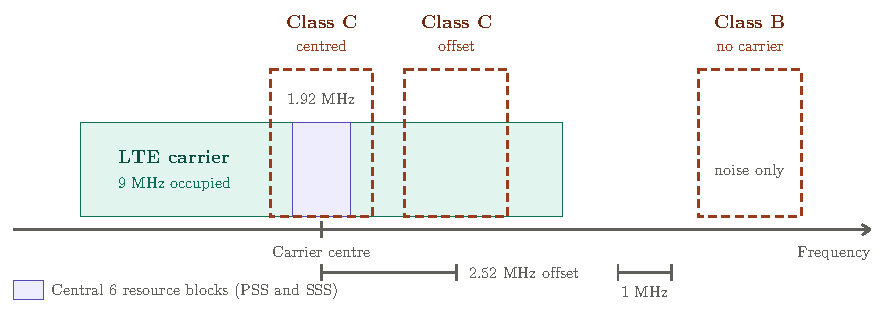
\includegraphics[width=\textwidth]{fig3-windows}
  \caption[Placement of the receiver windows]{Placement of the \qty{1.92}{\mega\hertz} receiver window for the three window types, shown for an example \qty{10}{\mega\hertz} carrier (\qty{9}{\mega\hertz} occupied), to scale in frequency. C\textsubscript{centre} is centred on the carrier and contains the PSS and SSS; C\textsubscript{offset} lies inside the carrier, clear of the central six resource blocks; B lies in a stretch with no carrier. Carrier widths from \textcite[Table~5.6-1]{3gpp2026b}; the central six resource blocks from \textcite[clause~6.11]{3gpp2026a}.}
  \label{fig:m-windows}
\end{figure}

\subsection{Capture Configuration}
\label{sec:m-capture}

\emph{Sample rate.} The receiver samples at $f_s = \qty{1.92}{MS/s}$. LTE timing is defined in units of $T_s = 1/(15000 \times 2048)$~s \parencite[clause~4]{3gpp2026a}, so $1/T_s = \qty{30.72}{\mega\hertz}$ and $f_s$ is exactly one sixteenth of it. At this rate the useful part of an OFDM symbol, $2048\,T_s$, is 128 samples, and the normal cyclic prefix of $160\,T_s$ or $144\,T_s$ is 10 or 9 samples \parencite[clause~6.12, Table~6.12-1]{3gpp2026a}. A 128-point fast Fourier transform (FFT) then has a bin spacing of \qty{15}{\kilo\hertz}, equal to the LTE subcarrier spacing \parencite[Table~6.2.3-1]{3gpp2026a}, and the PSS can be correlated against templates generated directly at the sample rate (\cref{sec:m-pss}). The observed window, \qty{1.92}{\mega\hertz} wide, is within the receiver's stable bandwidth of about \qty{2.56}{\mega\hertz} \parencite{rtlsdrblog2024} and contains the central \qty{1.08}{\mega\hertz} of a carrier when centred on it.

\emph{Gain.} Automatic gain control is never used, because it would change the noise floor during a capture. Two fixed gain settings are used: $g_1$, the primary setting, and $g_2$, used only for the gain-change test of \cref{sec:m-robustness}. For every capture the fraction of in-phase or quadrature samples at the extremes of the 8-bit range is recorded, and captures with more than \Prov{\pct{0.1}} clipped samples are flagged. The gains were chosen with trial captures on the chosen carrier after the survey (\cref{app:gains}). $g_1$ is the highest tuner gain step at which captures centred on the carrier stay below this limit even during traffic peaks, in which the carrier's power was seen to rise by several decibels; $g_2$ is the step \qty{10}{\decibel} lower. This gave $g_1 = \qty{29.7}{\decibel}$ and $g_2 = \qty{19.7}{\decibel}$. At these gains the idle level is set mainly by the receiver's own noise: lowering the gain from $g_1$ to $g_2$ lowered the idle level by about \qty{2}{\decibel}, while the carrier's level fell by about \qty{8}{\decibel} (\cref{app:gains}).

\emph{Other settings.} The bias tee is off for every capture: it must be off with the \qty{50}{\ohm} terminator of Class~A, and the antenna is passive. No frequency correction is applied (\qty{0}{ppm}), since the reference oscillator's tolerance is \qty{1}{ppm} \parencite{rtlsdrblog2024}; the value is recorded. Recording begins after the first \num{131072} samples (\qty{68}{\milli\second}) of the stream have been discarded. Each capture then lasts \Prov{\qty{30}{\second}}, giving \num{57600000} complex samples, which are stored as interleaved 8-bit unsigned integers (about \qty{115}{\mega\byte} per capture) with a metadata file.

\subsection{Metadata}
\label{sec:m-metadata}

A metadata record is written with every capture (\cref{tab:m-metadata}). It identifies the session, the position and the data class, records every receiver setting, and stores the cell-search result and the version of the capture software, so that every frame used in the evaluation can be traced to the conditions under which it was recorded.

\begin{table}[tbp]
  \centering
  \small
  \caption[Metadata recorded with each capture]{Metadata recorded with each capture.}
  \label{tab:m-metadata}
  \begin{tabularx}{\textwidth}{@{} >{\raggedright\arraybackslash}p{3.4cm} >{\raggedright\arraybackslash}X @{}}
    \toprule
    Group & Fields \\
    \midrule
    Identity & Capture, session and position identifiers; data class (A, B, C\textsubscript{centre}, C\textsubscript{offset}); start and end time (UTC) \\
    Receiver & Model and serial string; antenna; centre frequency; sample rate; gain; frequency correction; bias-tee state \\
    Measurements & Number of samples; clipping fraction; mean power; temperature, if available \\
    Ground truth & Cell-search tool and result (cell identity, carrier centre, bandwidth if known); operator notes \\
    Provenance & Version of the capture software (Git commit) \\
    \bottomrule
  \end{tabularx}
\end{table}

\section{Data Collection}
\label{sec:m-data}

\subsection{Data Classes}
\label{sec:m-classes}

Data are captured in three classes, the third in two window placements (\cref{fig:m-setup}).
\begin{itemize}
  \item \emph{Class A, receiver noise.} The antenna input is terminated with a matched \qty{50}{\ohm} load, so the capture contains only the receiver's own noise. Class~A is used to track the receiver noise floor across sessions and gain settings, and as a check of false alarms caused by the receiver alone. It is not used to train any detector.
  \item \emph{Class B, idle spectrum.} The antenna is connected and the window is placed where there is no LTE carrier (\cref{sec:m-survey}). Class~B contains the receiver noise together with whatever the environment contributes, and it is the normal class from which the reconstruction models learn and on which all thresholds are calibrated.
  \item \emph{Class C, LTE active.} The antenna is connected and the window lies on an active LTE carrier, either centred on it (C\textsubscript{centre}) or offset inside it (C\textsubscript{offset}). The offset places the window midway between the edge of the central six resource blocks, at \qty{\pm 0.54}{\mega\hertz}, and the edge of the occupied band: $f_\mathrm{off} = (\qty{0.54}{\mega\hertz} + W_\mathrm{occ}/2)/2$, where $W_\mathrm{occ}$ is the occupied width of \cref{tab:lte-bandwidths}. A window of \qty{1.92}{\mega\hertz} fits there only if the channel bandwidth is at least \qty{10}{\mega\hertz}; for a \qty{10}{\mega\hertz} carrier, $f_\mathrm{off} = \qty{2.52}{\mega\hertz}$. If the chosen carrier is narrower, C\textsubscript{offset} is not captured.
\end{itemize}

\begin{figure}[tbp]
  \centering
  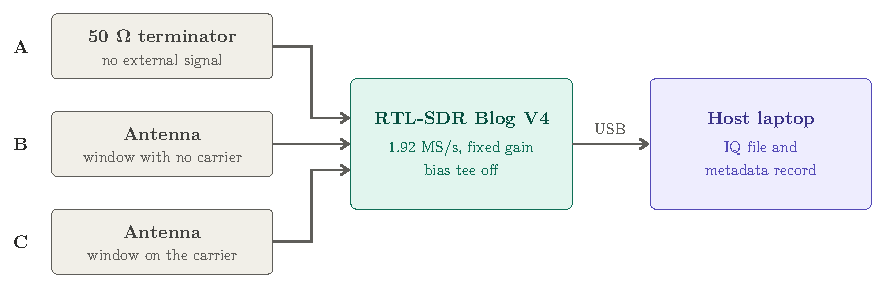
\includegraphics[width=\textwidth]{fig3-setup}
  \caption[Capture set-up for the data classes]{Capture set-up for the data classes. Class~A uses a \qty{50}{\ohm} terminator in place of the antenna; Classes~B and~C use the antenna and differ only in where the window is tuned (\cref{fig:m-windows}). The bias tee is off throughout.}
  \label{fig:m-setup}
\end{figure}

\subsection{Sessions}
\label{sec:m-sessions}

A session is one visit to one position, during which all classes are captured at both gain settings in a fixed order: A, B, C\textsubscript{centre} and C\textsubscript{offset}, each first at $g_1$ and then at $g_2$, so that the terminator is fitted and removed only once. That gives eight captures per session (\cref{tab:m-session-plan}). Sessions are the units of independence in the study: frames from the same session share the receiver's warm-up state, the antenna position and the local interference, so they are never split between training and test data. At least twelve sessions are planned, spread over at least four days and over two positions at the author's home in Benin City: the balcony of the sitting room (P1) and the balcony of a bedroom (P2). The two balconies face different directions, so the signals reach them from different directions and through different surroundings. At each position the antenna is mounted at a marked spot, at the same height and orientation in every session and at least \qty{30}{\centi\metre} from metal railings and bars, and the setup is photographed; the laptop stays indoors. Day sessions start at 07:00 and night sessions at 22:00 West Africa Time (WAT, UTC+1), the times of the survey. Each session is labelled day or night from the start time of its first capture; a session that starts more than two hours from both times is labelled off schedule and reported separately. The sessions actually captured are listed in \cref{app:sessions}.

\begin{table}[tbp]
  \centering
  \caption[Capture plan for one session]{Capture plan for one session. At \qty{1.92}{MS/s}, a \Prov{\qty{30}{\second}} capture yields \num{3515} frames of \num{16384} samples (\cref{sec:m-preproc}).}
  \label{tab:m-session-plan}
  \begin{tabular}{@{} c l l c c @{}}
    \toprule
    Order & Class & Window & Gain & Frames \\
    \midrule
    1, 2 & A & Antenna input terminated & $g_1$, $g_2$ & \num{3515} each \\
    3, 4 & B & No carrier & $g_1$, $g_2$ & \num{3515} each \\
    5, 6 & C\textsubscript{centre} & Carrier centre & $g_1$, $g_2$ & \num{3515} each \\
    7, 8 & C\textsubscript{offset} & Inside the carrier, off-centre & $g_1$, $g_2$ & \num{3515} each \\
    \bottomrule
  \end{tabular}
\end{table}

\section{Ground Truth}
\label{sec:m-labels}

Labels are set for whole captures, from the protocol and the cell search made at the time of capture. A Class~C capture is labelled occupied in every frame once the cell search has confirmed an active cell on the carrier. This is justified by the downlink structure: a cell transmits cell-specific reference signals in every downlink subframe \parencite[clause~6.10.1]{3gpp2026a}, so an active carrier occupies every frame of the window (\cref{sec:lte-sync}). A Class~B capture is labelled idle in every frame if the survey shows no signal in its window (\cref{sec:m-survey}) and no carrier found by the cell search occupies any part of it. Because the cell search finds a carrier at its centre frequency, the second condition is checked with the centre and bandwidth of each carrier near the window: the window must lie outside the band that the carrier occupies. Frames are not screened individually with any detector's statistic, because removing the idle frames that a detector finds suspicious would bias the evaluation in that detector's favour. Interference that appears in an idle window is therefore part of the idle class, as it would be in deployment.

The capture-level labels are checked in a second pass on a later day. The cell search is repeated where possible, and the mean spectrum and a sample of spectrograms of each capture are inspected for carriers. The agreement between the two passes is reported, and disagreements are resolved before evaluation. The labels are never used to train the reconstruction models; they only select the idle training data and score the detectors.

\section{Controlled-SNR Test Set}
\label{sec:m-injection}

The over-the-air captures provide realistic conditions but no control over SNR. The controlled-SNR test set provides that control with exact labels, by adding a scaled LTE capture to an independent idle capture (\cref{fig:m-injection}).

SNR is defined as the ratio of LTE signal power to noise power over the whole \qty{1.92}{\mega\hertz} window. For an idle frame $b$ from Class~B, the noise power $P_n(b)$ is its mean power, $\frac{1}{N}\sum \lvert b(n) \rvert^2$. For an active frame $c$ from Class~C, the signal power is estimated as
\begin{equation}
  P_s(c) = P(c) - \hat{P}_{n,C},
  \label{eq:m-ps}
\end{equation}
where $P(c)$ is the mean power of $c$ and $\hat{P}_{n,C}$ is the median noise power of the same session's Class~B frames at the same gain. A mixture with target SNR $\gamma$ is
\begin{equation}
  x = \alpha\, c + b, \qquad \alpha^2 = \frac{\gamma\, P_n(b)}{P_s(c)}.
  \label{eq:m-mix}
\end{equation}
Because $c$ carries its own noise, scaling it also adds $\alpha^2 \hat{P}_{n,C}$ of noise. The effective SNR of the mixture,
\begin{equation}
  \gamma_\mathrm{eff} = \frac{\alpha^2 P_s(c)}{P_n(b) + \alpha^2 \hat{P}_{n,C}},
  \label{eq:m-snr-eff}
\end{equation}
is therefore stored with each mixture and used for stratification. To keep $\gamma_\mathrm{eff}$ close to $\gamma$, only active frames whose natural SNR, $P_s(c)/\hat{P}_{n,C}$, exceeds the target by at least \Prov{\qty{10}{\decibel}} are used. The grid of targets runs from \qtyrange{-20}{10}{\decibel} in steps of \qty{2}{\decibel}, with \Prov{500} mixtures per level and session. Mixtures are built only within a test session, from frames recorded at different times, and separately for C\textsubscript{centre} and C\textsubscript{offset}.

\begin{figure}[tbp]
  \centering
  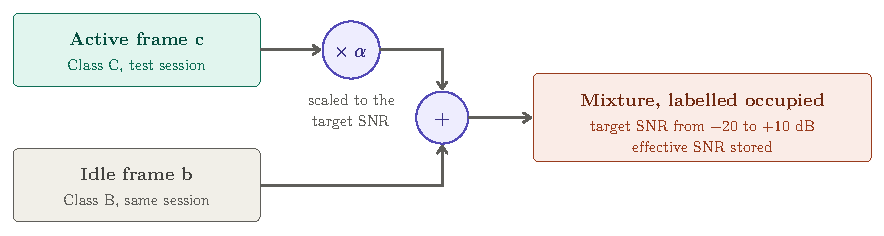
\includegraphics[width=\textwidth]{fig3-injection}
  \caption[Construction of the controlled-SNR test set]{Construction of the controlled-SNR test set. An active frame $c$ is scaled by $\alpha$ so that its estimated signal power reaches the target SNR $\gamma$ relative to the power of an idle frame $b$ from the same session, and the two are added. The effective SNR $\gamma_\mathrm{eff}$ accounts for the noise carried by $c$ (\cref{eq:m-snr-eff}).}
  \label{fig:m-injection}
\end{figure}

The mixtures are an approximation. The LTE frame already contains the receiver's noise and its 8-bit quantization, the noise added with it is environmental as well as thermal, and no fading is imposed beyond what the capture contains. The set is therefore used for controlled comparisons between detectors, while the over-the-air captures show performance under natural conditions. For hypothesis~H1, \enquote{low SNR} is defined as $\gamma \le \qty{-4}{\decibel}$ on this grid. These are the levels below the SNR wall of the energy detector for \qty{1}{\decibel} of noise uncertainty, \qty{-3.3}{\decibel} (\cref{eq:snr-wall}; \cite{tandra2008}), where an energy detector cannot be robust and a learned detector would have to show its advantage.

\section{Preprocessing}
\label{sec:m-preproc}

\emph{Frames.} Each capture is divided into non-overlapping frames of $N = \num{16384}$ complex samples, \qty{8.533}{\milli\second} at \qty{1.92}{MS/s} (\cref{fig:m-frame}). The PSS and SSS recur every \qty{5}{\milli\second} (\cref{sec:lte-sync}), so every frame of a C\textsubscript{centre} capture contains at least one complete pair. The mean of each frame's complex samples is subtracted to remove the receiver's direct-current offset \parencite{calvopalomino2015}. Every detector, classical or learned, receives the same DC-removed frames.

\emph{Spectrogram.} For the learned detectors and PCA, each frame is converted to a spectrogram (\cref{eq:stft-discrete}) with a 128-point FFT, a periodic Hann window of 128 samples and a hop of 128 samples, giving 128 frequency bins of \qty{15}{\kilo\hertz} by 128 time columns of \qty{66.7}{\micro\second}. One column is close to one OFDM symbol. The Hann window is chosen to reduce the spectral leakage from strong signals into neighbouring bins \parencite{harris1978}; the window length follows from the subcarrier spacing. Power is expressed in decibels, $S = 10 \log_{10}(\lvert X \rvert^2 + 10^{-12})$, and the bins are arranged so that frequency increases upwards when the spectrogram is drawn as an image.

\emph{Normalization.} The spectrograms are standardized with a single mean and standard deviation computed over all training frames of the current cross-validation fold, $x = (S - \mu)/s$. The same two numbers are applied unchanged to the validation and test frames, and no clipping or rescaling is applied to test data. The normalization therefore does not adapt to a changed noise floor; that is deliberate, because it is part of what H2 tests. \Cref{tab:m-preproc} lists the settings.

\begin{figure}[tbp]
  \centering
  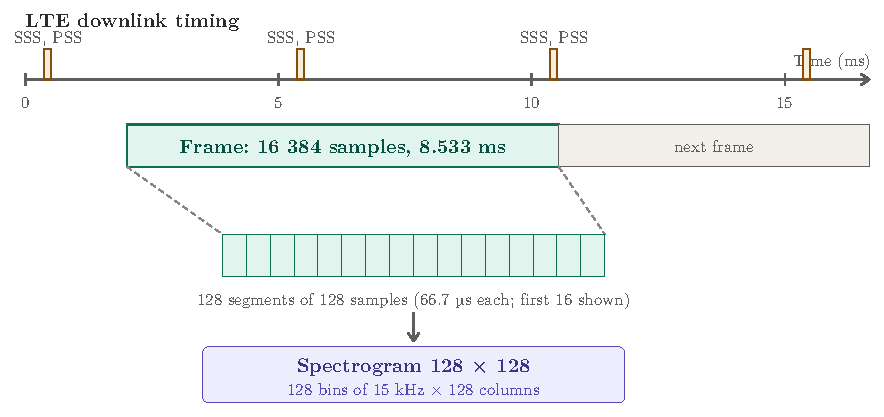
\includegraphics[width=\textwidth]{fig3-frame}
  \caption[Frame and spectrogram geometry]{Frame and spectrogram geometry. A frame of \num{16384} samples (\qty{8.533}{\milli\second}) is longer than the \qty{5}{\milli\second} period of the synchronization signals, so it always contains at least one PSS and SSS when the window covers the carrier centre. It is cut into 128 segments of 128 samples, each giving one spectrogram column of 128 bins of \qty{15}{\kilo\hertz}. Timing from \textcite[clauses~4.1, 6.11 and~6.12]{3gpp2026a}.}
  \label{fig:m-frame}
\end{figure}

\begin{table}[tbp]
  \centering
  \caption[Preprocessing settings]{Preprocessing settings.}
  \label{tab:m-preproc}
  \begin{tabularx}{\textwidth}{@{} l >{\raggedright\arraybackslash}X @{}}
    \toprule
    Setting & Value \\
    \midrule
    Sample rate & \qty{1.92}{MS/s} \\
    Frame length & \num{16384} samples (\qty{8.533}{\milli\second}), no overlap \\
    DC removal & Frame mean subtracted \\
    FFT size and window & 128 points, periodic Hann \\
    Hop & 128 samples (no overlap) \\
    Spectrogram size & $128 \times 128$ (frequency $\times$ time) \\
    Bin spacing; column duration & \qty{15}{\kilo\hertz}; \qty{66.7}{\micro\second} \\
    Scaling & $10\log_{10}$ power, then $(S-\mu)/s$ with training-fold $\mu$, $s$ \\
    \bottomrule
  \end{tabularx}
\end{table}

\section{Data Splits}
\label{sec:m-splits}

The data are split by session with four-fold cross-validation (\cref{fig:m-folds}). The sessions are divided into four groups of (at least) three. In each fold, one group is the test set, two sessions from the next group are the validation set, and the remaining sessions are the training set. Every session is therefore tested exactly once, always by models that have never seen it, and no frame from a test session is used for training, validation or normalization.

\begin{itemize}
  \item \emph{Training data:} Class~B frames at gain $g_1$ from the training sessions.
  \item \emph{Validation data:} Class~B frames at $g_1$ from the validation sessions. They are used for early stopping and for calibrating every threshold.
  \item \emph{Test data:} Class~B, C\textsubscript{centre} and C\textsubscript{offset} frames at $g_1$ from the test sessions, the controlled-SNR mixtures built from them, and, for the gain-change test, their captures at $g_2$.
\end{itemize}

With twelve sessions of \Prov{\qty{30}{\second}} captures, a fold has seven training sessions (about \num{24600} training frames), two validation sessions (about \num{7000} frames) and three test sessions.

\begin{figure}[tbp]
  \centering
  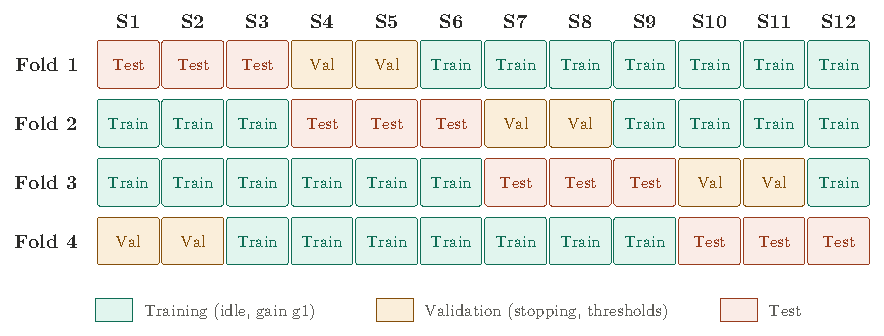
\includegraphics[width=\textwidth]{fig3-folds}
  \caption[Session-level cross-validation]{Session-level four-fold cross-validation with twelve sessions. In each fold, one group of three sessions is tested, two sessions of the next group are used for validation (early stopping and thresholds), and the rest are used for training. Every session is tested once.}
  \label{fig:m-folds}
\end{figure}

\section{Detectors}
\label{sec:m-detectors}

Seven detectors are compared (\cref{tab:m-detectors}). Four are learned from idle data: the three AI-based detectors, which are autoencoders (\cref{sec:ae}), and PCA, their linear counterpart. Of the other three, two are classical energy detectors and one exploits the known LTE synchronization signals. Each produces a score per frame, in which a larger value means that the frame is more likely to be occupied.

\begin{table}[tbp]
  \centering
  \small
  \caption[Detectors compared]{Detectors compared. All receive the same frames and are thresholded on the same idle validation data (\cref{sec:m-thresholds}).}
  \label{tab:m-detectors}
  \begin{tabularx}{\textwidth}{@{} >{\raggedright\arraybackslash}p{3.0cm} >{\raggedright\arraybackslash}X >{\raggedright\arraybackslash}X >{\raggedright\arraybackslash}X @{}}
    \toprule
    Detector & Input & Learned from & Score \\
    \midrule
    Convolutional autoencoder (primary) & Spectrogram & Idle training frames & Reconstruction MSE \\
    Fully connected autoencoder & Flattened spectrogram & Idle training frames & Reconstruction MSE \\
    Convolutional VAE & Spectrogram & Idle training frames & MSE; percentile score \parencite{tian2022} \\
    PCA & Flattened spectrogram & Idle training frames & Reconstruction MSE \\
    Fixed-threshold energy detector & DC-removed frame & Nothing (threshold only) & Average power $T$ \\
    Adaptive-threshold energy detector & DC-removed frame & Running noise estimate & $T$ divided by the noise estimate \\
    Synchronization\babelhyphen{hard}signal correlator & DC-removed frame & Nothing (threshold only) & Peak normalized correlation with the PSS \\
    \bottomrule
  \end{tabularx}
\end{table}

\subsection{Convolutional Autoencoder}
\label{sec:m-convae}

The primary detector is a convolutional autoencoder that takes the $128 \times 128$ spectrogram as a one-channel image (\cref{fig:m-convae}). Its encoder has three stages, each a $3 \times 3$ convolution followed by batch normalization and a rectified linear unit, with $2 \times 2$ max-pooling between stages and after the last. The stages have 16, 32 and 64 channels, as in the author's original model. A $1 \times 1$ convolution then reduces the 64 channels to \Prov{8}, so the code has \Prov{$8 \times 16 \times 16 = 2048$} values, an eighth of the input. The autoencoder is therefore undercomplete and must capture the most salient structure of idle spectrograms \parencite{goodfellow2016}. The decoder first maps the code back to 64 channels with a $1 \times 1$ convolution, then mirrors the encoder with bilinear $2 \times$ upsampling and $3 \times 3$ convolutions, and its output layer is linear. The network has \Prov{\num{47849}} trainable parameters. The anomaly score is the mean squared reconstruction error over the $D = \num{16384}$ elements of the spectrogram (\cref{sec:ae-pca}). The choice of a convolutional architecture follows the argument of \cref{sec:ae-architectures}; whether it is better than a fully connected one is tested, not assumed (RQ5).

\begin{figure}[tbp]
  \centering
  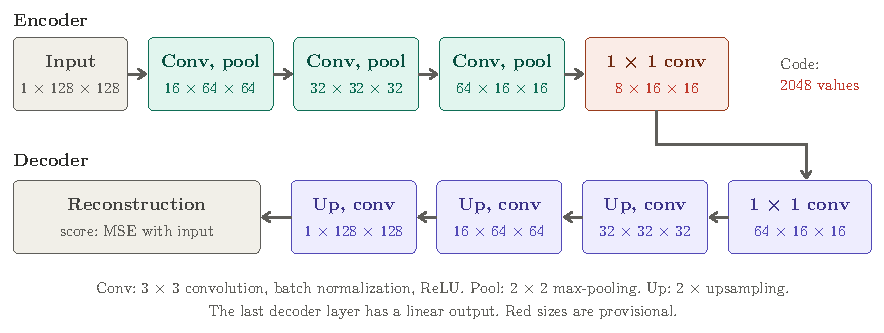
\includegraphics[width=\textwidth]{fig3-convae}
  \caption[Convolutional autoencoder]{The convolutional autoencoder, with tensor sizes (channels $\times$ frequency $\times$ time). Red sizes are provisional and may be tuned on validation data (latent channels 4, 8 or 16).}
  \label{fig:m-convae}
\end{figure}

\subsection{Fully Connected Autoencoder}
\label{sec:m-fcae}

The comparison model flattens the spectrogram to a vector of \num{16384} elements and passes it through dense layers of \Prov{256} and \Prov{128} units to the code, and back through \Prov{256} units to \num{16384} outputs, with rectified linear units between layers and a linear output. It has \Prov{\num{8471168}} trainable parameters, about 177 times as many as the convolutional autoencoder, almost all of them in its first and last layers. It is trained on the same data, with the same loss, optimizer and stopping rule as the convolutional model. Its code size is varied in an ablation (\Prov{32, 128 and 512}).

\subsection{Variational Autoencoder and Percentile Score}
\label{sec:m-vae}

The VAE uses the convolutional encoder and decoder of \cref{sec:m-convae}, with the encoder producing the mean and log-variance of a Gaussian code of \Prov{$8 \times 16 \times 16$} values \parencite{kingma2014}. It is trained to minimize the mean squared reconstruction error plus the Kullback--Leibler divergence of the code from a standard normal distribution, with weight \Prov{1}; at scoring time the code mean is decoded. Two scores are computed from the same reconstruction: the MSE, and the percentile score of \textcite{tian2022}, which combines high percentiles of the pixel-level errors in the background and signal regions of the spectrogram (\cref{sec:ae-vae}). The percentile score uses Tian et al.'s settings: a $3 \times 3$ kernel for the max- and min-pooling, a background weight of 2, a step threshold of 0.05 and the 90th and 99th percentiles (p.~4). Their description leaves two details open, which are fixed here as follows. The background mask is computed from a copy of the frame scaled to the range 0 to 1, and each percentile is taken over the pixels of its region only.

\subsection{PCA Detector}
\label{sec:m-pca}

The linear baseline projects the flattened, standardized spectrogram onto its leading principal components, computed from the training frames of the fold, and scores the frame by its mean squared reconstruction error \parencite{ruff2021}. The number of components is the smallest that explains at least \Prov{\pct{95}} of the training variance, capped at \Prov{256}. PCA is the linear counterpart of the autoencoder (\cref{sec:ae-pca}), so comparing them shows whether the non-linear model adds anything (RQ2).

\subsection{Energy Detectors}
\label{sec:m-ed}

Both energy detectors compute the average power of the DC-removed frame, $T = \frac{1}{N}\sum_{n=0}^{N-1} \lvert y(n) \rvert^2$ (\cref{eq:ed-statistic}), over all \num{16384} samples. They differ only in how their thresholds follow the noise power, the weakness identified in \cref{sec:ed}.

\begin{itemize}
  \item \emph{Fixed threshold.} The threshold on $T$ is calibrated once on the idle validation frames (\cref{sec:m-thresholds}) and never changes. This is equivalent to freezing the noise estimate at its validation value. It is the comparator for H2.
  \item \emph{Adaptive threshold.} A running noise estimate $\hat{\sigma}^2$ is kept as the median of $T$ over the most recent \Prov{$M = 64$} frames declared idle (about \qty{0.55}{\second}), initialized to the median of the validation frames. A frame is declared occupied if $T/\hat{\sigma}^2 > \kappa$. This is the constant-false-alarm-rate principle of estimating the noise level and setting the threshold relative to it \parencite[p.~121]{yucek2009}. The constant $\kappa$ is calibrated by running the same procedure over the validation stream. Each test session is processed as a stream in capture order (B, then C\textsubscript{centre}, then C\textsubscript{offset}), so the estimate can adapt to a session's noise floor before the active captures begin. An estimate is updated only by frames declared idle, so a long run of occupied frames leaves it unchanged. Because the updates depend on the decisions, the procedure is run separately for each target $\Pfa$. Mixtures of the controlled-SNR set are scored against the estimate held just before their idle frame, and Class~A captures form a stream of their own.
\end{itemize}

Under the Gaussian model of \cref{sec:ed}, the fixed threshold for a target $\Pfa$ could also be computed from the chi-square distribution of $T$ (\cref{eq:ed-threshold}). The empirical calibration is used instead, so that the energy detectors are calibrated exactly like the learned detectors. The theoretical threshold is reported for comparison.

\subsection{Synchronization-Signal Correlator}
\label{sec:m-pss}

The waveform-based detector (\cref{sec:waveform}) correlates each frame with the three possible PSS. For each root index $u \in \{25, 29, 34\}$ \parencite[Table~6.11.1.1-1]{3gpp2026a}, the length-62 Zadoff--Chu sequence $d_u(n)$ \parencite[clause~6.11.1.1]{3gpp2026a} is mapped to the subcarriers on either side of the unused DC subcarrier, $n = 0, \dots, 30$ to subcarriers $-31$ to $-1$ and $n = 31, \dots, 61$ to $+1$ to $+31$ \parencite[clause~6.11.1.2]{3gpp2026a}. A 128-point inverse FFT then gives the template $p_u(m)$, $m = 0, \dots, 127$, at the sample rate of the receiver. The score is the largest normalized correlation over the three templates and all lags $k$ at which the template lies wholly inside the frame:
\begin{equation}
  \Lambda_{\mathrm{PSS}} = \max_{u,\,k} \frac{\left\lvert \sum_{m} y(k+m)\, p_u^{*}(m) \right\rvert^2}{\sum_{m} \lvert y(k+m) \rvert^2 \, \sum_{m} \lvert p_u(m) \rvert^2},
  \label{eq:m-pss}
\end{equation}
which lies between 0 and 1 and does not depend on the receiver gain. With a frequency tolerance of \qty{1}{ppm} \parencite{rtlsdrblog2024}, the frequency error at the candidate bands is below about \qty{1}{\kilo\hertz}, a small fraction of the \qty{15}{\kilo\hertz} subcarrier spacing, so no frequency search is made. The correlator can only detect a carrier whose centre lies in the window: it is expected to work on C\textsubscript{centre} frames and to fail on C\textsubscript{offset} frames, and both results are reported. It tests only for the presence of the known sequences and decodes nothing.

\subsection{Training}
\label{sec:m-training}

The neural networks are trained with the Adam optimizer \parencite{kingma2015} (\cref{tab:m-training}). Training stops when the loss on the idle validation frames has not improved for \Prov{15} epochs, and the weights with the lowest validation loss are kept. Each model is trained with five seeds (0 to 4) in every fold, so that the variability due to initialization and batch order can be reported. Ablations of the code size use \Prov{three} seeds. The settings of \cref{tab:m-training} start from the author's original configuration, and any change made during development is based on training and validation data only.

Training runs on a GPU in Google Colab, a hosted notebook service, because training every network, fold and seed on the laptop's CPU would take weeks. The PCA detector needs no GPU and is fitted on the laptop. Only the data that training needs leave the laptop: the preprocessed Class~B spectrograms at $g_1$ of all sessions, the fold definitions, and the normalization statistics of each fold, computed on the laptop. Raw captures, active captures, captures at $g_2$, the controlled-SNR sets and all scores stay on the laptop. The idle spectrograms of every session are uploaded because each session is a training or validation session in some fold, but the training of a fold reads only that fold's training and validation sessions. A checksum of every uploaded file is verified before training. Each run saves a checkpoint at the end of every epoch and resumes from it after an interruption, because hosted sessions can be disconnected. The trained models are returned to the laptop. There they are checked against the local folds, settings, code and normalization statistics, and every expected run is checked for completeness and against its checksums, before the models are calibrated, evaluated and timed. To keep runs repeatable, the deterministic options of the GPU libraries are enabled. Results on a GPU are nevertheless not guaranteed to be bit-identical between runs, because some operations, such as the backward pass of bilinear upsampling, have no deterministic GPU implementation. The seeds still fix the initial weights and the order of the training batches. The GPU type and the library versions used are recorded with every model: \TBC{GPU and versions, from the training records}.

\begin{table}[tbp]
  \centering
  \caption[Training settings]{Training settings for the neural networks. Red values are provisional.}
  \label{tab:m-training}
  \begin{tabularx}{\textwidth}{@{} l >{\raggedright\arraybackslash}X @{}}
    \toprule
    Setting & Value \\
    \midrule
    Optimizer & Adam, learning rate \Prov{$10^{-3}$} (VAE \Prov{$10^{-4}$}), weight decay \Prov{$10^{-5}$} \\
    Batch size; maximum epochs & \Prov{64}; \Prov{100} \\
    Early stopping & Validation loss, patience \Prov{15} epochs \\
    Learning-rate schedule & Halved after \Prov{7} epochs without improvement \\
    Gradient clipping & Norm \Prov{1.0} \\
    Seeds & 0--4 (five per model and fold) \\
    Hardware & Google Colab GPU (\TBC{type}); laptop CPU (4 threads) for scoring \\
    \bottomrule
  \end{tabularx}
\end{table}

\section{Thresholds and Operating Points}
\label{sec:m-thresholds}

Every detector is operated at two target false-alarm probabilities, $\Pfa = 0.01$ and $0.05$. For each fold and detector, the threshold is the empirical $(1 - \Pfa)$ quantile of the detector's scores on the idle validation frames, taken so that at most a fraction $\Pfa$ of those scores exceeds it (\cref{fig:threshold}); for the adaptive energy detector it is $\kappa$, the quantile of $T/\hat{\sigma}^2$. A frame is declared occupied when its score exceeds the threshold. Thresholds are never set or adjusted on test data. The false-alarm rate realized on the test sessions' idle frames is reported next to the target, because a threshold calibrated on some sessions holds its rate on others only if the idle data do not change. That is the question behind RQ3 and H2.

\section{Evaluation Protocol}
\label{sec:m-eval}

\subsection{Metrics}
\label{sec:m-metrics}

For each detector, fold, seed and operating point, the predictions on the test frames give the metrics of \cref{tab:m-metrics}. Frames are counted as positives if occupied (Class~C or a mixture) and as negatives if idle (Class~B). Precision and the F1 score depend on the proportion of occupied frames in the test data, which is set by the capture plan rather than by the real occupancy of the band, so they are reported with that proportion. $\Pd$ and the realized $\Pfa$ do not depend on it. The receiver operating characteristic (ROC) curve and its area are computed from the scores without a threshold. Because each fold has its own models and score scale, the pooled curves use each score's position in its fold's idle validation distribution (its empirical quantile), so that scores from different folds are comparable.

\begin{table}[tbp]
  \centering
  \caption[Evaluation metrics]{Evaluation metrics. TP, FP, TN and FN are the counts of true positives, false positives, true negatives and false negatives, with occupied frames as positives.}
  \label{tab:m-metrics}
  \begin{tabularx}{\textwidth}{@{} l >{\raggedright\arraybackslash}X @{}}
    \toprule
    Metric & Definition \\
    \midrule
    Probability of detection, $\Pd$ (recall) & $\mathrm{TP}/(\mathrm{TP}+\mathrm{FN})$ \\
    Realized false-alarm rate, $\Pfa$ & $\mathrm{FP}/(\mathrm{FP}+\mathrm{TN})$ \\
    Precision & $\mathrm{TP}/(\mathrm{TP}+\mathrm{FP})$ \\
    F1 score & $2\,\mathrm{Precision}\cdot\Pd/(\mathrm{Precision}+\Pd)$ \\
    Confusion matrix & TP, FP, TN, FN at each operating point \\
    ROC curve and AUC & $\Pd$ against $\Pfa$ over all thresholds; area under it \\
    Precision--recall curve & Precision against recall over all thresholds \\
    \bottomrule
  \end{tabularx}
\end{table}

\subsection{SNR Stratification}
\label{sec:m-strata}

On the controlled-SNR set, $\Pd$ is reported at each level of the SNR grid, using the effective SNR of \cref{eq:m-snr-eff}. On the over-the-air C captures, the natural SNR of each frame, $P_s(c)/\hat{P}_{n,C}$ from \cref{eq:m-ps}, is estimated in the same way, and $\Pd$ is reported in bins of \Prov{\qty{2}{\decibel}}. Results for C\textsubscript{centre} and C\textsubscript{offset} are kept separate throughout.

\subsection{Uncertainty}
\label{sec:m-uncertainty}

Two sources of variability are reported. Variability due to training is the mean and standard deviation of each metric over the five seeds of each neural network; PCA and the classical detectors are deterministic and have no such variability. Variability due to the data is estimated with the bootstrap, which estimates the sampling distribution of a statistic from the observed data \parencite{efron1979}. Because frames within a session are not independent, the resampling units are sessions, not frames. The test predictions of the four folds are pooled, so that every session contributes once; \num{1000} bootstrap samples are drawn by resampling sessions with replacement, the metric, averaged over the five seeds, is recomputed on the frames of each sample, and the 2.5th and 97.5th percentiles give a \pct{95} interval. Differences between two detectors are bootstrapped in the same way, with both detectors evaluated on the same resampled sessions.

\subsection{Robustness}
\label{sec:m-robustness}

RQ3 is answered with three comparisons (\cref{tab:m-robustness}). Across sessions, the pooled cross-validation results already measure performance on sessions, days and positions that the models have not seen, and they are also broken down by session, by time of day (day or night sessions, \cref{sec:m-sessions}) and, where more than one position exists, by position. Across gain settings, the models and thresholds calibrated at $g_1$ are applied to the same test sessions' captures at $g_2$. The change of gain lowers the carrier's level by about \qty{8}{\decibel} but the idle level by only about \qty{2}{\decibel}, because the receiver's own noise dominates at these gains (\cref{sec:m-capture}); both changes are measured in every session. The receiver noise floor of each session and gain is tracked with the Class~A captures, so that changes of the idle data can be attributed to the receiver or to the environment.

\begin{table}[tbp]
  \centering
  \caption[Robustness comparisons]{Robustness comparisons for RQ3 and H2.}
  \label{tab:m-robustness}
  \begin{tabularx}{\textwidth}{@{} >{\raggedright\arraybackslash}p{3.0cm} >{\raggedright\arraybackslash}X >{\raggedright\arraybackslash}X @{}}
    \toprule
    Comparison & Training and calibration & Test \\
    \midrule
    Across sessions & Training and validation sessions of each fold, $g_1$ & Unseen test sessions, $g_1$ \\
    Across gain settings & As above, $g_1$ & The same test sessions, $g_2$ \\
    Across times and positions & As above & Pooled results broken down by time of day and position \\
    \bottomrule
  \end{tabularx}
\end{table}

\subsection{Hypothesis Tests}
\label{sec:m-hypotheses}

\emph{H1.} On the controlled-SNR set at gain $g_1$ and $\gamma \le \qty{-4}{\decibel}$, the difference
\begin{equation}
  \Delta\Pd = \Pd(\text{convolutional autoencoder}) - \Pd(\text{adaptive energy detector})
  \label{eq:m-h1}
\end{equation}
is computed at each operating point, pooled over the low-SNR levels. H1 is supported at an operating point if the \pct{95} bootstrap interval of $\Delta\Pd$ lies entirely above zero, and it is not supported otherwise. The primary test pools the mixtures built from C\textsubscript{centre} and C\textsubscript{offset} captures, and each source is also reported separately.

\emph{H2.} For the gain-$g_2$ test data, with thresholds calibrated at $g_1$, the departure of each detector from its calibrated behaviour is measured in two ways. The first is the absolute difference between the realized $\Pfa$ on the idle test frames and the target $\Pfa$. The second is the absolute difference between $\Pd$ at $g_2$ and at $g_1$ on the controlled-SNR set, with the mixtures of both sources pooled, averaged over the SNR levels that have mixtures at both gains. H2 is supported at an operating point if both departures of the convolutional autoencoder are smaller than those of the fixed-threshold energy detector, with \pct{95} bootstrap intervals of the paired differences entirely on that side. The adaptive energy detector is reported alongside as the reference for how much adaptation alone recovers.

\subsection{Failure Analysis}
\label{sec:m-failures}

For each detector a sample of false alarms and missed detections is inspected: their spectrograms, session, time of day, gain and estimated SNR. The aim is to relate errors to identifiable causes such as interference in the idle window, a changed noise floor or low SNR. Any cause found is reported with the results.

\section{Computational Cost}
\label{sec:m-compute}

\ref{rq:compute} asks whether the detectors can run in real time on the laptop. The question concerns the implementation as it would be used, so the scoring code of the neural networks is optimized (\cref{sec:m-optim}), and every detector is timed exactly as it is evaluated (\cref{sec:m-timing}).

\subsection{Optimization of Scoring}
\label{sec:m-optim}

Three changes reduce the work that the neural networks do for each frame. None of them may change a score beyond floating-point rounding, because the scores are what the evaluation compares, and the same scoring code is used in the evaluation, in the timing and in the demonstration.

\begin{itemize}
  \item \emph{Batch normalization folded into the convolutions.} When a trained network scores a frame, each batch-normalization layer multiplies every channel by one constant and adds another, both fixed by the statistics and parameters stored during training. The multiplication is therefore absorbed into the kernel of the convolution before the layer, and the addition into its bias, which removes one pass over every feature map of the convolutional networks.
  \item \emph{Channels-last memory order.} The feature maps of the convolutional networks are stored with the channels of each pixel next to each other, an alternative memory order that PyTorch supports for convolutions on the CPU, instead of one complete image per channel.
  \item \emph{Percentiles of the PER score.} The two percentiles of the PER score are computed with NumPy's percentile function instead of PyTorch's quantile function. Both interpolate linearly between order statistics and give identical values.
\end{itemize}

The fully connected autoencoder and the PCA detector contain neither convolutions nor batch normalization and are unchanged. The tests of the code (\cref{tab:app-tests}) check that the optimized networks reproduce the reconstructions of the trained networks to within $10^{-5}$ of the largest reconstructed value, and that the PER scores are identical. To measure the effect of the optimization, each neural network is also timed in its original form, as trained, with the original percentile computation. The two forms are timed on the same frames, alternating frame by frame, so that both see the same state of the laptop, and the ratio of their median latencies is reported in \cref{sec:r-compute}.

\subsection{Timing}
\label{sec:m-timing}

Latency and throughput are measured on the host laptop with the library versions of \cref{tab:m-hw-sw} and PyTorch limited to four threads, one per physical core of the processor. All timings are taken with the laptop on mains power and set to its Performance power profile, so that the processor runs at full speed and the timings are comparable; the timing program refuses any other known power state. Before any timing, every detector runs in turn for \qty{5}{\second}, because start-up effects of the program were found to slow the first detector timed for several seconds, longer than its own warm-up. After \num{50} warm-up frames, each detector then scores \num{1000} frames one at a time, and the time per frame is measured with Python's high-resolution performance counter. The median and the 95th percentile are reported separately for preprocessing (DC removal, spectrogram and standardization), for scoring, and end to end. Throughput is measured in frames per second with batches of 64 frames. The real-time factor is the processing time per frame divided by the frame duration, \qty{8.533}{\milli\second}; a value below one means the detector keeps up with the receiver. The CPU model, the thread count, the library versions and the power state are recorded with each measurement.

\section{Real-Time Demonstration}
\label{sec:m-demo}

The demonstration runs the complete chain live on the laptop (\cref{fig:m-demo}). Samples are read from the receiver at \qty{1.92}{MS/s} in blocks of one frame. Each frame is preprocessed and scored by the chosen detector with its calibrated threshold. The time, centre frequency, gain, score, decision and processing time of every frame are logged, and an optional live view shows the rolling spectrogram and the occupancy decisions; it is redrawn at most four times per second, and not while frames are waiting, so that it does not slow the detector. A short buffer of 32 frames (\qty{0.27}{\second}) separates reading from processing. If processing falls behind, the oldest frames are dropped and counted, so that the decisions stay current. Samples lost before they reach the program, for example by an overflow of the USB link, are estimated from the arrival times of the blocks and reported. Like the timings, the demonstration runs on mains power with the Performance profile. A short logged run on the chosen carrier (\cref{sec:m-survey}) illustrates occupancy over time in Chapter~4.

\begin{figure}[tbp]
  \centering
  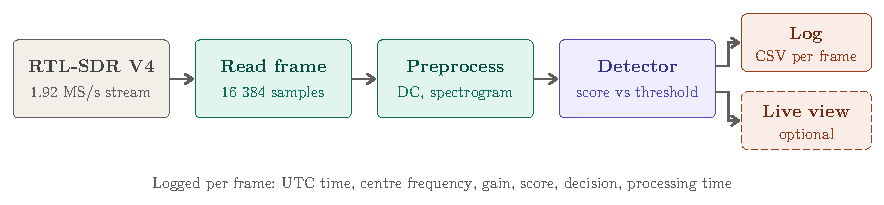
\includegraphics[width=\textwidth]{fig3-demo}
  \caption[Real-time demonstration]{Real-time demonstration. Frames are read from the receiver, preprocessed and scored as in the evaluation, and each decision is logged with its time and processing time.}
  \label{fig:m-demo}
\end{figure}

\section{Ethics, Reproducibility and Threats to Validity}
\label{sec:m-ethics}

\emph{Ethics.} Reception is passive: the study transmits nothing and measures only power and spectral structure. The \syncsignal{} correlator tests only for the presence of known sequences. The cell-search tool also decodes the MIB that each cell broadcasts, from which it reports only the carrier's bandwidth and two control-channel settings; only this mode of the tool is used, and no other system information, user data or other content is decoded or recorded.

\emph{Reproducibility.} Every result file records the configuration, the seeds, the version of the code and the library versions, and every trained model also records the device it was trained on. The code version is the Git commit together with a checksum of the source files; for the models trained on Colab, where Git is not available, it is the checksum, which must match that of the code on the laptop. The complete code is available at \url{https://github.com/jimroxodezi/masters-thesis}, and the modules that compute the reported results are listed in \cref{app:code}; the captures and labels are released if the supervisor approves.

\emph{Threats to validity.}
\begin{itemize}
  \item \emph{One receiver, one band, one city.} The results may not transfer to other receivers, bands or environments (Chapter~1). Two positions and two times of day widen the conditions but do not remove this limit. Both positions are at one home, so the transfer of a detector to another building, neighbourhood or set of base stations is not tested; the comparison between positions measures the effect of a change of direction and surroundings within one home.
  \item \emph{Labels.} Capture-level labels could be wrong if a carrier were missed in an idle window or a cell switched off during an active capture. The second labelling pass and the inspection of spectrograms reduce this risk.
  \item \emph{Idle data.} Interference in the idle windows is kept as part of the idle class. If it differs between sessions, it raises false alarms, which is a real effect rather than an artefact, but it complicates the comparison of sessions.
  \item \emph{Dynamic range.} The strong carrier limits the gain (\cref{app:gains}), so the idle data are dominated by the receiver's own noise and the environment contributes little to them. The results therefore describe detection against the noise of a low-cost receiver near a strong carrier, and the gain-change test shifts the idle level by only about \qty{2}{\decibel}.
  \item \emph{Controlled-SNR mixtures.} They approximate rather than reproduce weak signals (\cref{sec:m-injection}). The over-the-air captures complement them.
  \item \emph{Number of sessions.} With about twelve sessions the bootstrap intervals will be wide. Their width is reported rather than hidden.
  \item \emph{Tuning.} All settings are chosen on training and validation data. The test sessions are scored only after the configuration is frozen.
\end{itemize}

\section{Summary}
\label{sec:m-summary}

The method compares seven detectors on identical frames of real captures from an RTL-SDR Blog V4 sampling at \qty{1.92}{MS/s}, a rate tied to the LTE time unit. Data are captured in sessions, each with receiver noise, idle and active windows at two gain settings. Ground truth is set per capture and justified by the always-on reference signals of an active carrier. A controlled-SNR set with exact labels complements the natural captures. The learned detectors are trained only on idle frames. Every detector is calibrated on idle validation sessions at false-alarm probabilities of \pct{1} and \pct{5}, and evaluated on unseen sessions through session-level cross-validation, with uncertainty over seeds and sessions. Two hypotheses are tested with stated criteria, and the computational cost is measured on the laptop that would run the detector. Chapter~4 reports the results.

\chapter{Results and Discussion}
\label{chap:results}

% Outline approved 2 November 2026 (notes/chapter4-outline.md).
% SKELETON ONLY: no results exist yet (results/ is empty, no captures made).
% Every number, table and figure of this chapter is to be generated from
% results/ by the report step of code/ (decision D1); no result is typed by
% hand. Prose interpretation is written only after the evaluation has run.

\section{Introduction}
\label{sec:r-intro}

\TBC{Roadmap of the chapter, written once the results exist.}

\section{Band Survey and Chosen Band}
\label{sec:r-survey}

\TBC{Survey spectra by day and night, carriers found, cell-search results, the band chosen and the carrier bandwidth (which decides whether C\textsubscript{offset} captures were possible). Figure~4.1: survey spectrum with the windows marked. Full survey plots in \cref{app:survey}.}

\section{The Dataset}
\label{sec:r-data}

\TBC{Sessions captured, frames per class, clipping, agreement of the two labelling passes, noise floors by session and gain, and the natural-SNR distribution of the active captures. Table~4.1 (dataset summary); Figures~4.2 (example spectrograms of real frames) and~4.3 (noise floor by session and gain). Session list in \cref{app:sessions}.}

\section{Detection at Fixed False-Alarm Rates}
\label{sec:r-detection}

\TBC{RQ1, RQ2 and H1. Table~4.2: $\Pd$ on C\textsubscript{centre} and C\textsubscript{offset}, realized $\Pfa$ and AUC for the seven detectors at $\Pfa = \pct{1}$ and \pct{5}, with seed variability and session-bootstrap intervals. Figure~4.4: ROC curves. Figure~4.5: $\Pd$ against SNR on the controlled-SNR set. Table~4.3: the H1 test. The \syncsignal{} correlator on centred and offset windows; theoretical and empirical energy-detector thresholds.}

\section{Architecture and Score}
\label{sec:r-design}

\TBC{RQ5. Convolutional and fully connected autoencoders; VAE with the MSE and percentile scores; latent-size ablations; seed variability. Table~4.4 and Figure~4.6.}

\section{Generalization across Sessions and Gain}
\label{sec:r-general}

\TBC{RQ3 and H2. Per-session realized $\Pfa$ and $\Pd$ (Figure~4.7); breakdown by time of day and position; the gain-change test and the H2 verdict (Table~4.5, Figure~4.8); recovery by the adaptive energy detector; link to the Class~A noise floors.}

\section{Computational Cost and Real-Time Operation}
\label{sec:r-compute}

\TBC{RQ4. Latency (median and 95th percentile), throughput and real-time factor per detector on the laptop (Table~4.6); effect of the scoring optimization of \cref{sec:m-optim}: median latency of each neural network as trained and in its scoring form, and their ratio; occupancy over time from the demonstration log, with the numbers of dropped and missing blocks (Figure~4.9).}

\section{Failure Analysis}
\label{sec:r-failures}

\TBC{Examples of false alarms and missed detections with their likely causes (Figure~4.10).}

\section{Discussion}
\label{sec:r-discussion}

\TBC{Answers to RQ1--RQ5 and verdicts on H1 and H2, each tied to its table; comparison with the studies of Chapter~2 (\cref{sec:related}); practical implications, conceptually only; limitations and scope exclusions (no demodulation, downlink only, passive reception, one receiver, band and city; capture-level labels; the controlled-SNR approximation; the number of sessions).}

\section{Summary}
\label{sec:r-summary}

\TBC{Summary of the findings, written once the results exist.}

\chapter{Conclusion and Recommendations}
\label{chap:conclusion}

% Outline approved 2 November 2026 (notes/chapter5-outline.md), decisions D1
% and D2. Only the parts that do not depend on results are drafted; the rest
% are red \TBC notes. No finding is anticipated. Written in the present tense
% for now; convert to the past tense once the study is complete.

\section{Summary of the Study}
\label{sec:c-summary}

Occupancy detection is the step on which spectrum monitoring and dynamic spectrum access both depend: before a band's use can be measured or shared, it must be decided, observation by observation, whether a signal is present. The classical answer, energy detection, needs no knowledge of the signal but sets its threshold from the noise power, and errors in that power limit it at low SNR (Chapter~2). Learned detectors have been proposed as an alternative, but the evidence comparing them with energy detection is mixed and comes mostly from simulation, from baselines whose thresholds were not tuned on the same data, or from comparisons at unequal false-alarm rates.

This thesis examines whether AI-based detectors, autoencoders trained only on idle spectrum captured with a low-cost RTL-SDR receiver, detect the occupancy of an LTE downlink band better than carefully tuned classical detectors. The study captures its own data in Benin City: receiver noise, idle spectrum and active LTE carriers, in sessions spread over days, times, positions and two gain settings (Chapter~3). Seven detectors score identical frames. Four are learned from idle frames: three AI-based detectors, namely a convolutional, a fully connected and a variational autoencoder, and a PCA detector, their linear counterpart. The other three are classical: energy detectors with fixed and adaptive thresholds, and a correlator for the LTE synchronization signals. Every detector is calibrated on held-out idle sessions at false-alarm probabilities of \pct{1} and \pct{5} and evaluated on unseen sessions, with uncertainty estimated over training seeds and over sessions. A controlled-SNR set with exact labels complements the over-the-air captures, and the cost of each detector is measured on the laptop that would run it.

\section{Findings}
\label{sec:c-findings}

\TBC{One paragraph per research question and a verdict on each hypothesis, each pointing to its evidence in Chapter~4. Written only after the evaluation has run.}

\Cref{tab:c-answers} will collect the answers. Its evidence column is fixed by the design; its answers are filled in from the results of Chapter~4.

\begin{table}[tbp]
  \centering
  \small
  \caption[Answers to the research questions and hypotheses]{Answers to the research questions and hypotheses, with the evidence for each.}
  \label{tab:c-answers}
  \begin{tabularx}{\textwidth}{@{} >{\raggedright\arraybackslash}p{1.2cm} >{\raggedright\arraybackslash}X >{\raggedright\arraybackslash}p{3.6cm} @{}}
    \toprule
    Item & Answer & Evidence \\
    \midrule
    RQ1 & \TBC{after results} & \Cref{sec:r-detection} \\
    RQ2 & \TBC{after results} & \Cref{sec:r-detection} \\
    RQ3 & \TBC{after results} & \Cref{sec:r-general} \\
    RQ4 & \TBC{after results} & \Cref{sec:r-compute} \\
    RQ5 & \TBC{after results} & \Cref{sec:r-design} \\
    H1 & \TBC{supported or not supported, at each operating point} & \Cref{sec:r-detection} \\
    H2 & \TBC{supported or not supported} & \Cref{sec:r-general} \\
    \bottomrule
  \end{tabularx}
\end{table}

\section{Contributions}
\label{sec:c-contributions}

\TBC{The contributions of Section~1.6, revised to what the study actually delivered: the dataset (if released), the benchmark protocol, the comparison and the code. To be written together with the revision of Section~1.6.}

\section{Recommendations}
\label{sec:c-recommendations}

\subsection{For Practitioners}
\label{sec:c-rec-practice}

\TBC{Which detector to use for occupancy monitoring with a low-cost receiver, under which conditions, and how to calibrate it. These recommendations follow from the results and are written only after them.}

\subsection{For Researchers Evaluating Learned Detectors}
\label{sec:c-rec-research}

The review of Chapter~2 found that studies of learned spectrum detectors were evaluated in ways that make their conclusions hard to compare (\cref{sec:related-practice}). The design of this study answers those problems, and the same practices are recommended to others.

\begin{itemize}
  \item \emph{Split data by session, not by frame.} Frames recorded together share the receiver's state, the antenna position and the local interference, so a random split lets a model be tested on conditions it was trained on. Separating training and test data by time, as \textcite{rajendran2020} did, or by session, as here, tests what deployment requires.
  \item \emph{Calibrate thresholds on held-out idle data and report the realized false-alarm rate.} A threshold derived from training errors, or tuned on test data, does not show whether a detector holds its false-alarm rate on new data. The finding of \textcite{baset2023} that a static energy threshold failed from one day to the next shows why the realized rate should be reported, not assumed.
  \item \emph{Compare at the same operating point.} Detection probabilities are comparable only at equal false-alarm rates; comparisons at unequal rates, as in \textcite{saber2021}, cannot rank detectors.
  \item \emph{Give the classical baseline the same care.} An energy detector whose threshold is computed rather than calibrated on the same data, or whose noise estimate is never updated, is a weak baseline. Both a fixed and an adaptive variant, tuned on the same validation data as the learned detector, are needed to show what learning adds.
  \item \emph{Report uncertainty over the units of independence.} Intervals over sessions, and variability over training seeds, show how much a difference between detectors could be due to the particular data or initialization. None of the thirteen studies reviewed in Chapter~2 reported confidence intervals.
\end{itemize}

\TBC{Confirm or qualify these recommendations in the light of the results.}

\section{Limitations and Future Work}
\label{sec:c-future}

The limitations of the study are discussed with the results (\cref{sec:r-discussion}). Several directions for future work follow from the scope set in Chapter~1.

\begin{itemize}
  \item \emph{More receivers and cooperative sensing.} The study uses a single receiver at a time. Cooperation among sensors has been proposed to counter noise uncertainty, fading and shadowing \parencite{yucek2009}, and networks of low-cost sensors already exist \parencite{rajendran2018}. Whether a detector calibrated on one receiver transfers to another of the same model is an open question that this study does not test.
  \item \emph{Other bands and receivers.} The downlink of LTE Band~3 lies above the tuning range of the RTL-SDR (\cref{tab:lte-bands}). Repeating the study there, or in other bands, needs a receiver with a wider range.
  \item \emph{Other classical detectors.} The cyclostationary and eigenvalue-based detectors reviewed in \cref{sec:cyclo,sec:eigen} are not implemented here. The eigenvalue-based detectors need no estimate of the noise power \parencite{zeng2009}, which makes them natural further baselines for the noise-floor changes studied under H2.
  \item \emph{Other learned models.} Generative adversarial networks, diffusion models and other deep detectors are outside the scope of this study (Chapter~1) and could be compared under the same protocol.
  \item \emph{Longer-term monitoring.} The real-time demonstration logs occupancy for a short period. Logging over weeks would show daily and weekly patterns of use and test whether a detector's calibration holds over longer periods.
  \item \emph{Embedded deployment.} All processing runs on a laptop. Running the detectors on low-power embedded hardware, as monitoring networks do \parencite{calvopalomino2015,rajendran2018}, is excluded here and left for future work.
\end{itemize}

\TBC{Directions suggested by the results, for example the causes found in the failure analysis or, depending on the H2 result, adapting the autoencoder's normalization to the noise floor.}

\section{Closing Remarks}
\label{sec:c-closing}

\TBC{Written after the results.}


% ---------------------------------------------------------------------------
% References (APA 7)
% ---------------------------------------------------------------------------
\printbibliography[heading=bibintoc,title={References}]

% ---------------------------------------------------------------------------
% Appendices (A: band survey and capture sessions, filled after the fieldwork;
% B: code listings, read from code/ at compile time; C: software installation)
% ---------------------------------------------------------------------------
\appendix
% Make \cref print "Appendix B" rather than "Chapter B" for appendix chapters.
\crefalias{chapter}{appendix}
\chapter{Band Survey and Capture Sessions}
\label{app:a}

% Approved 2 November 2026 (Chapter 4 outline, decision D2). Filled after the
% band survey and the capture sessions; the session table is to be generated
% from the capture metadata by the report step of code/.

\section{Band Survey}
\label{app:survey}

The survey was made at P1, the sitting-room balcony (\cref{sec:m-sessions}), with the procedure of \cref{sec:m-survey}. The night run began at 22:10 WAT on 4 November 2026 (21:10 UTC) and the day run at 07:00 WAT on 5 November 2026 (06:00 UTC), with the antenna left in place between them. In each run the three candidate ranges were swept one after another, each for \qty{10}{\minute} at a gain of \qty{40.2}{\decibel}, giving 60 readings per frequency bin in bins of about \qty{21}{\kilo\hertz}. The noise floor of each range was the same in both runs to within \qty{0.1}{\decibel}. The cell searches followed each run, between 22:48 and 23:05 and between 07:32 and 07:49 WAT, each from \qty{0.5}{\mega\hertz} below to \qty{0.5}{\mega\hertz} above the plateau's centre, at the same gain and with two tries at each frequency. \Cref{fig:app-survey} shows the mean power in each range, \cref{tab:app-survey} the plateaus found and the result of the cell search on each, and \cref{tab:app-quiet} the quiet stretches that could hold the idle window.

\begin{figure}[tbp]
  \centering
  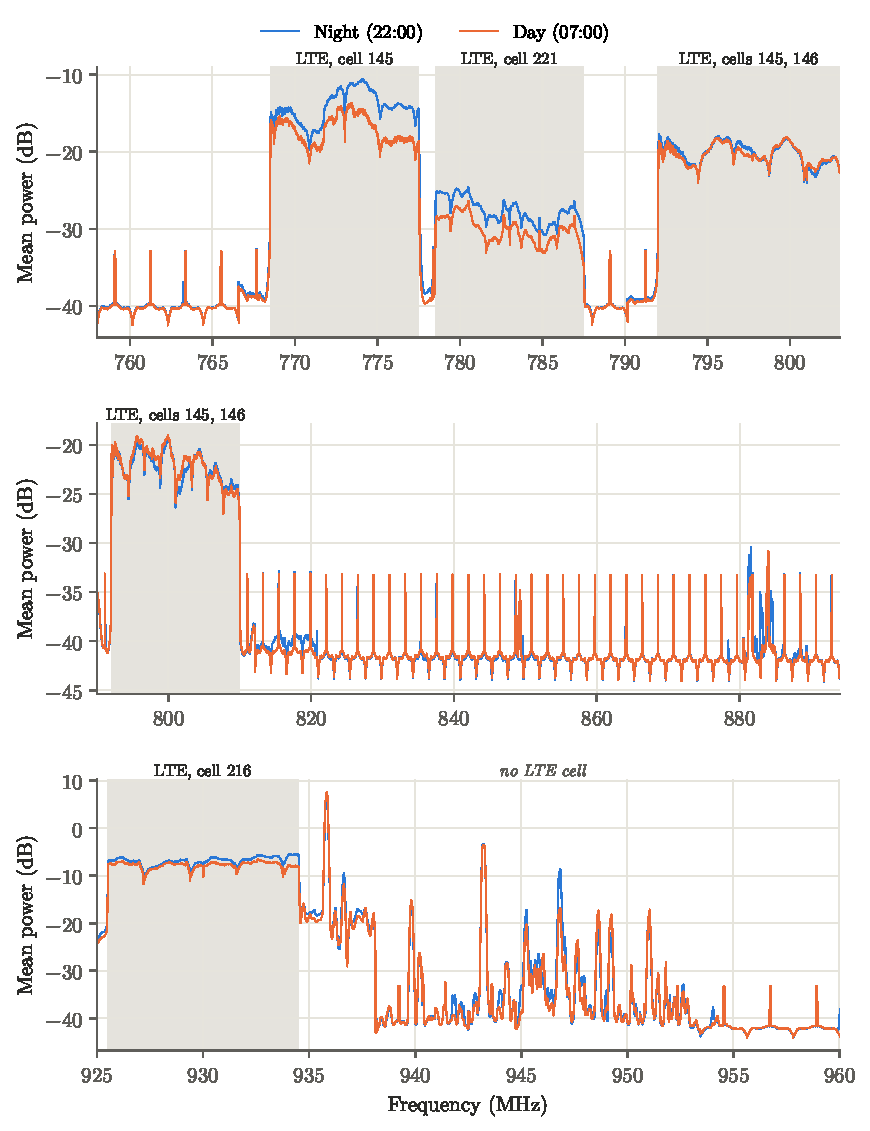
\includegraphics[width=\textwidth]{figA-survey}
  \caption[Band survey at P1]{Band survey at P1 by night and by day: mean power over the 60 readings of each candidate range, on the receiver's uncalibrated scale. Shaded: carriers confirmed by the cell search, drawn over their occupied width (number of resource blocks $\times$ \qty{0.18}{\mega\hertz}). The narrow spikes evenly spaced about \qty{2.2}{\mega\hertz} apart are produced by the receiver at the centre of each tuning step and are not signals.}
  \label{fig:app-survey}
\end{figure}

\begin{table}[tbp]
  \centering
  \small
  \caption[Band survey: plateaus and cell searches]{Band survey at P1: plateaus found in each candidate range and the result of the cell search on each, by night (N, 4 November 2026) and by day (D, 5 November 2026). Frequencies and widths in \unit{\mega\hertz}, from the night run; level in \unit{\decibel}: median mean power of the plateau above the noise floor of its range. The received power is as reported by the cell-search program, on its own relative scale.}
  \label{tab:app-survey}
  \begin{tabularx}{\textwidth}{@{} l l r l >{\raggedright\arraybackslash}X @{}}
    \toprule
    Range & Plateau & Width & Level N / D & Cell search (N and D) \\
    \midrule
    758--803 & 768.4--777.7 & 9.23 & 26.1 / 22.9 & LTE, FDD, cell 145, 50 resource blocks (\qty{10}{\mega\hertz}), centre \qty{773}{\mega\hertz}; \qty{-10.1}{} / \qty{-9.5}{\decibel} \\
     & 778.3--787.5 & 9.18 & 12.7 / 10.3 & LTE, FDD, cell 221, 50 resource blocks (\qty{10}{\mega\hertz}), centre \qty{783}{\mega\hertz}; \qty{-25.8}{} / \qty{-26.2}{\decibel} \\
     & 792.0--803.0 & 11.07 & 20.3 / 20.0 & Cut off at the end of the range; searched in the next range \\
    790--894 & 792.0--810.1 & 18.10 & 20.8 / 21.3 & LTE, FDD, cells 145 and 146, 100 resource blocks (\qty{20}{\mega\hertz}), centre \qty{801}{\mega\hertz}; \qty{-19.3}{} and \qty{-20.1}{} / \qty{-20.8}{} and \qty{-22.5}{\decibel} \\
    925--960 & 925.0--938.2 & 13.18 & 35.1 / 34.2 & A flat part, 925.5--934.5~MHz, followed by narrow peaks; searched at the centre of the flat part: LTE, FDD, cell 216, 50 resource blocks (\qty{10}{\mega\hertz}), centre \qty{930}{\mega\hertz}; \qty{-8.0}{} / \qty{-16.5}{\decibel} \\
     & 944.9--947.3 & 2.36 & 11.7 / 11.1 & No LTE cell found in either run (a cluster of narrow peaks, \qty{1.17}{\mega\hertz} wide by day) \\
    \bottomrule
  \end{tabularx}
\end{table}

Four LTE carriers were confirmed in both runs, with the same cell identities, and all with a channel bandwidth of at least \qty{10}{\mega\hertz}, so that C\textsubscript{offset} captures are possible on any of them (\cref{sec:m-classes}). Their levels changed by at most \qty{3.2}{\decibel} between night and day. Two cells, 145 and 146, were received on the same carrier at \qty{801}{\mega\hertz}; cell identity 145 was also found on the carrier at \qty{773}{\mega\hertz}. The crystal correction factors reported by the ten successful cell searches lay between 0.99999959 and 1.00000023, a receiver frequency error between \qty{-0.41}{ppm} and \qty{+0.23}{ppm}, within the \qty{1}{ppm} tolerance of the reference oscillator; this supports capturing without frequency correction (\cref{sec:m-capture}). Between 812 and \qty{821}{\mega\hertz} a weak signal was present by night but not by day, so that stretch is quiet only by day (\cref{tab:app-quiet}).

\begin{table}[tbp]
  \centering
  \small
  \caption[Band survey: quiet stretches]{Band survey at P1: quiet stretches at least \qty{1.92}{\mega\hertz} wide in which an idle window could be placed (\cref{sec:m-survey}), by night (N) and by day (D), the centre of the window suggested within each, and the largest mean and maximum power above the noise floor within that window.}
  \label{tab:app-quiet}
  \begin{tabular}{@{} l c l r r r @{}}
    \toprule
    Range (\unit{\mega\hertz}) & Run & Stretch (\unit{\mega\hertz}) & Centre (\unit{\mega\hertz}) & Mean (\unit{\decibel}) & Max.\ (\unit{\decibel}) \\
    \midrule
    758--803 & N & 758.0--763.2 & 760.6 & 0.8 & 1.5 \\
     & N & 763.2--766.6 & 764.9 & 0.8 & 1.4 \\
     & N & 787.5--791.9 & 789.7 & 1.7 & 2.7 \\
     & D & 758.0--766.6 & 762.3 & 0.8 & 1.4 \\
     & D & 787.5--791.9 & 789.7 & 1.4 & 3.1 \\
    790--894 & N & 820.8--834.3 & 827.6 & 1.8 & 2.7 \\
     & N & 834.4--849.6 & 842.0 & 1.9 & 3.4 \\
     & N & 849.6--864.0 & 856.8 & 1.8 & 2.5 \\
     & N & 864.0--878.4 & 871.2 & 1.7 & 2.4 \\
     & N & 889.5--894.0 & 891.8 & 1.6 & 2.5 \\
     & D & 812.2--849.0 & 830.6 & 1.9 & 3.3 \\
     & D & 849.4--864.0 & 856.7 & 1.8 & 3.0 \\
     & D & 864.0--880.5 & 872.3 & 1.6 & 2.6 \\
     & D & 885.2--894.0 & 889.6 & 1.9 & 5.3 \\
    925--960 & N & 954.3--960.0 & 957.1 & 0.6 & 1.1 \\
     & D & 952.9--960.0 & 956.5 & 0.7 & 1.3 \\
    \bottomrule
  \end{tabular}
\end{table}

\emph{Choice of band, carrier and idle window.} The band studied is \TargetBand, and the carrier used for the active captures is the \qty{10}{\mega\hertz} carrier centred at \qty{773}{\mega\hertz} (cell identity 145); the choice was confirmed by the author on 5 November 2026. This carrier was strong and steady, \qtyrange{22.9}{26.1}{\decibel} above the noise floor in the two runs; a single cell was received on it; and its bandwidth allows C\textsubscript{offset} captures. Most importantly, the stretch from 758.0 to \qty{766.6}{\mega\hertz} beside it was quiet in both runs, so that the idle window could be placed in the same band, close to the carrier and away from any narrow or intermittent signal. The idle window is centred at \qty{765.37}{\mega\hertz} (\qtyrange{764.41}{766.33}{\mega\hertz}), the window suggested nearest the carrier in both runs: within it, the mean power stayed within \qty{0.8}{\decibel} and the maximum within \qty{1.6}{\decibel} of the noise floor, and it lies about \qty{2.2}{\mega\hertz} below the band occupied by the carrier. The C\textsubscript{offset} window is placed above the carrier's centre, at \qty{775.52}{\mega\hertz}, in every session. The other confirmed carriers were less suitable. The carrier at \qty{783}{\mega\hertz} was \qtyrange{12.6}{13.4}{\decibel} weaker; the one at \qty{801}{\mega\hertz} carried two cells, and the stretch beside it, from 812 to \qty{821}{\mega\hertz}, was quiet only by day; and the one at \qty{930}{\mega\hertz} was strong enough to risk clipping, with narrow peaks between it and its nearest quiet stretch, about \qty{27}{\mega\hertz} away.

\section{Choice of the Gains}
\label{app:gains}

The gains $g_1$ and $g_2$ were chosen with trial captures on 5 November 2026, between 07:57 and 08:02 WAT, at P1 with the antenna as in the survey (\cref{sec:m-capture}). The captures were made with the study's capture program under the session identifier \texttt{trial}, and were then moved out of the data folder, to \texttt{data/trials/2026-11-05\_gain\_trials/}, so that they are never used as study data. The commands were, with \texttt{G} the tuner gain step of each capture:
\begin{lstlisting}[language=bash]
# carrier: 2 s captures at G = 40.2, 38.6, 37.2, 36.4, 33.8, 32.8, 29.7, 28.0, 25.4,
# 22.9 and 20.7 dB, then once more at 37.2 dB
uv run python -m occupancy capture --session trial --position P1 --class C_centre --gain-role g1 --gain G --freq 773M --duration 2 --notes "gain trial"
# idle window: 2 s captures at G = 29.7 and 19.7 dB
uv run python -m occupancy capture --session trial --position P1 --class B --gain-role g1 --gain G --freq 765.37M --duration 2 --notes "gain trial"
# carrier: one full-length (30 s) capture at 29.7 dB
uv run python -m occupancy capture --session trial --position P1 --class C_centre --gain-role g1 --gain 29.7 --freq 773M --duration 30 --notes "gain trial"
# idle window: 2 s captures at G = 22.9, 25.4, 29.7, 33.8, 36.4, 38.6, 40.2, 42.1, 44.5,
# 48.0 and 49.6 dB
uv run python -m occupancy capture --session trial --position P1 --class B --gain-role g1 --gain G --freq 765.37M --duration 2 --notes "gain trial: idle level vs gain"
# summary of all trial captures (Tables A.3 and A.4, Figure A.2)
uv run python -m occupancy trials data/trials/2026-11-05_gain_trials --out ../results/gain_trials_2026-11-05.csv
\end{lstlisting}
The capture program records the fraction of clipped samples and the mean power of each capture; the summary adds the standard deviation of the samples in converter steps and, for captures of at least \qty{10}{\second}, the mean power in blocks of \qty{0.5}{\second}. \Cref{tab:app-gain-carrier,tab:app-gain-idle} list every trial, and \cref{fig:app-gains} plots them.

\begin{table}[tbp]
  \centering
  \small
  \caption[Gain trials: captures centred on the carrier]{Gain trials, 5 November 2026: captures centred on the carrier (\qty{773}{\mega\hertz}), \qty{2}{\second} long unless stated. Time in WAT; gain and mean power in \unit{\decibel}; clipping: percentage of clipped samples (flagged above \pct{0.1}).}
  \label{tab:app-gain-carrier}
  \begin{tabularx}{\textwidth}{@{} l r r r >{\raggedright\arraybackslash}X @{}}
    \toprule
    Time & Gain & Clipping (\%) & Mean power & Note \\
    \midrule
    07:57:15 & \num{40.2} & \num{0.4365} & \num{-9.62} &  \\
    07:57:25 & \num{38.6} & \num{0.1725} & \num{-9.93} &  \\
    07:57:29 & \num{37.2} & \num{0.0812} & \num{-10.58} &  \\
    07:57:33 & \num{36.4} & \num{0.0276} & \num{-10.80} &  \\
    07:57:37 & \num{33.8} & \num{0.0012} & \num{-14.52} &  \\
    07:57:41 & \num{32.8} & \num{0.00003} & \num{-16.02} &  \\
    07:57:45 & \num{29.7} & 0 & \num{-19.34} &  \\
    07:57:49 & \num{28.0} & 0 & \num{-20.13} &  \\
    07:57:53 & \num{25.4} & 0 & \num{-22.13} &  \\
    07:57:57 & \num{22.9} & 0 & \num{-23.28} &  \\
    07:58:01 & \num{20.7} & 0 & \num{-27.53} &  \\
    07:58:11 & \num{37.2} & \num{2.6958} & \num{-3.93} & Repeat during a traffic peak \\
    07:59:25 & \num{29.7} & 0 & \num{-21.48} & \qty{30}{\second} capture; \qty{0.5}{\second} block power \numrange{-23.0}{-18.0}~dB \\
    \bottomrule
  \end{tabularx}
\end{table}

\begin{table}[tbp]
  \centering
  \small
  \caption[Gain trials: idle captures]{Gain trials, 5 November 2026: \qty{2}{\second} captures of the idle window (\qty{765.37}{\mega\hertz}), by gain. Time in WAT; gain and mean power in \unit{\decibel}; standard deviation of the in-phase and quadrature samples in converter steps. No sample was clipped.}
  \label{tab:app-gain-idle}
  \begin{tabular}{@{} l r r r @{}}
    \toprule
    Time & Gain & Mean power & Standard deviation \\
    \midrule
    07:59:21 & \num{19.7} & \num{-42.35} & \num{0.68} \\
    08:00:54 & \num{22.9} & \num{-41.86} & \num{0.72} \\
    08:00:58 & \num{25.4} & \num{-41.40} & \num{0.76} \\
    07:59:17 & \num{29.7} & \num{-40.34} & \num{0.86} \\
    08:01:02 & \num{29.7} & \num{-40.38} & \num{0.86} \\
    08:01:06 & \num{33.8} & \num{-38.81} & \num{1.03} \\
    08:01:10 & \num{36.4} & \num{-37.85} & \num{1.15} \\
    08:01:14 & \num{38.6} & \num{-35.95} & \num{1.43} \\
    08:01:18 & \num{40.2} & \num{-34.83} & \num{1.63} \\
    08:01:22 & \num{42.1} & \num{-34.09} & \num{1.78} \\
    08:01:26 & \num{44.5} & \num{-32.83} & \num{2.06} \\
    08:01:30 & \num{48.0} & \num{-31.07} & \num{2.52} \\
    08:01:34 & \num{49.6} & \num{-32.08} & \num{2.24} \\
    \bottomrule
  \end{tabular}
\end{table}

\begin{figure}[tbp]
  \centering
  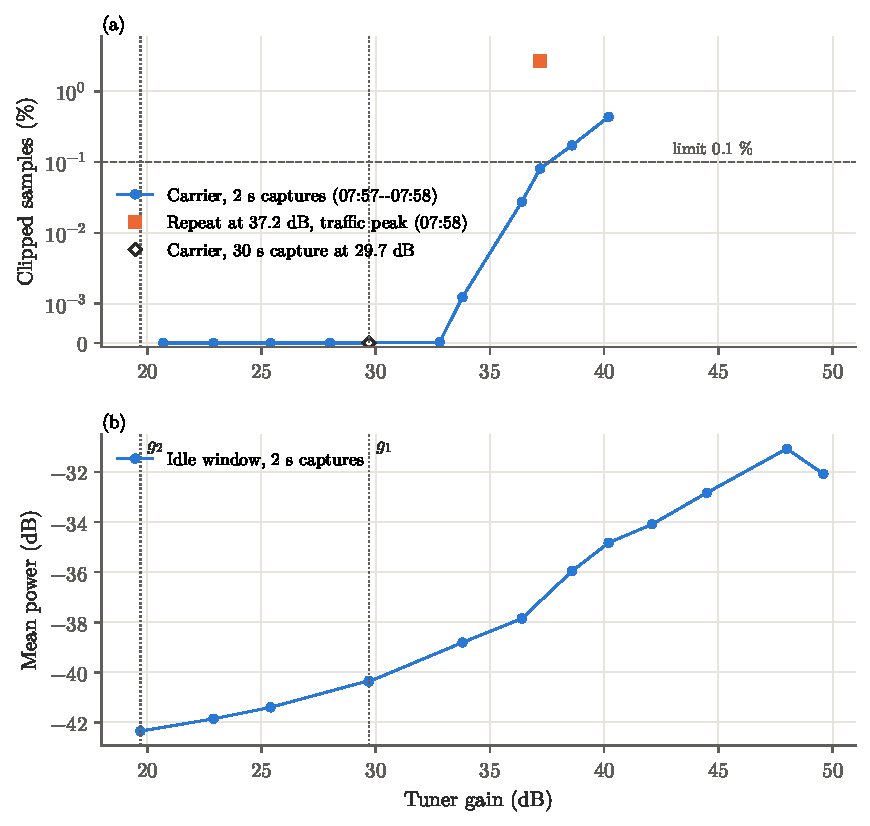
\includegraphics[width=\textwidth]{figA-gains}
  \caption[Gain trials]{Gain trials at P1, 5 November 2026. (a) Clipped samples in captures centred on the carrier, against the tuner gain, on a scale that is linear near zero and logarithmic above \pct{0.001}; the dashed line is the \pct{0.1} limit. (b) Mean power of captures of the idle window against the gain. Dotted lines: the chosen gains $g_1$ and $g_2$. Data of \cref{tab:app-gain-carrier,tab:app-gain-idle}.}
  \label{fig:app-gains}
\end{figure}

\emph{Choice of $g_1$.} Applied to the first series of carrier captures alone, the clipping limit would have given $g_1 = \qty{37.2}{\decibel}$, where \pct{0.081} of the samples clipped. A repeat at that gain about \qty{40}{\second} later, however, clipped \pct{2.70} of the samples: the carrier's mean power was \qty{6.7}{\decibel} higher (\qty{-3.93}{} against \qty{-10.58}{\decibel}), most probably because the power of a downlink carrier rises and falls with its traffic, whereas only its reference signals are always transmitted (\cref{sec:lte-sync}). A gain that respects the limit only when traffic is quiet would make clipped captures, which would have to be retaken, frequent at busy times. Retaking them until traffic is quiet would bias the data towards low traffic, so $g_1$ was instead chosen with a margin for such peaks: $g_1 = \qty{29.7}{\decibel}$, \qty{7.5}{\decibel} below \qty{37.2}{\decibel}. A traffic peak of the size observed brings the carrier at this gain to about the level it had at \qty{36.4}{\decibel} in quiet traffic, where \pct{0.028} of the samples clipped. A full-length capture at \qty{29.7}{\decibel}, during which the mean power in \qty{0.5}{\second} blocks varied over \qty{5.0}{\decibel}, had no clipped samples. The second gain is the tuner step \qty{10}{\decibel} lower, $g_2 = \qty{19.7}{\decibel}$, as agreed before the trials. Two alternatives were considered and set aside by the author: changing to the weaker carrier at \qty{783}{\mega\hertz}, which would have allowed a higher gain but would have reopened the choice of carrier and idle window, and a higher $g_1$ with clipped captures retaken, which would have biased the data as described above. The gains were confirmed by the author on 5 November 2026.

\emph{Consequence for the idle data.} Below about \qty{30}{\decibel} the idle level changed little with the gain: from \qty{-41.86}{\decibel} at \qty{22.9}{\decibel} to \qty{-40.38}{\decibel} at \qty{29.7}{\decibel}, \qty{1.5}{\decibel} for \qty{6.8}{\decibel} of gain. Above it, the level rose by roughly half a decibel per decibel of gain (\cref{fig:app-gains}). At these gains the idle level is therefore set mainly by the receiver's own noise rather than by what the antenna receives; at $g_1$ the idle samples had a standard deviation of only \num{0.86} converter steps. Lowering the gain from $g_1$ to $g_2$ lowered the idle level by \qty{2.0}{\decibel} (\qty{-40.34}{} to \qty{-42.35}{\decibel}), while the carrier fell by \qty{8.2}{\decibel} between \qty{29.7}{} and \qty{20.7}{\decibel}. Two expectations follow, and both are checked in every session: the captures with the antenna terminated (Class~A) and connected (Class~B) should differ little, and the gain-change test of H2 shifts the idle level by about \qty{2}{\decibel} rather than \qty{10}{\decibel} (\cref{sec:m-robustness}).

\section{Capture Sessions}
\label{app:sessions}

\TBC{One row per session: identifier, date and start time (UTC), position, gain settings $g_1$ and $g_2$, captures made, clipping flags and notes (\cref{sec:m-sessions}).}

\chapter{Code Listings}
\label{app:code}

% Author's request, 2 November 2026: the code and what it does; trimmed on
% 3 November 2026 to the modules that compute what the thesis reports (the rest
% is on GitHub); evaluate.py dropped on the author's request the same day, as
% Section 3.11 specifies the evaluation. The listings are read from the source files at compile time
% (\lstinputlisting), so they always match the code. Keep Table B.1 in step
% with code/occupancy/ and the test counts of Table B.2 with code/tests/.

% Keep the table of contents short: chapter and sections only in this appendix.
\addtocontents{toc}{\protect\setcounter{tocdepth}{1}}

The method of Chapter~3 is implemented in the Python package \texttt{occupancy}, in the folder \texttt{code/occupancy/} of the project, with its tests in \texttt{code/tests/} and the notebook and script for training on Google Colab in \texttt{code/colab/}. The complete code is available at \url{https://github.com/jimroxodezi/masters-thesis} (folder \texttt{code/}).% The author makes the repository public at submission (3 November 2026).


This appendix lists only the modules that compute what the thesis reports: the frames and the session-level folds, the spectrograms, the controlled-SNR test set, the detectors and their scores, the thresholds and the timing. The evaluation (pooling over the folds, metrics, session bootstrap and the tests of H1 and H2) is specified in full in \cref{sec:m-eval}, and its code is on GitHub. The other modules handle the capture, the file formats and records, the training runs, the Colab workflow, the demonstration, the command line and testing; \cref{tab:app-modules} describes every module in one line, and those not listed here can be read on GitHub. The listings are read from the source files when the thesis is compiled, so they match the code that produced the results. The version of the code is identified by the Git commit and a checksum of the source files, both recorded in every result file (the checksum alone for the models trained on Colab, where Git is not available): \TBC{commit and checksum of the final run}. Lines too long for the page are wrapped and marked with~$\hookrightarrow$.

The commands are run from the \texttt{code/} folder, for example \texttt{uv run python -m occupancy session} for a guided capture session (\texttt{--help} lists them all). The tests are run with \texttt{uv run python -m unittest discover -s tests}.

\begin{table}[tbp]
  \centering
  \small
  \caption[Modules of the code]{Modules of the code, by stage of the method. Only the modules with a section number are listed in this appendix; the others are on GitHub.}
  \label{tab:app-modules}
  \begin{tabularx}{\textwidth}{@{} >{\raggedright\arraybackslash}p{3.3cm} >{\raggedright\arraybackslash}X >{\raggedright\arraybackslash}p{1.9cm} @{}}
    \toprule
    Module & Purpose & Listing \\
    \midrule
    \texttt{config} & Every setting of the experiment & GitHub \\
    \texttt{provenance} & Code version, library versions, host and power state of every result & GitHub \\
    \texttt{iqio} & Raw capture files and their metadata records & GitHub \\
    \texttt{capture} & One capture, enforcing the capture rules (\cref{sec:m-capture}) & GitHub \\
    \texttt{session} & Guided capture session of eight captures (\cref{sec:m-sessions}) & GitHub \\
    \texttt{survey} & Band survey with \texttt{rtl\_power} (\cref{sec:m-survey}) & GitHub \\
    \texttt{quicklook} & Quick-look figures and the labelling check (\cref{sec:m-labels}) & GitHub \\
    \midrule
    \texttt{dataset} & Frames, DC removal and session-level folds (\cref{sec:m-splits}) & \Cref{app:code-data} \\
    \texttt{preprocess} & Spectrograms and their standardization (\cref{sec:m-preproc}) & \Cref{app:code-data} \\
    \texttt{injection} & Controlled-SNR test set (\cref{sec:m-injection}) & \Cref{app:code-data} \\
    \midrule
    \texttt{models} & The three networks, the PER score and the scoring copy (\cref{sec:m-detectors,sec:m-optim}) & \Cref{app:code-detectors} \\
    \texttt{pss} & PSS correlator (\cref{sec:m-pss}) & \Cref{app:code-detectors} \\
    \texttt{detectors} & Scores of every detector & \Cref{app:code-detectors} \\
    \texttt{train} & Training of the networks and fitting of PCA, with checkpoints and resume (\cref{sec:m-training}) & GitHub \\
    \midrule
    \texttt{scoring} & Frames that each fold scores, and score files & GitHub \\
    \texttt{calibrate} & Thresholds at fixed false-alarm rates (\cref{sec:m-thresholds}) & \Cref{app:code-eval} \\
    \texttt{evaluate} & Metrics, session bootstrap and the tests of H1 and H2 (\cref{sec:m-eval}) & GitHub \\
    \midrule
    \texttt{latency} & Latency, throughput, real-time factor and the effect of the optimization (\cref{sec:m-compute}) & \Cref{app:code-cost} \\
    \texttt{realtime} & Real-time demonstration (\cref{sec:m-demo}) & GitHub \\
    \midrule
    \texttt{device}, \texttt{pack}, \texttt{unpack}, \texttt{budget} & Training device, training pack for Colab, import of the trained models, compute budget & GitHub \\
    \texttt{colab/} & Script and notebook for training on the Colab GPU & GitHub \\
    \texttt{cli}, \texttt{\_\_main\_\_}, \texttt{\_\_init\_\_} & Command line and package entry point & GitHub \\
    \texttt{synthetic} & Synthetic test data, never used for a result & GitHub \\
    \texttt{tests/} & Tests of the code (\cref{tab:app-tests}) & GitHub \\
    \bottomrule
  \end{tabularx}
\end{table}

\begin{singlespace}

\section{Data Preparation}
\label{app:code-data}

\subsection*{\texttt{occupancy/dataset.py}}
Builds the index of all captures from their metadata records, refusing synthetic captures unless they are explicitly allowed and never mixing them with real ones. It cuts each capture into non-overlapping frames of \num{16384} samples with the frame mean removed, and forms the session-level folds of \cref{sec:m-splits}.
\lstinputlisting{code/occupancy/dataset.py}

\subsection*{\texttt{occupancy/preprocess.py}}
Computes the spectrogram of each frame (\cref{sec:m-preproc}) and the global standardization fitted on a fold's training frames only. The spectrograms are stored on disk as half-precision arrays, one file per capture.
\lstinputlisting{code/occupancy/preprocess.py}

\subsection*{\texttt{occupancy/injection.py}}
Builds the controlled-SNR test set of \cref{sec:m-injection} for each test session, gain and source class: the power estimates, the scale factor $\alpha$, the effective SNR of each mixture and the admissibility rule for the active frames. The random choice of frames is seeded, so the set can be rebuilt exactly.
\lstinputlisting{code/occupancy/injection.py}

\section{Detectors}
\label{app:code-detectors}

\subsection*{\texttt{occupancy/models.py}}
The three neural networks of \cref{sec:m-convae,sec:m-fcae,sec:m-vae}: the convolutional autoencoder, the fully connected autoencoder and the convolutional VAE, with the percentile score of \textcite{tian2022} and the list of models and ablations to train. It also prepares the copy of a trained network with which every score is computed (\cref{sec:m-optim}): each batch-normalization layer is folded into the convolution before it, and the convolutional networks use the channels-last memory order. The original percentile computation is kept as the reference that the tests and the timing compare with.
\lstinputlisting{code/occupancy/models.py}

\subsection*{\texttt{occupancy/pss.py}}
The \syncsignal{} correlator (\cref{sec:m-pss}): the three PSS Zadoff--Chu sequences, their mapping to subcarriers, the 128-sample time-domain templates and the normalized correlation of \cref{eq:m-pss}, computed with FFTs over every lag at which the template lies inside the frame.
\lstinputlisting{code/occupancy/pss.py}

\subsection*{\texttt{occupancy/detectors.py}}
Computes the score of every detector on the same DC-removed frames: the reconstruction errors of the networks and of PCA, the percentile score, the average power for the fixed energy detector, the running noise estimate of the adaptive energy detector, and the PSS correlation.
\lstinputlisting{code/occupancy/detectors.py}

\section{Calibration}
\label{app:code-eval}

\subsection*{\texttt{occupancy/calibrate.py}}
Sets the thresholds of \cref{sec:m-thresholds} for every detector, fold and seed, as the empirical quantile of the idle validation scores, including the constant $\kappa$ of the adaptive energy detector and the theoretical chi-square threshold reported for comparison.
\lstinputlisting{code/occupancy/calibrate.py}

\section{Computational Cost}
\label{app:code-cost}

\subsection*{\texttt{occupancy/latency.py}}
Measures the computational cost on the laptop (\cref{sec:m-timing}). After a settling period of \qty{5}{\second} and a warm-up, it times each detector frame by frame, separately for preprocessing, for scoring and end to end, and measures the throughput with batches of 64 frames and the real-time factor. It also times each neural network as trained and in its scoring form, alternating frame by frame, to measure the effect of the optimization of \cref{sec:m-optim}. It refuses to time unless the laptop is on mains power with the Performance power profile.
\lstinputlisting{code/occupancy/latency.py}

\section{Tests}
\label{app:code-tests}

The tests check the parts of the method that can be checked without real data (\cref{tab:app-tests}). They run on the laptop in under a minute. The end-to-end test uses a tiny synthetic data set and checks only that the stages connect correctly; its numbers mean nothing.

% Keep the counts in step with code/tests/ (grep -c "def test_" code/tests/test_*.py).
\begin{table}[tbp]
  \centering
  \small
  \caption[Tests of the code]{Tests of the code in \texttt{code/tests/}. All 94 tests pass.}
  \label{tab:app-tests}
  \begin{tabularx}{\textwidth}{@{} >{\raggedright\arraybackslash}p{4.1cm} >{\raggedright\arraybackslash}X r @{}}
    \toprule
    File & What it checks & Tests \\
    \midrule
    \texttt{test\_capture\_io} & Frequency parsing; manual gain, gain steps and tuning range; the offset-window rule; the capture file format and metadata; stopping a capture safely & 11 \\
    \texttt{test\_session} & Capture order; omission of C\textsubscript{offset} for narrow carriers; retakes; resuming an interrupted session & 4 \\
    \texttt{test\_survey} & Reading \texttt{rtl\_power} output; the command used; suggested carriers and Class~B windows & 4 \\
    \texttt{test\_split} & Folds for twelve and other numbers of sessions; session order & 4 \\
    \texttt{test\_preprocess} & Spectrogram shape, bin spacing and orientation; the Hann window and decibel scale; DC removal; normalization from training data only & 5 \\
    \texttt{test\_injection} & SNR grid; scale factor; effective SNR within \qty{0.5}{\decibel} of the target; admissibility; reproducible draws & 5 \\
    \texttt{test\_pss} & PSS sequences and their subcarrier mapping; templates; detection of a PSS but not of noise & 7 \\
    \texttt{test\_models} & Shapes of the three networks; the percentile score; one training epoch & 7 \\
    \texttt{test\_ed\_adaptive} & The adaptive energy detector, including that occupied frames do not update the noise estimate and that $\kappa$ is calibrated on an idle stream & 5 \\
    \texttt{test\_calibrate} & Thresholds give at most the requested false-alarm rate; decisions are strict; the chi-square threshold & 4 \\
    \texttt{test\_bootstrap} & Session-bootstrap intervals are reproducible with a fixed seed & 3 \\
    \texttt{test\_synthetic\_guard} & Synthetic data are marked, refused without the flag and never mixed with real data & 6 \\
    \texttt{test\_pipeline} & End-to-end run on a tiny synthetic data set (plumbing only) & 6 \\
    \texttt{test\_resume} & An interrupted and resumed training run ends in the same state as an uninterrupted one; a checkpoint written with other settings is not resumed; a finished run is retrained only on request; the fallback to the CPU; the record of the runtime environment & 5 \\
    \texttt{test\_cost\_and\_demo} & The scoring copy of each network gives the same reconstructions; the percentile score equals the original computation; both forms of each network are timed; the power-condition check; the demonstration's queue, lost-sample estimate and live-view limits & 8 \\
    \texttt{test\_colab} & The pack holds only Class~B spectrograms at $g_1$; corrupted packs and unsafe zip files are refused; training from the pack gives the same models as training from the local data; training through the Colab script without the receiver library; unpacking; the epoch-timing output; a valid notebook & 10 \\
    \texttt{helpers} & Shared test helpers (tiny configurations and data sets) & --- \\
    \bottomrule
  \end{tabularx}
\end{table}

\end{singlespace}

\chapter{Software Installation}
\label{app:install}

% Added 4 November 2026 at the author's request ("add the installation steps
% of important software"). Every command was either taken from the cited guide
% or run on the host laptop; keep it in step with code/README.md.

The software runs on the host laptop under Ubuntu 26.04 LTS (\cref{tab:m-hw-sw}). Three components are installed on it: the receiver driver, the Python environment of the study's code, and the cell-search tool. The commands below are typed in a terminal. Training on Google Colab needs no installation on the laptop: the notebook copies the code to the Colab runtime and installs any missing Python packages there (\cref{sec:m-training}).

\begin{singlespace}

\section{Receiver Driver}
\label{app:install-driver}

The RTL-SDR Blog V4 needs a version of the RTL-SDR library that supports its R828D tuner. The host laptop uses the manufacturer's fork of the library, \texttt{rtl-sdr-blog} \parencite{rtlsdrblog2026}, at commit aed0ea1 (22 March 2026), built from source with the fork's instructions for Linux:
\begin{lstlisting}[language=bash]
sudo apt update
sudo apt install libusb-1.0-0-dev git cmake pkg-config
git clone https://github.com/rtlsdrblog/rtl-sdr-blog
cd rtl-sdr-blog/
mkdir build
cd build
cmake ../ -DINSTALL_UDEV_RULES=ON
make
sudo make install
sudo cp ../rtl-sdr.rules /etc/udev/rules.d/
sudo ldconfig
\end{lstlisting}
The build installs the library in \texttt{/usr/local/lib}, together with \texttt{rtl\_test} and the survey tool \texttt{rtl\_power}. The television drivers of the Linux kernel, which would otherwise claim the receiver, are disabled by a file in \texttt{/etc/modprobe.d/} that blacklists the modules \texttt{dvb\_usb\_rtl28xxu}, \texttt{rtl2832} and \texttt{rtl2830}.

The capture program records the library it loaded with every capture, and \texttt{rtl\_test -t} identifies the receiver:
\begin{lstlisting}[language=bash]
Found 1 device(s):
  0:  RTLSDRBlog, Blog V4, SN: 00000001
Found Rafael Micro R828D tuner
RTL-SDR Blog V4 Detected
\end{lstlisting}
It also lists the 29 gain steps of the tuner, from \qty{0.0}{\decibel} to \qty{49.6}{\decibel}; the gains $g_1$ and $g_2$ are chosen from these steps.

\section{Python Environment}
\label{app:install-python}

The study's code (\cref{app:code}) runs in a Python environment managed by the package manager uv. The project's lock file, \texttt{code/uv.lock}, fixes the version of every package (\cref{tab:m-hw-sw}), so the environment is created with one command in the \texttt{code/} folder. Two further commands check that the code can see the receiver and that its tests pass:
\begin{lstlisting}[language=bash]
cd code
uv sync
uv run python -m occupancy capture --info
uv run python -m unittest discover -s tests
\end{lstlisting}
The receiver check reports the product name (Blog V4), the tuner (R828D) and its gain steps.

\section{Cell-Search Tool}
\label{app:install-cellsearch}

LTE-Cell-Scanner \parencite{peroulas2024} is built from source. Its last change (commit e7f71cb) dates from January 2024, before the versions of CMake (4.2) and Boost (1.90) in Ubuntu 26.04, so two adjustments are needed. Boost's \texttt{system} component is now part of the Boost headers and is no longer a separate library, so it is removed from the project's list of Boost components; and CMake is told to accept the project's old minimum version. The optional OpenCL acceleration is not built, so the program runs on the CPU:
\begin{lstlisting}[language=bash]
sudo apt install libitpp-dev libblas-dev liblapack-dev libfftw3-dev libboost-thread-dev libncurses-dev
mkdir -p ~/tools && cd ~/tools
git clone https://github.com/JiaoXianjun/LTE-Cell-Scanner.git
cd LTE-Cell-Scanner
sed -i 's/COMPONENTS thread system REQUIRED/COMPONENTS thread REQUIRED/' CMakeLists.txt
mkdir build && cd build
cmake .. -DUSE_OPENCL=0 -DCMAKE_POLICY_VERSION_MINIMUM=3.5
make -j4
\end{lstlisting}
Two checks confirm the build: the program must use the RTL-SDR library of \cref{app:install-driver}, and it must print its options:
\begin{lstlisting}[language=bash]
ldd src/CellSearch | grep rtlsdr    # /usr/local/lib/librtlsdr.so.0
./src/CellSearch -h
\end{lstlisting}
A search around a plateau found in the survey, for example one centred near \qty{796}{\mega\hertz}, is then run with a fixed gain (in decibels) and two tries at each frequency:
\begin{lstlisting}[language=bash]
./src/CellSearch -s 795.5e6 -e 796.5e6 -g 40.2 -n 2
\end{lstlisting}
At each session, the search is repeated at the chosen carrier's frequency alone, and the samples it captured are kept with the session's records (\texttt{--recbin}). Only \texttt{CellSearch} is used; the scanner's tracking program, \texttt{LTE-Tracker}, is not (\cref{sec:m-ethics}).

\end{singlespace}


\end{document}
